%!TEX root = ../TTK4550-MHT.tex

\begin{appendices}
	\section{Track performance plots}
	%!TEX root = ../TTK4550-MHT.tex
\begin{figure}[H]
    \centering
    \textbf{Scenario 1 - Track performance}\par \medskip
    \begin{subfigure}{0.49\textwidth}
        \centering
        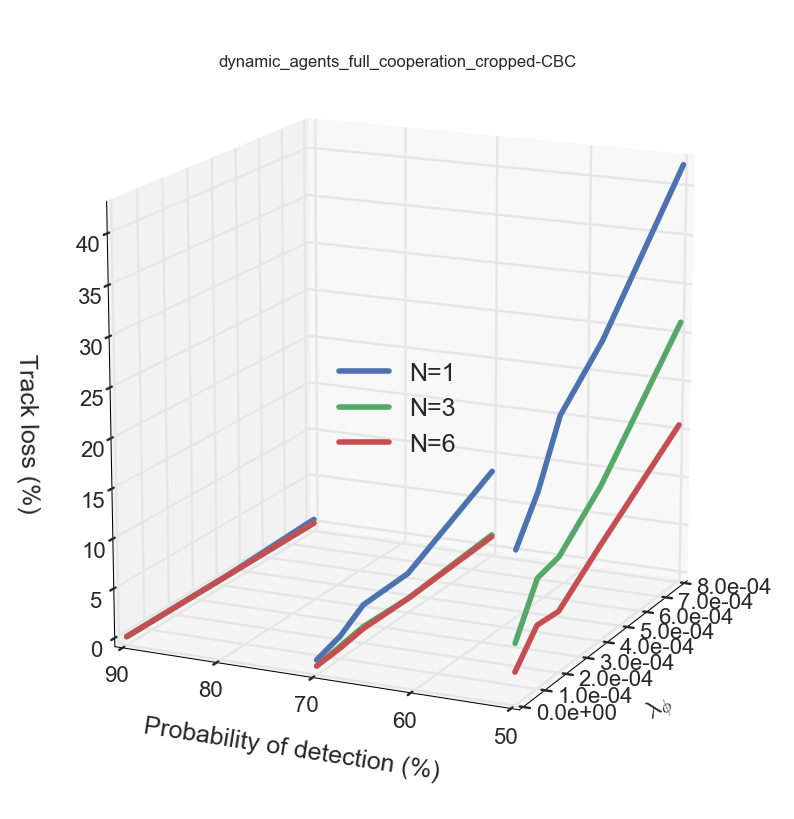
\includegraphics[width=\textwidth]{dynamic_agents_full_cooperation_cropped-CBC}
        \caption{CBC solver}
    \end{subfigure}
    \begin{subfigure}{0.49\textwidth}
        \centering
        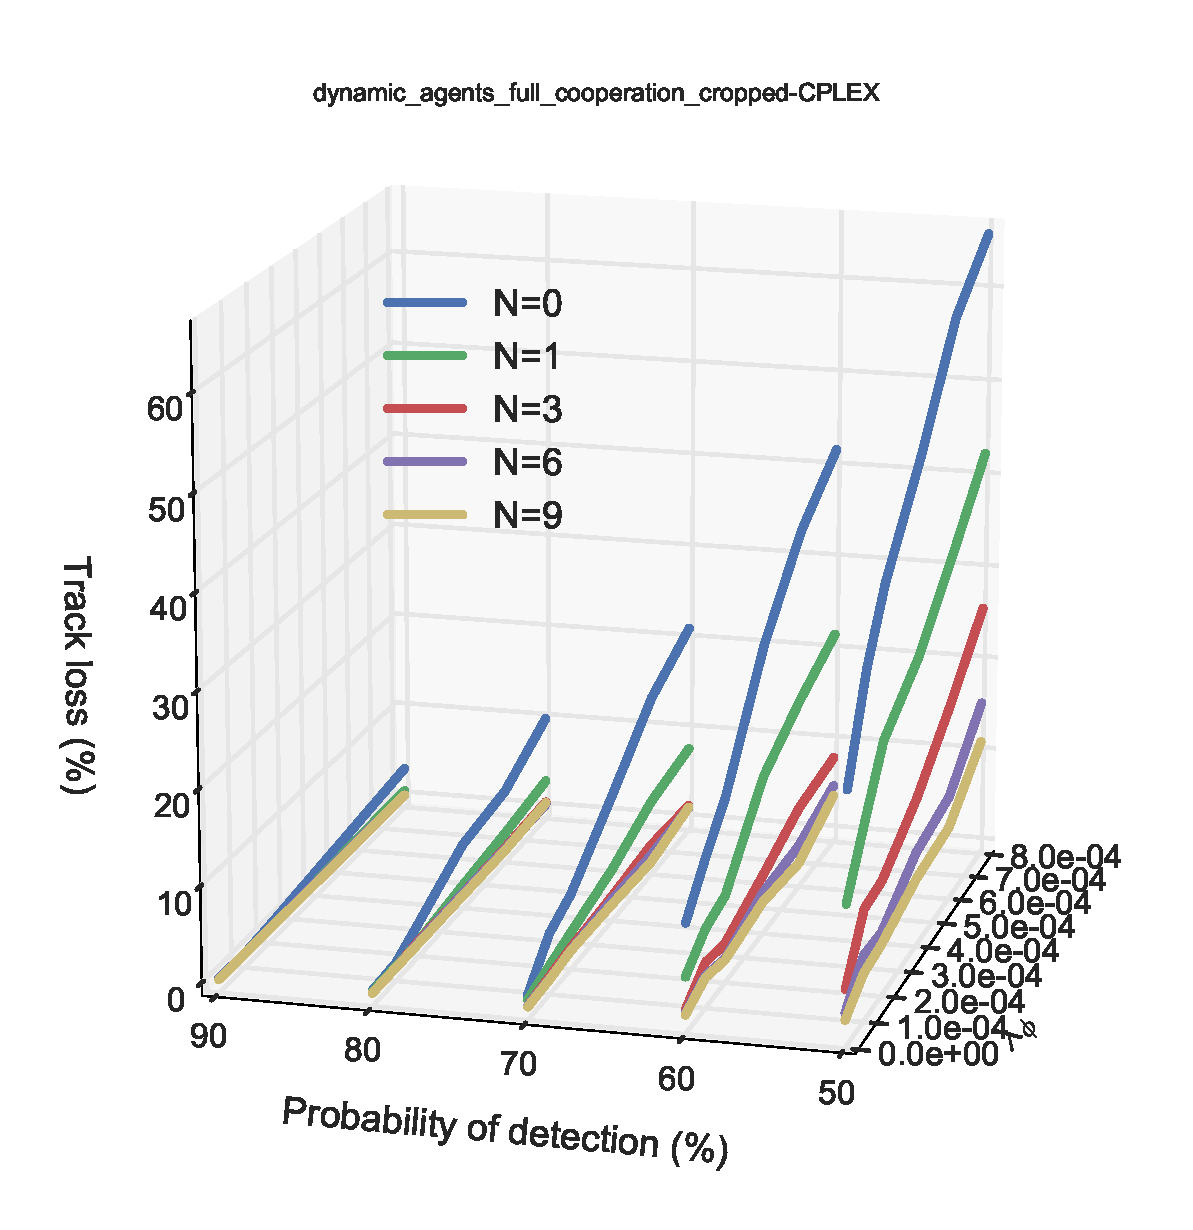
\includegraphics[width=\textwidth]{dynamic_agents_full_cooperation_cropped-CPLEX}
        \caption{CPLEX solver}
    \end{subfigure}
    \begin{subfigure}{0.49\textwidth}
        \centering
        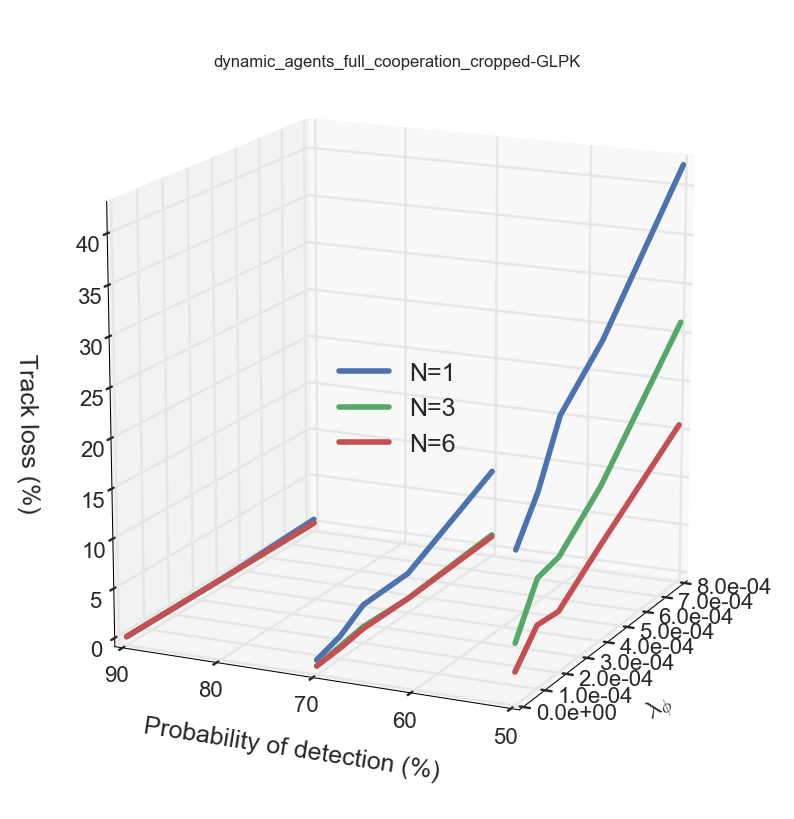
\includegraphics[width=\textwidth]{dynamic_agents_full_cooperation_cropped-GLPK}
        \caption{GLPK solver}
    \end{subfigure}
    \begin{subfigure}{0.49\textwidth}
        \centering
        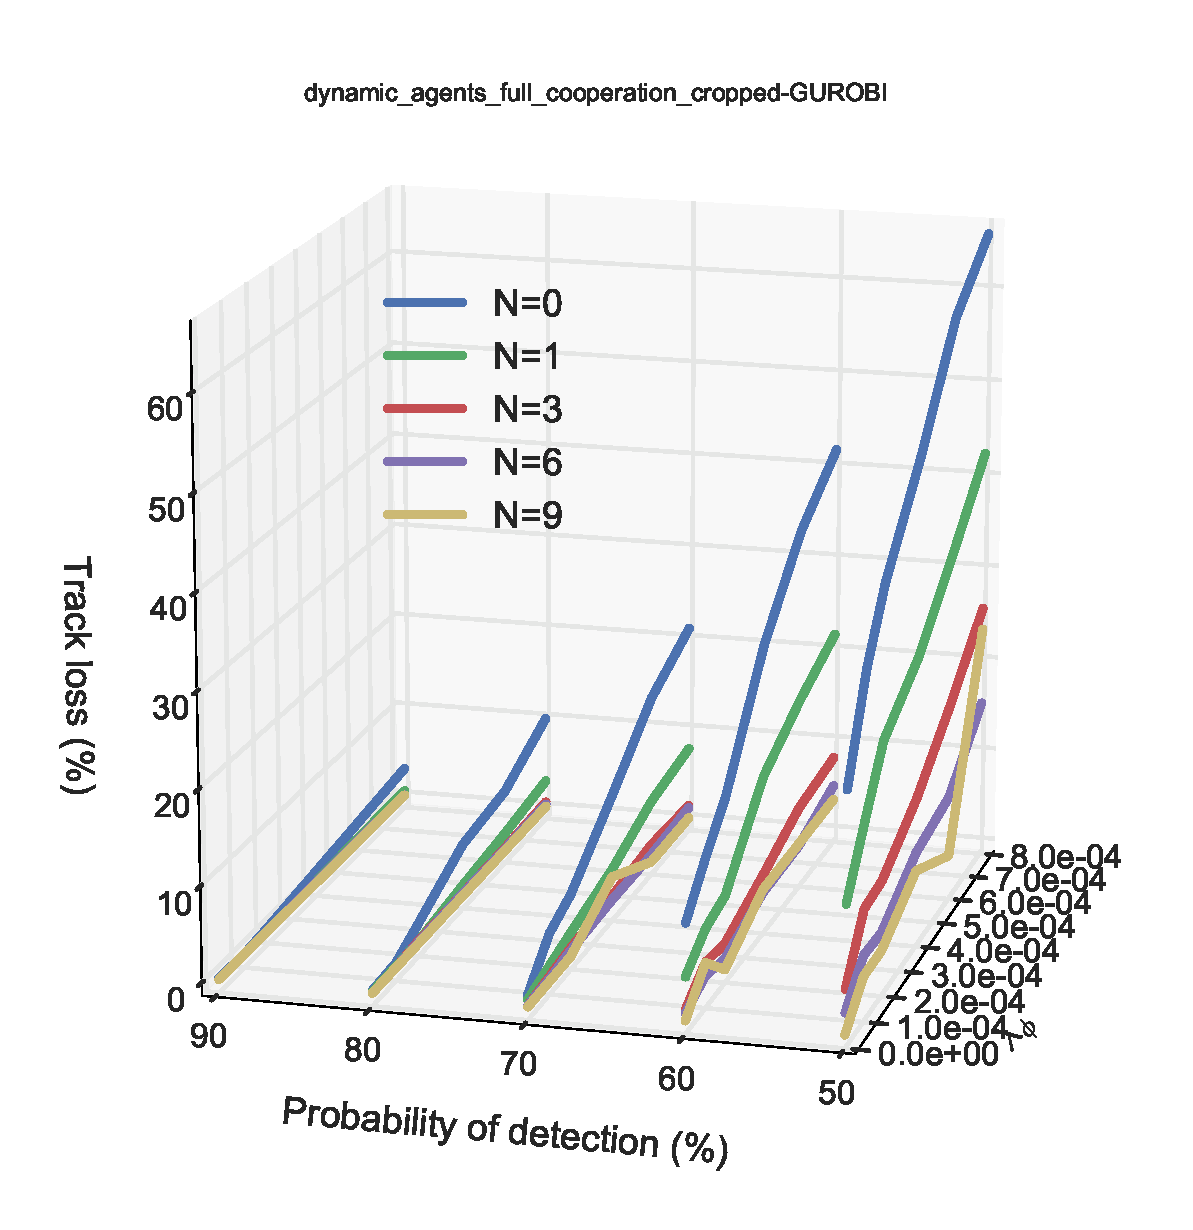
\includegraphics[width=\textwidth]{dynamic_agents_full_cooperation_cropped-GUROBI}
        \caption{GUROBI solver}
    \end{subfigure}
	\caption{Simulation results for all solvers in scenario 1}
    \label{fig:dynamic_agents_full_cooperation_cropped}
\end{figure}

\begin{figure}[H]
    \centering
    \textbf{Scenario 2 - Track performance}\par \medskip
    \begin{subfigure}{0.49\textwidth}
        \centering
        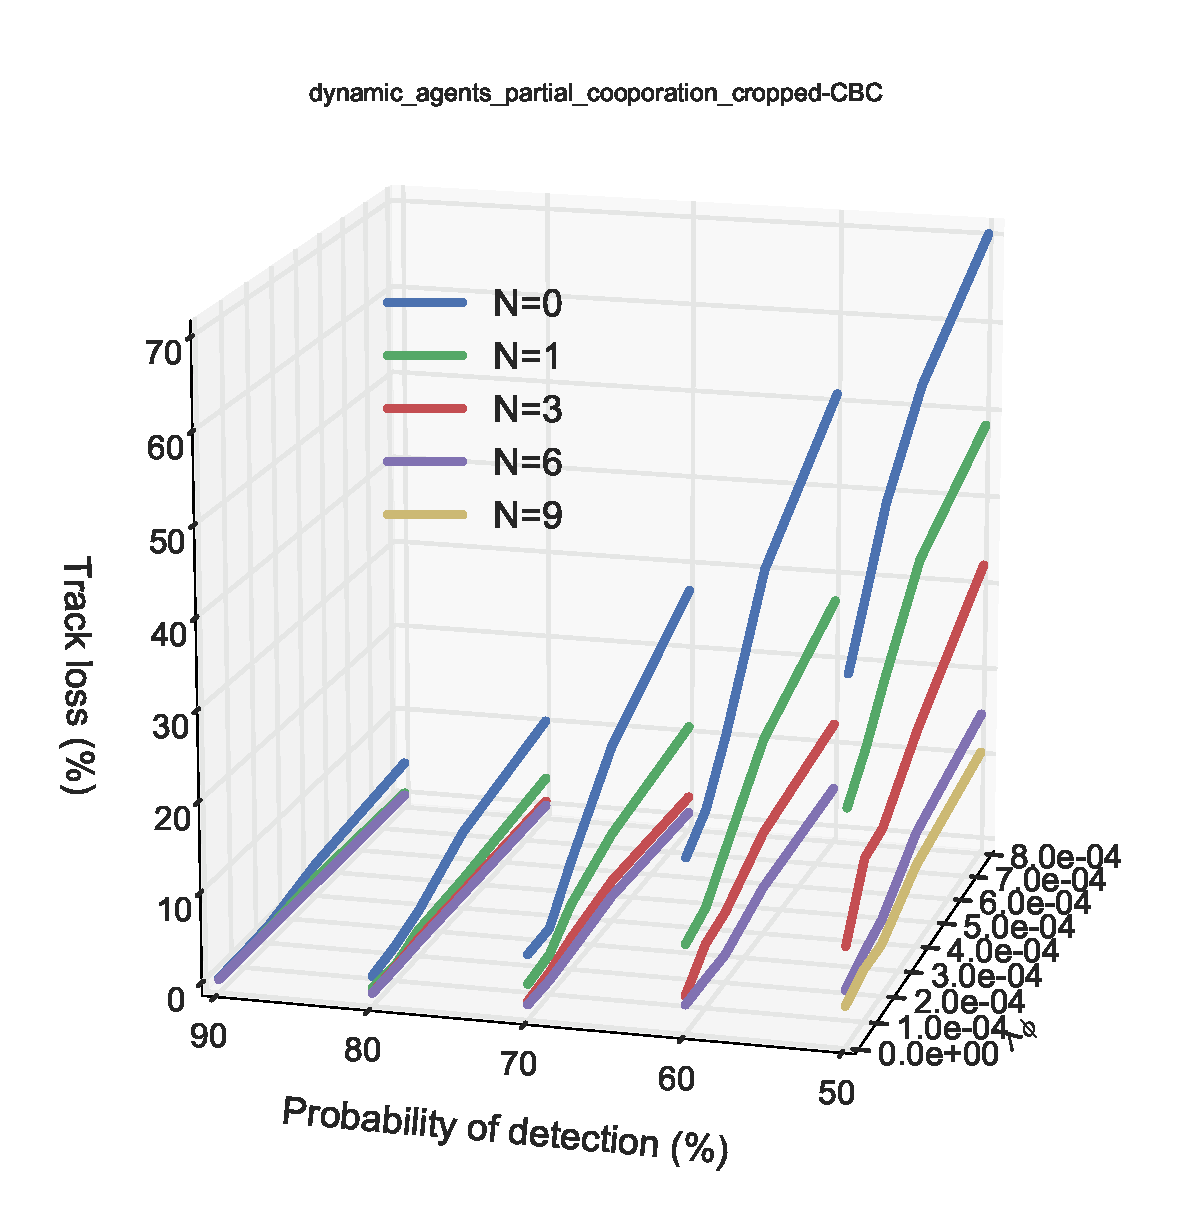
\includegraphics[width=\textwidth]{dynamic_agents_partial_cooporation_cropped-CBC}
        \caption{CBC solver}
    \end{subfigure}
    \begin{subfigure}{0.49\textwidth}
        \centering
        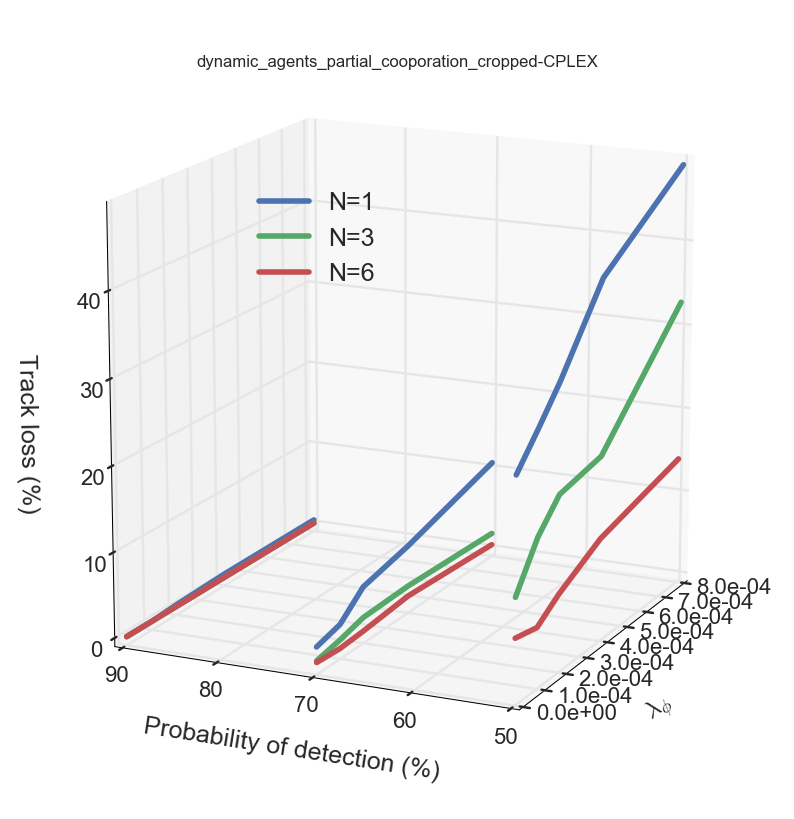
\includegraphics[width=\textwidth]{dynamic_agents_partial_cooporation_cropped-CPLEX}
        \caption{CPLEX solver}
    \end{subfigure}
    \begin{subfigure}{0.49\textwidth}
        \centering
        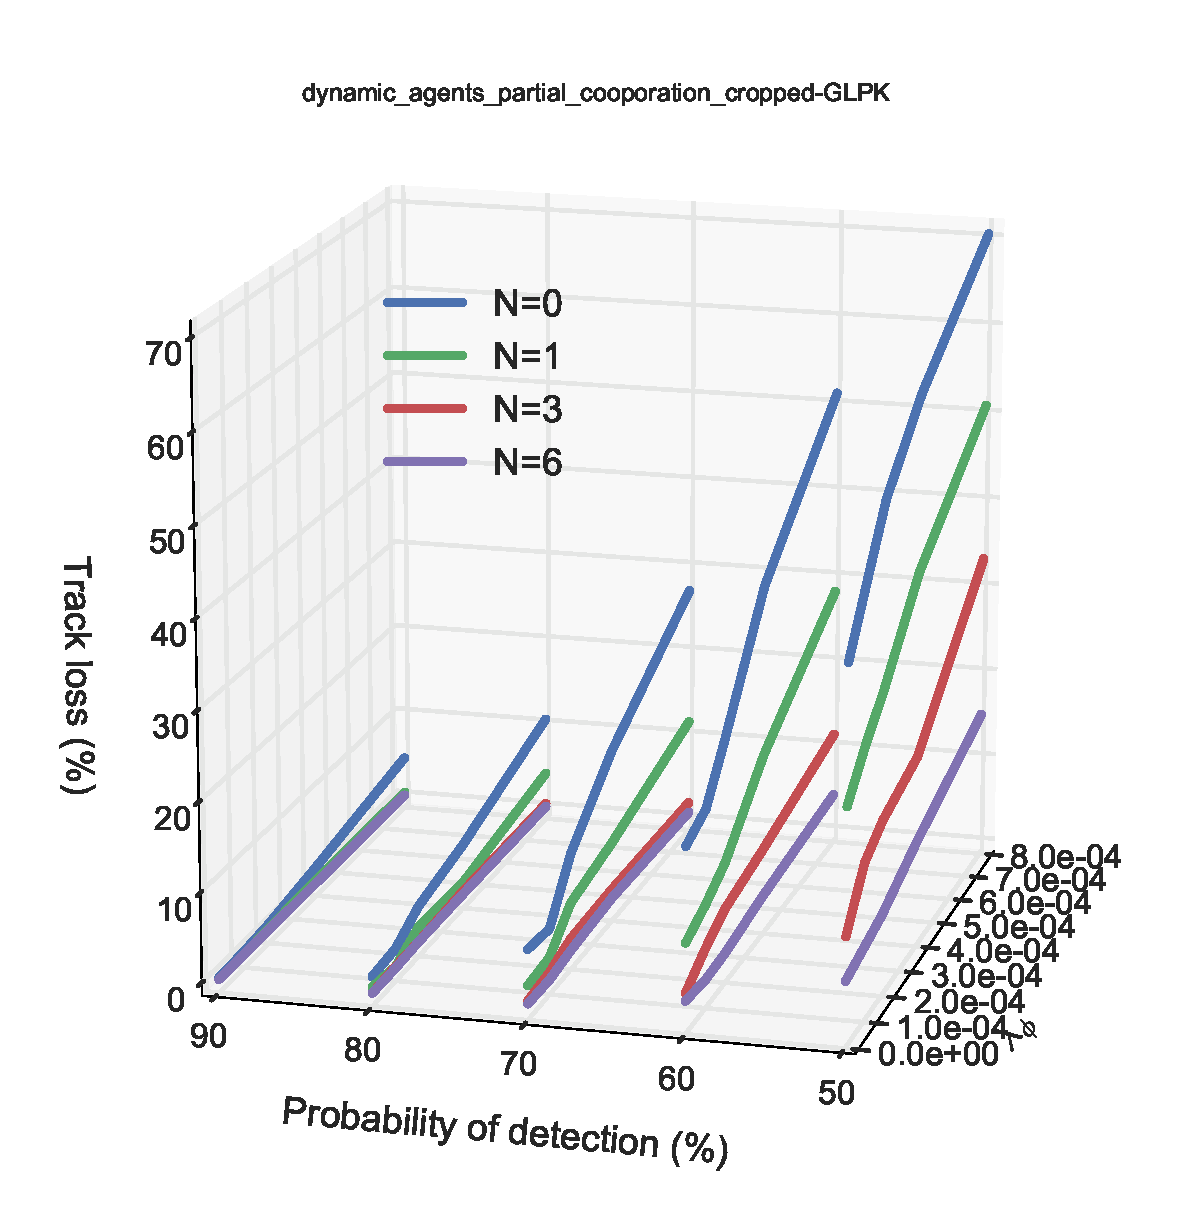
\includegraphics[width=\textwidth]{dynamic_agents_partial_cooporation_cropped-GLPK}
        \caption{GLPK solver}
    \end{subfigure}
    \begin{subfigure}{0.49\textwidth}
        \centering
        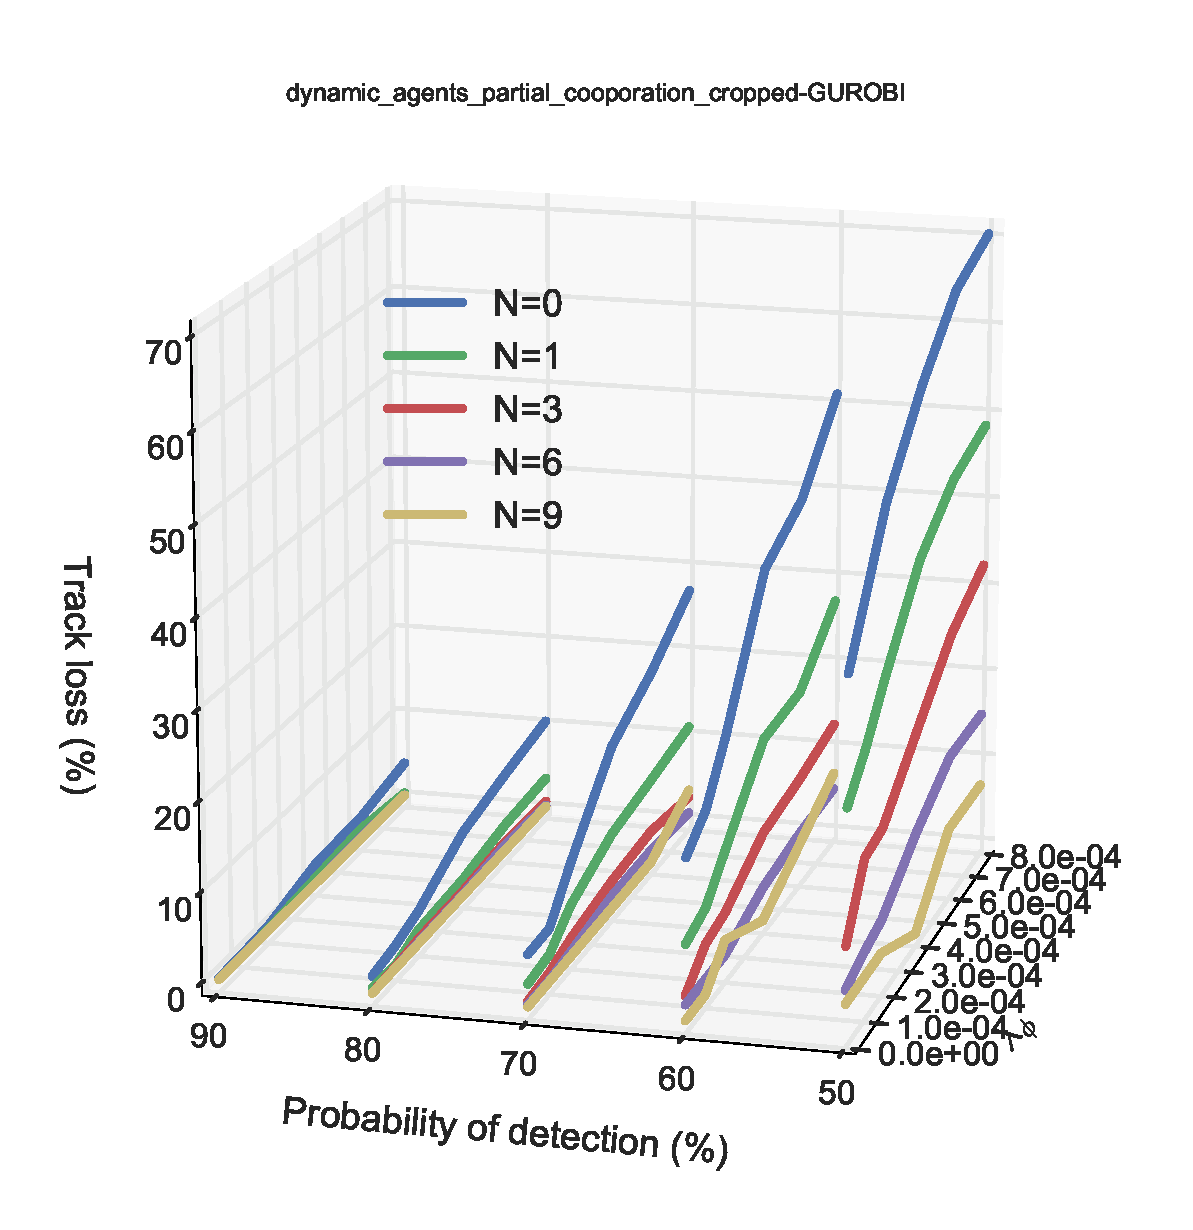
\includegraphics[width=\textwidth]{dynamic_agents_partial_cooporation_cropped-GUROBI}
        \caption{GUROBI solver}
    \end{subfigure}
    \caption{Simulation results for all solvers in scenario 2}
	\label{fig:dynamic_agents_partial_cooperation_cropped}
\end{figure}

\begin{figure}[H]
    \centering
    \textbf{Scenario3 - Track performance}\par \medskip
    \begin{subfigure}{0.49\textwidth}
        \centering
        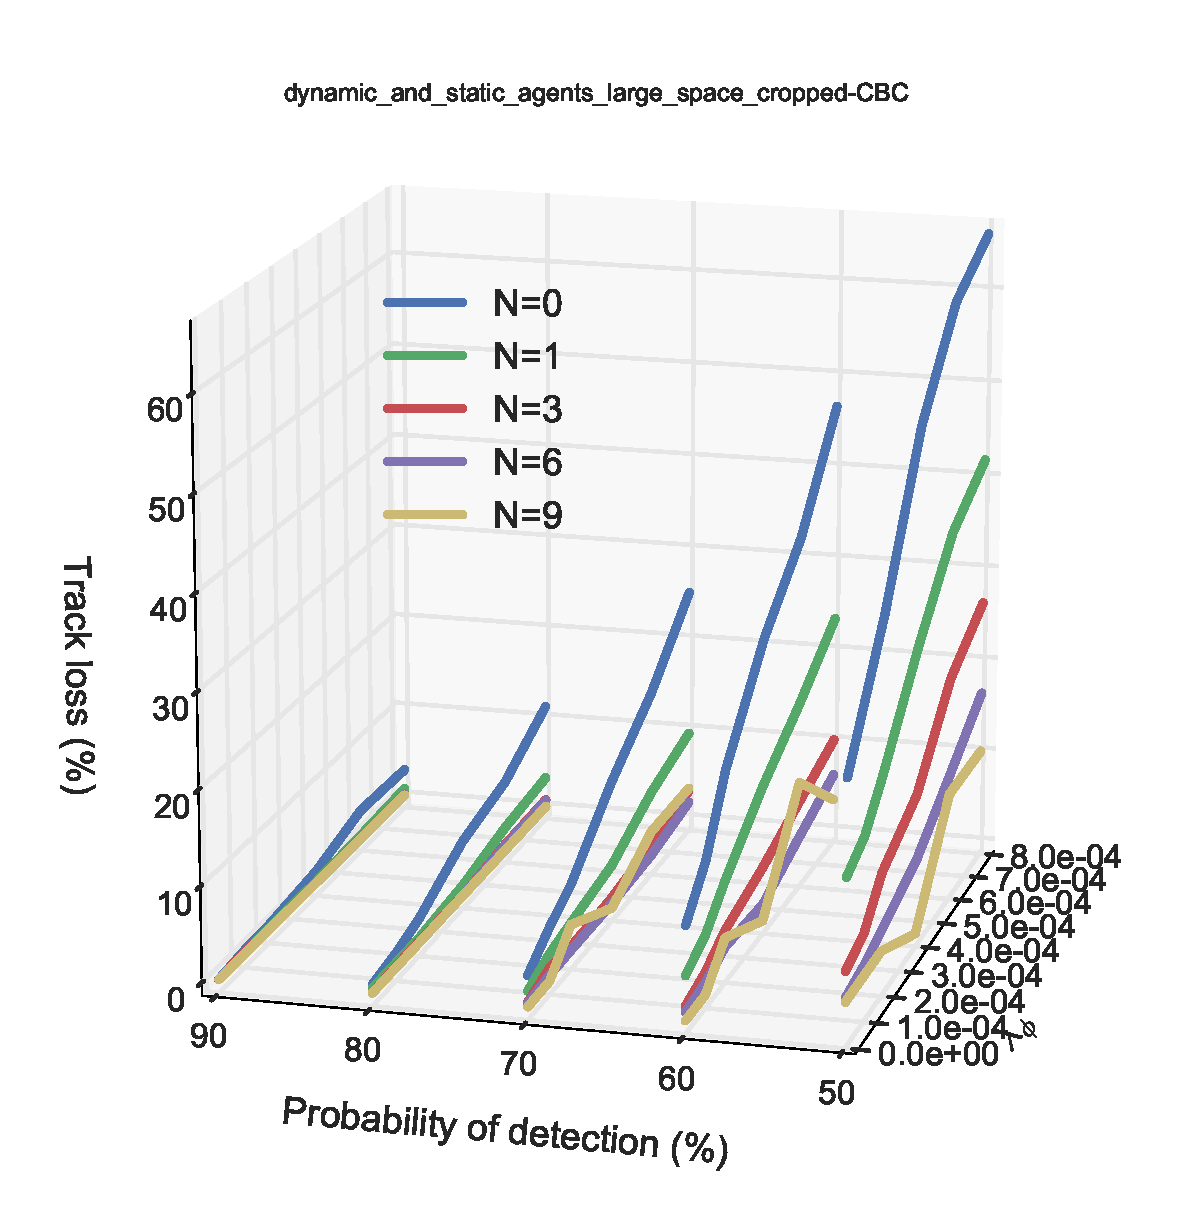
\includegraphics[width=\textwidth]{dynamic_and_static_agents_large_space_cropped-CBC}
        \caption{CBC solver}
    \end{subfigure}
    \begin{subfigure}{0.49\textwidth}
        \centering
        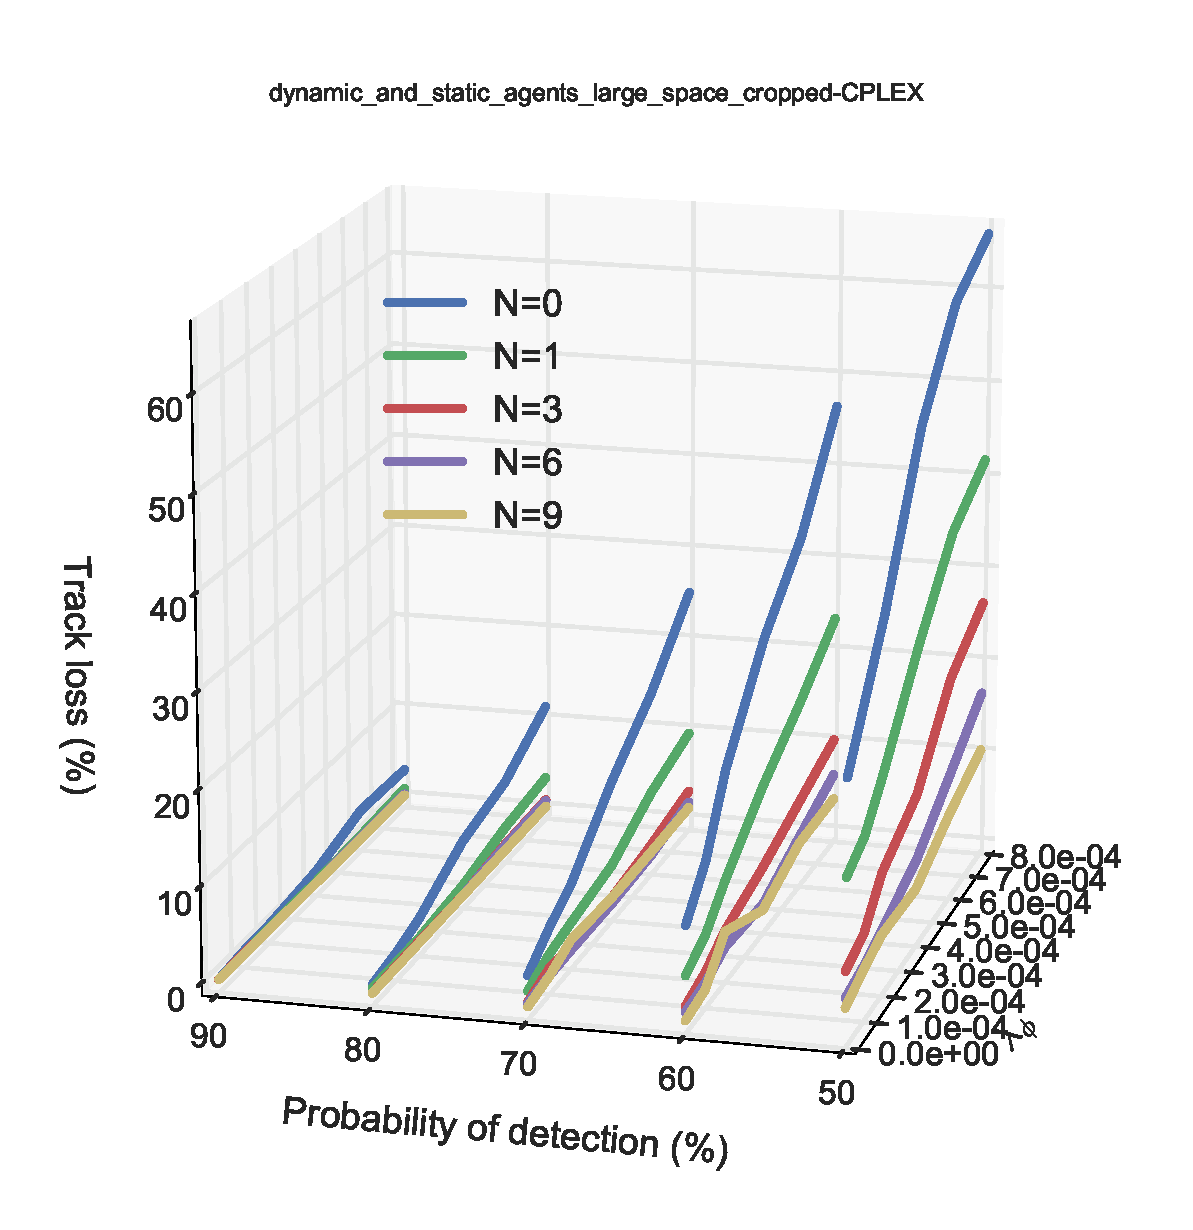
\includegraphics[width=\textwidth]{dynamic_and_static_agents_large_space_cropped-CPLEX}
        \caption{CPLEX solver}
    \end{subfigure}
    \begin{subfigure}{0.49\textwidth}
        \centering
        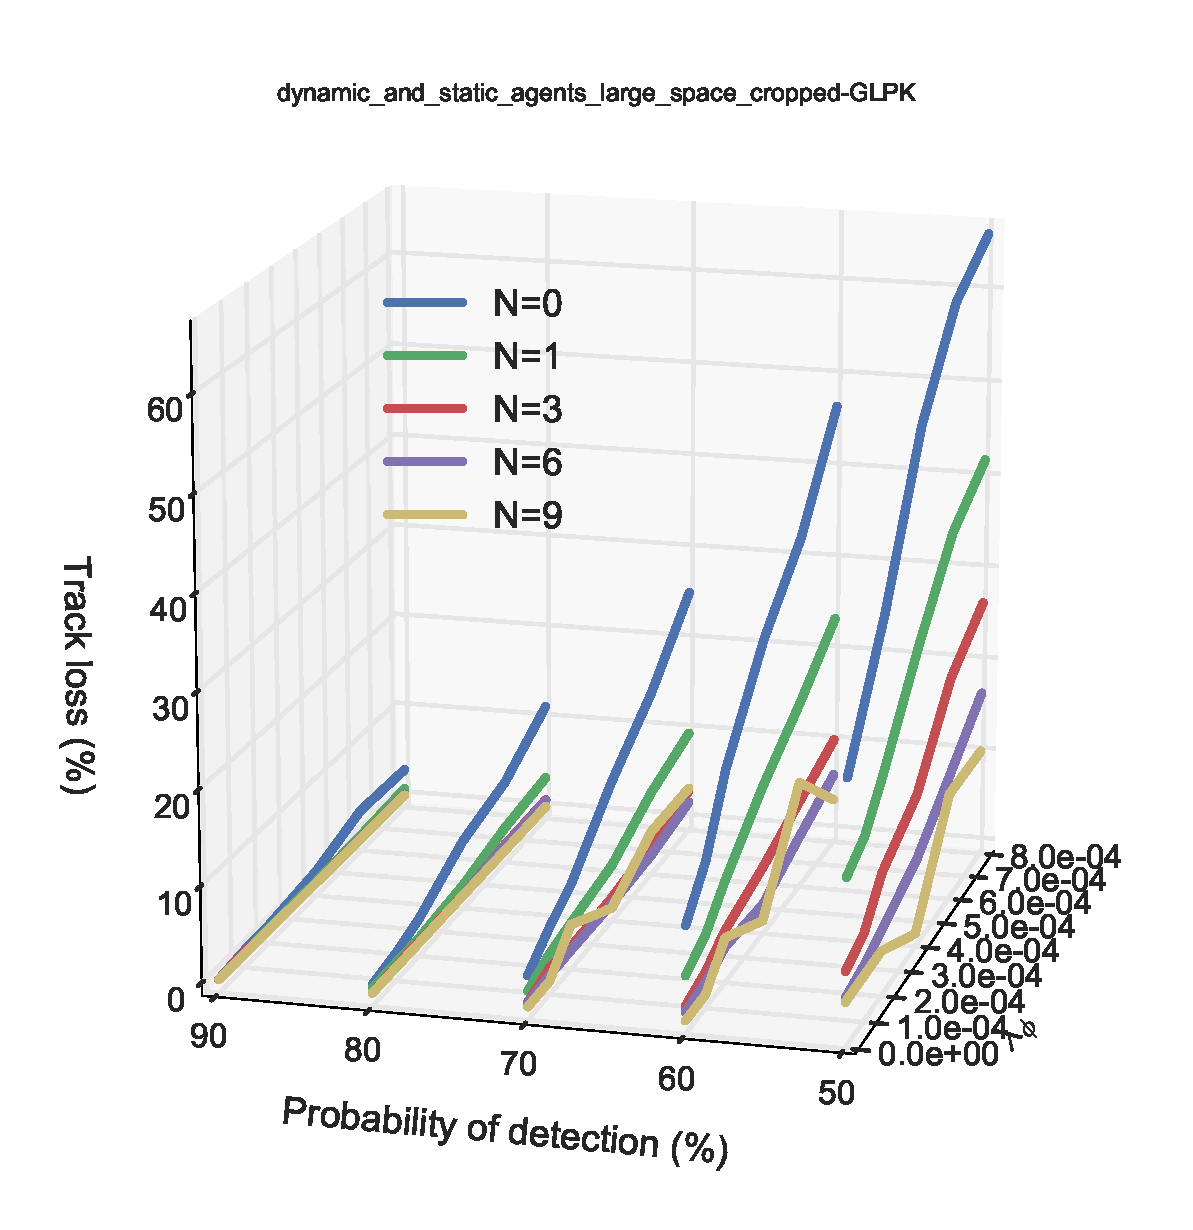
\includegraphics[width=\textwidth]{dynamic_and_static_agents_large_space_cropped-GLPK}
        \caption{GLPK solver}
    \end{subfigure}
    \begin{subfigure}{0.49\textwidth}
        \centering
        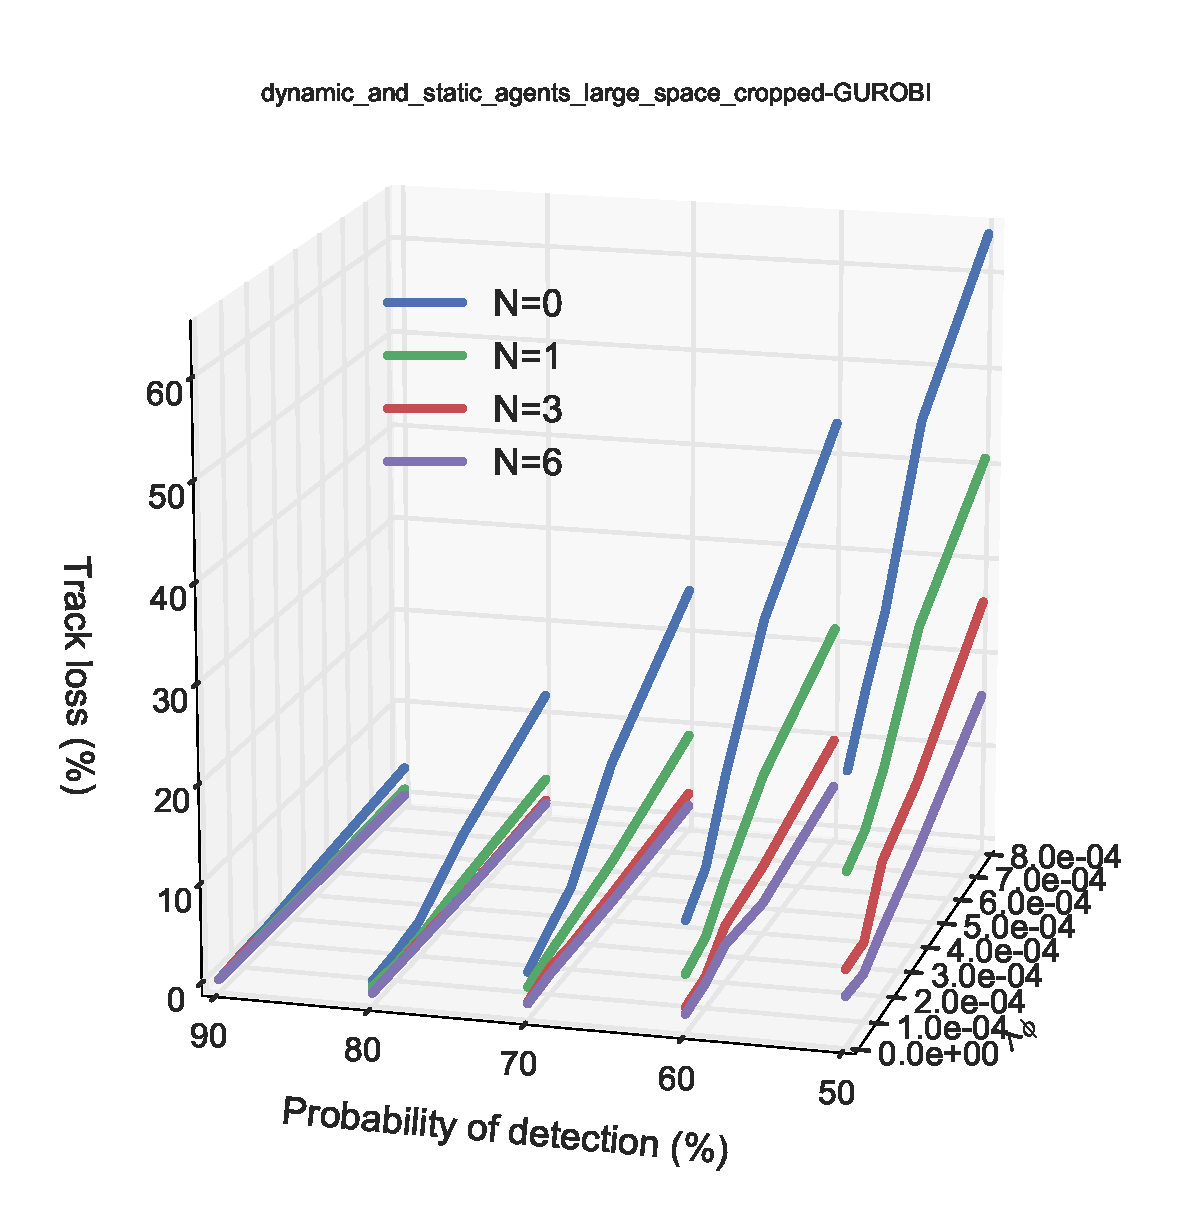
\includegraphics[width=\textwidth]{dynamic_and_static_agents_large_space_cropped-GUROBI}
        \caption{GUROBI solver}
    \end{subfigure}
    \caption{Simulation results for all solvers in scenario 3}
	\label{fig:dynamic_and_static_agents_large_space_cropped}
\end{figure}

\begin{figure}[H]
    \centering
    \textbf{Scenario 4 - Track performance}\par \medskip
    \begin{subfigure}{0.49\textwidth}
        \centering
        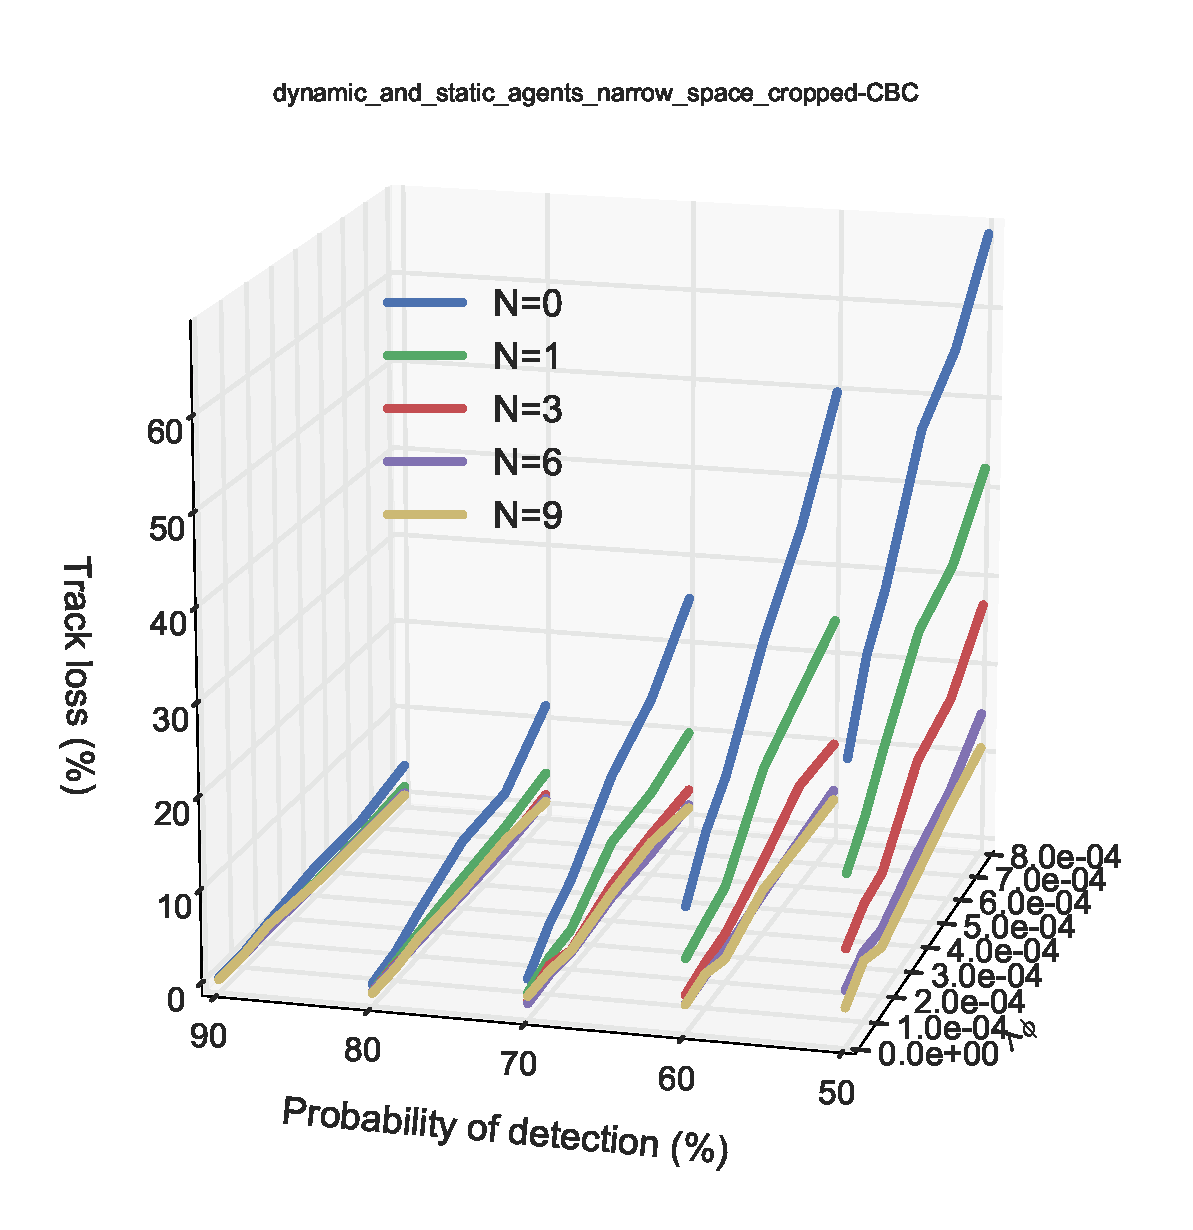
\includegraphics[width=\textwidth]{dynamic_and_static_agents_narrow_space_cropped-CBC}
        \caption{CBC solver}
    \end{subfigure}
    \begin{subfigure}{0.49\textwidth}
        \centering
        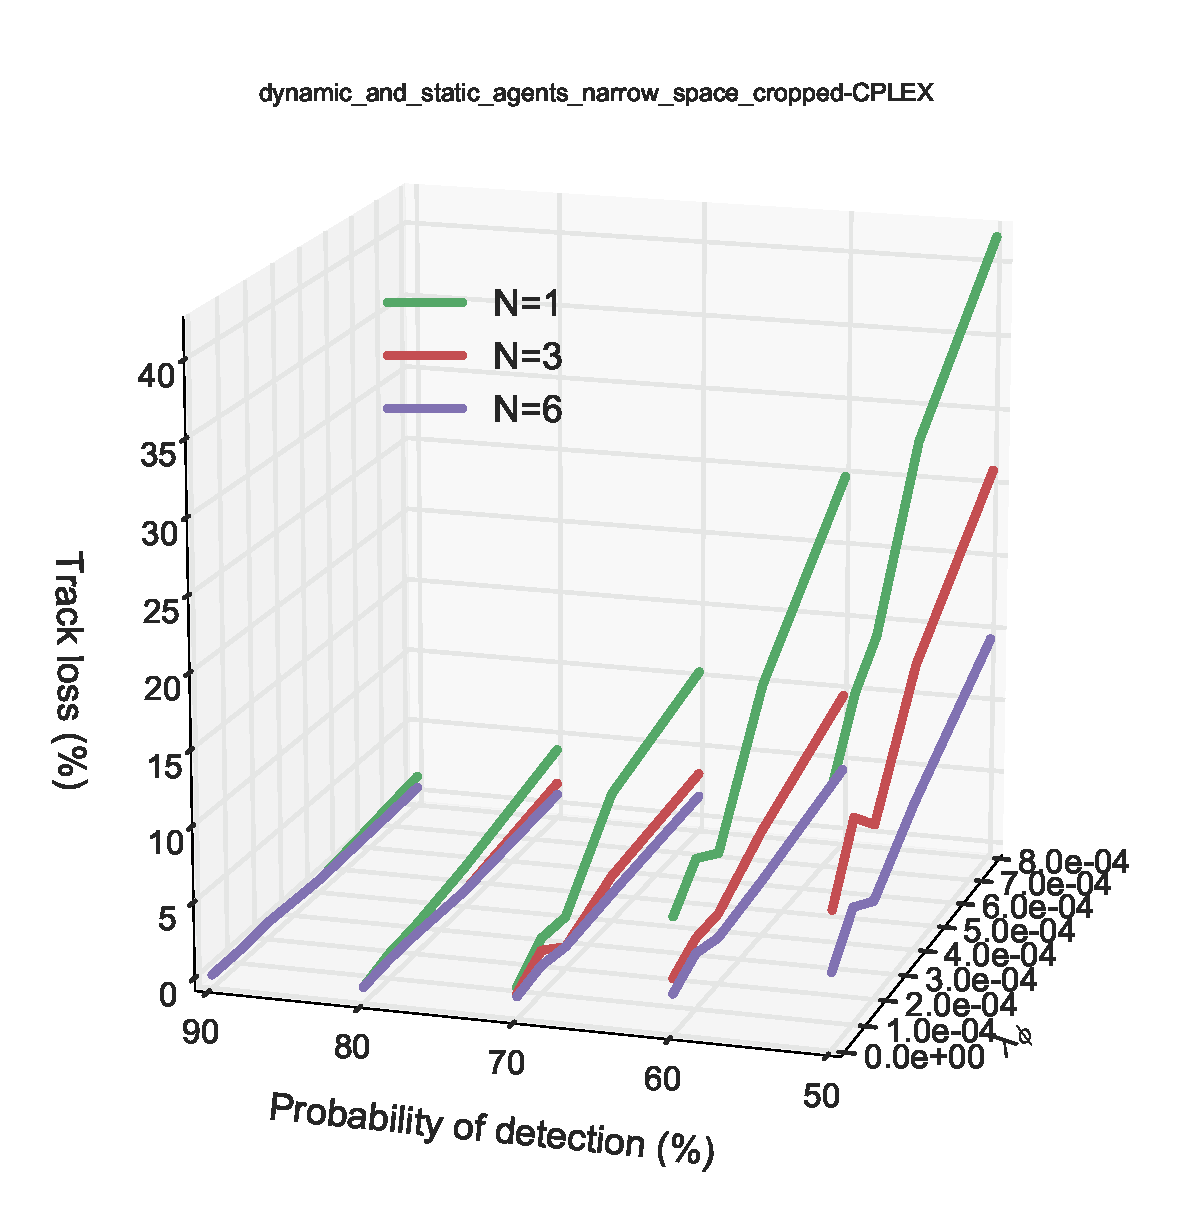
\includegraphics[width=\textwidth]{dynamic_and_static_agents_narrow_space_cropped-CPLEX}
        \caption{CPLEX solver}
    \end{subfigure}
    \begin{subfigure}{0.49\textwidth}
        \centering
        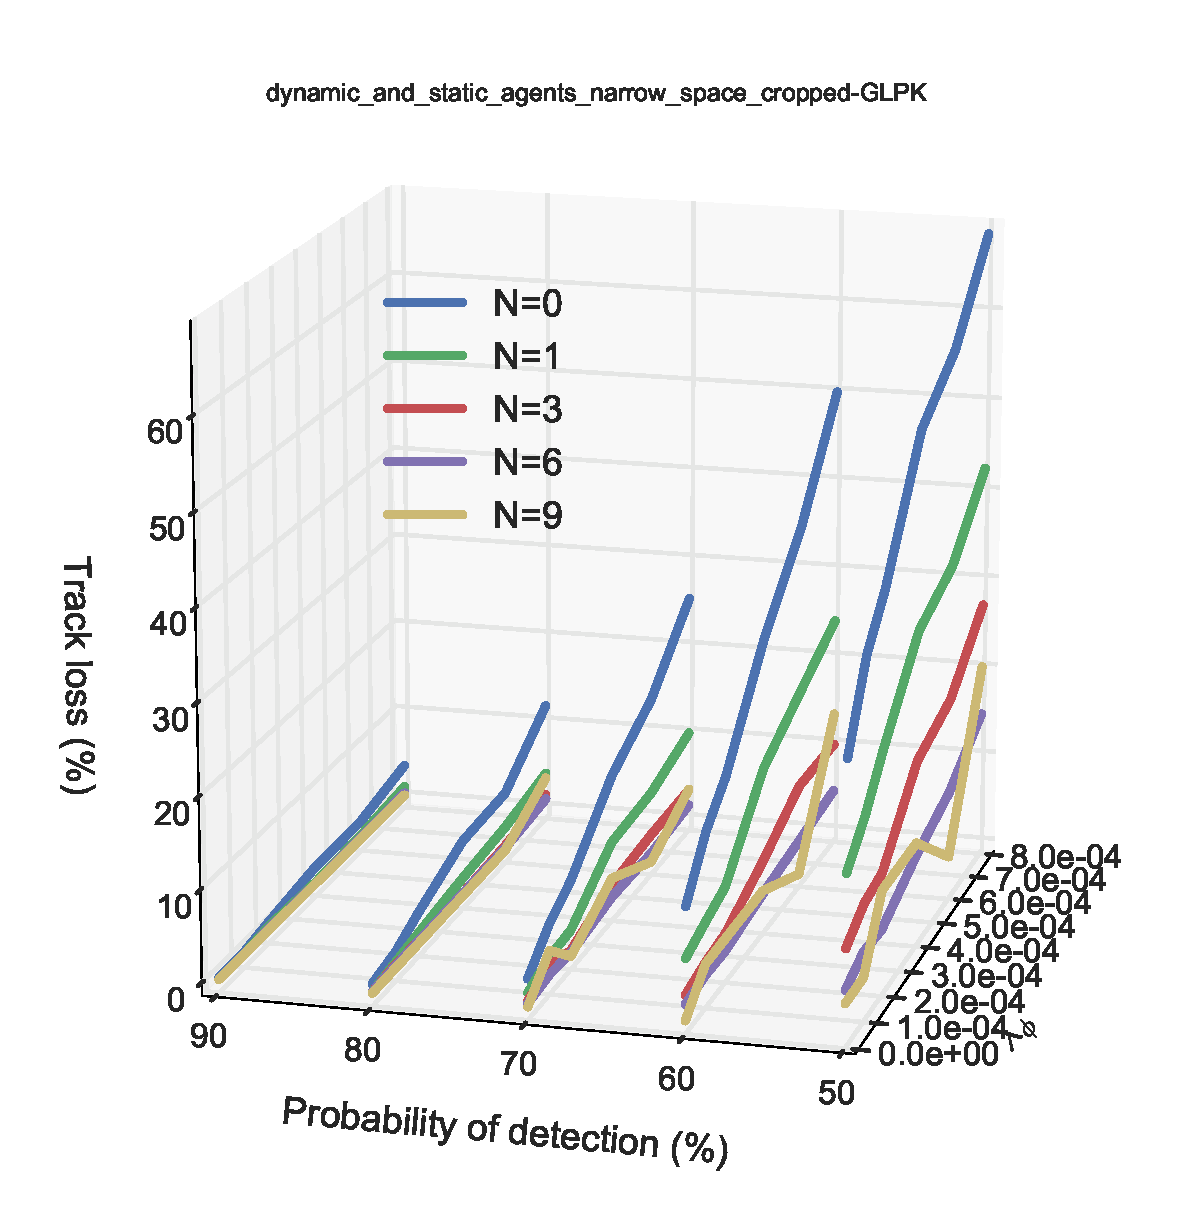
\includegraphics[width=\textwidth]{dynamic_and_static_agents_narrow_space_cropped-GLPK}
        \caption{GLPK solver}
    \end{subfigure}
    \begin{subfigure}{0.49\textwidth}
        \centering
        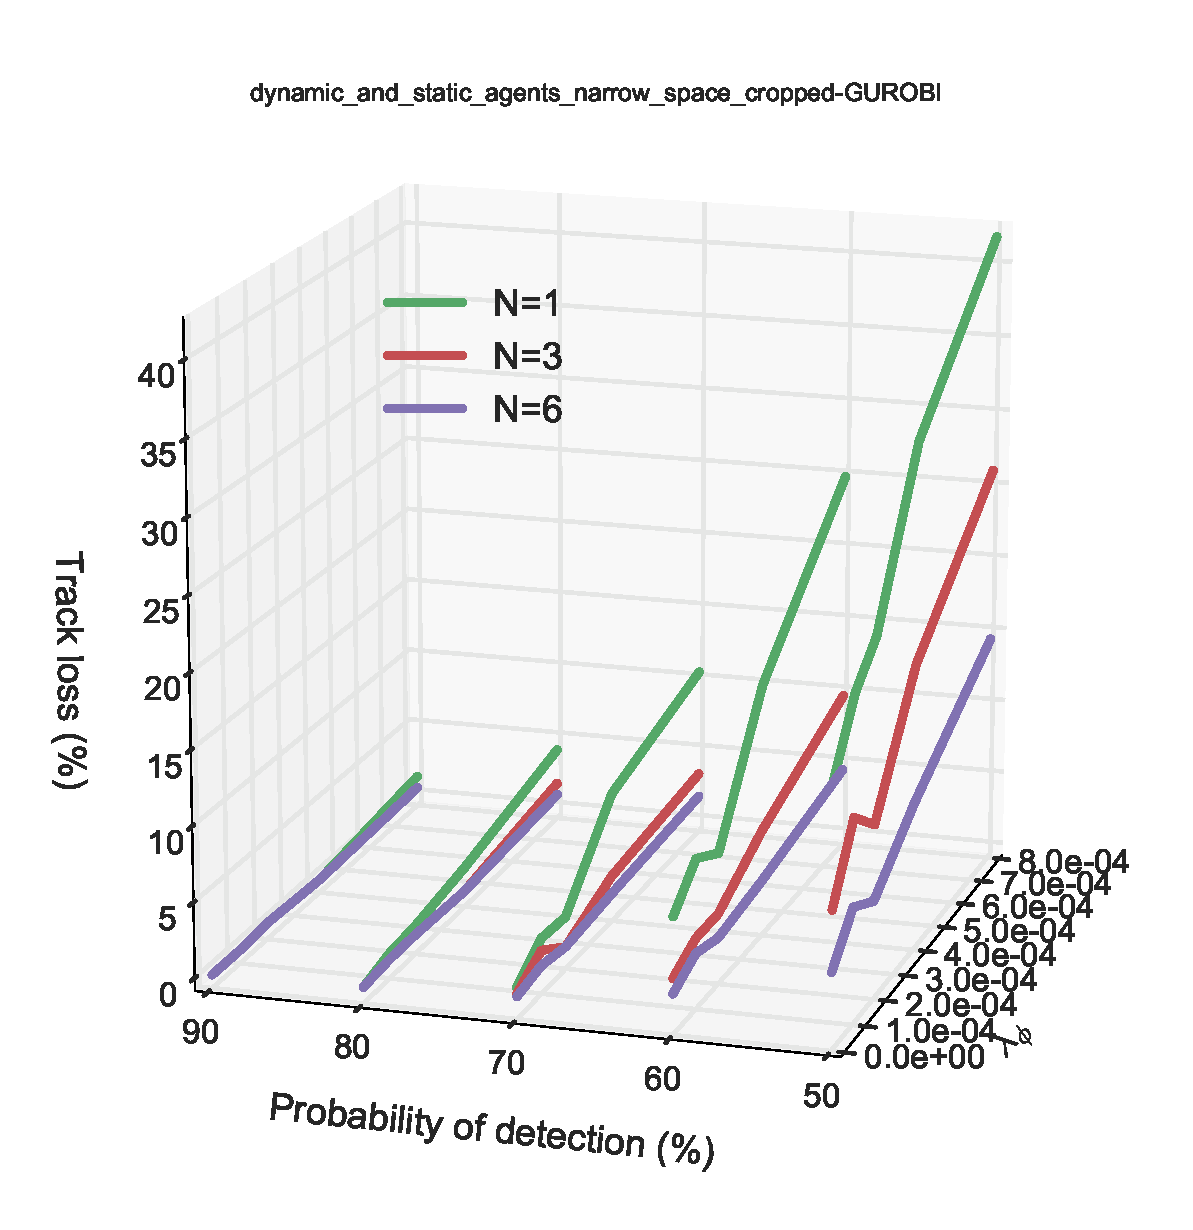
\includegraphics[width=\textwidth]{dynamic_and_static_agents_narrow_space_cropped-GUROBI}
        \caption{GUROBI solver}
    \end{subfigure}
    \caption{Simulation results for all solvers in scenario 4}
	\label{fig:dynamic_and_static_agents_narrow_space_cropped}
\end{figure}

\begin{figure}[H]
    \centering
    \textbf{Scenario 5 - Track performance}\par \medskip
    \begin{subfigure}{0.49\textwidth}
        \centering
        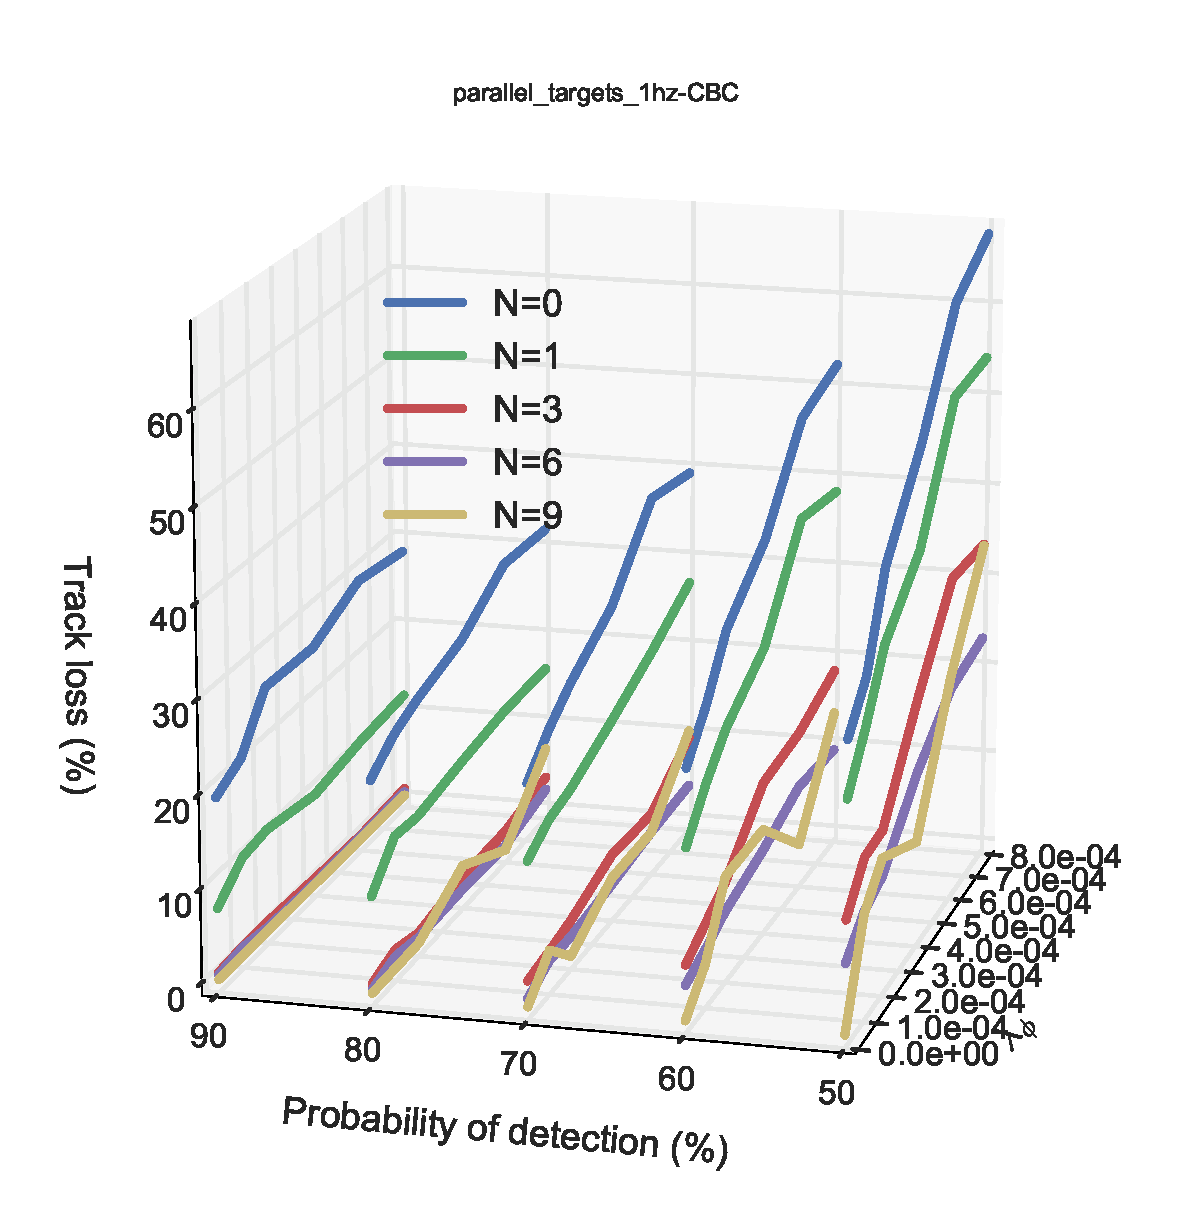
\includegraphics[width=\textwidth]{parallel_targets_1hz-CBC}
        \caption{CBC solver}
    \end{subfigure}
    \begin{subfigure}{0.49\textwidth}
        \centering
        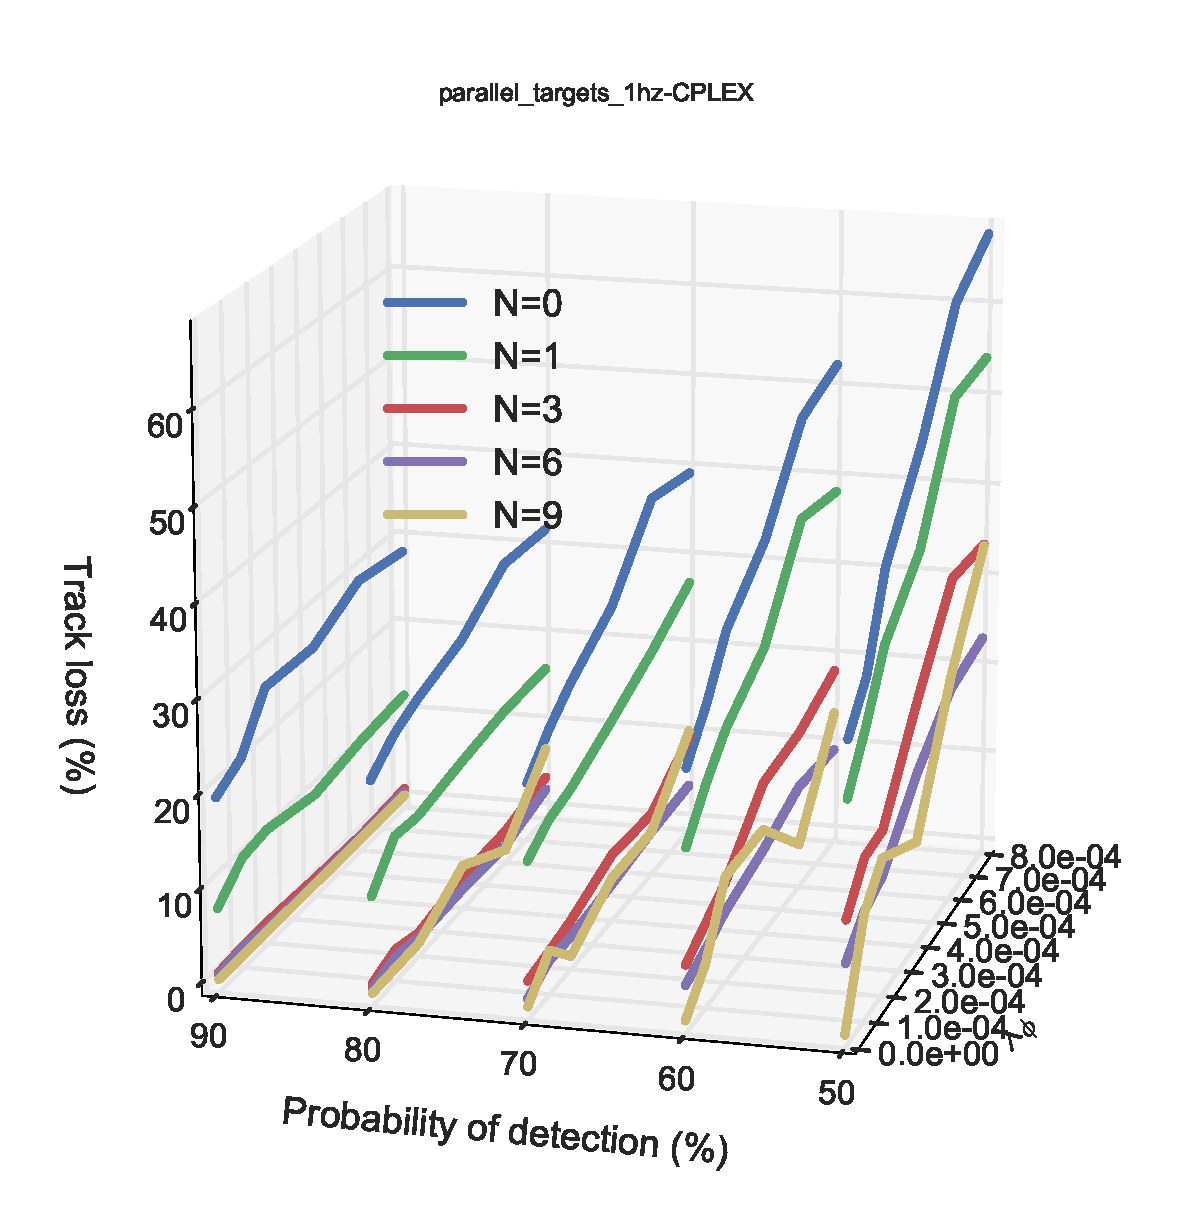
\includegraphics[width=\textwidth]{parallel_targets_1hz-CPLEX}
        \caption{CPLEX solver}
    \end{subfigure}
    \begin{subfigure}{0.49\textwidth}
        \centering
        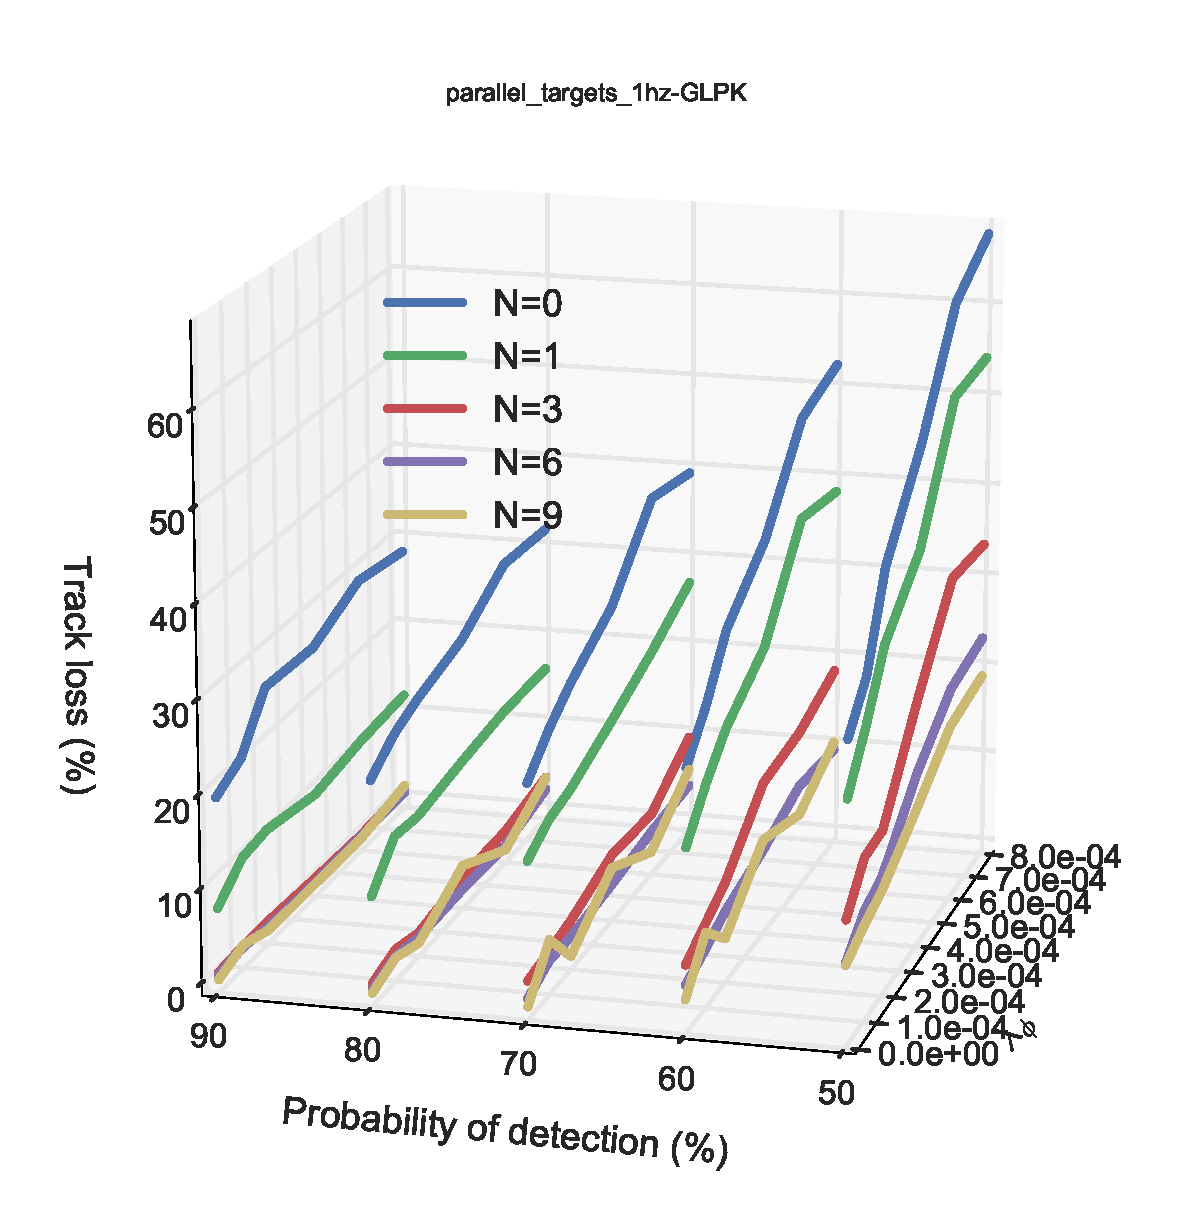
\includegraphics[width=\textwidth]{parallel_targets_1hz-GLPK}
        \caption{GLPK solver}
    \end{subfigure}
    \begin{subfigure}{0.49\textwidth}
        \centering
        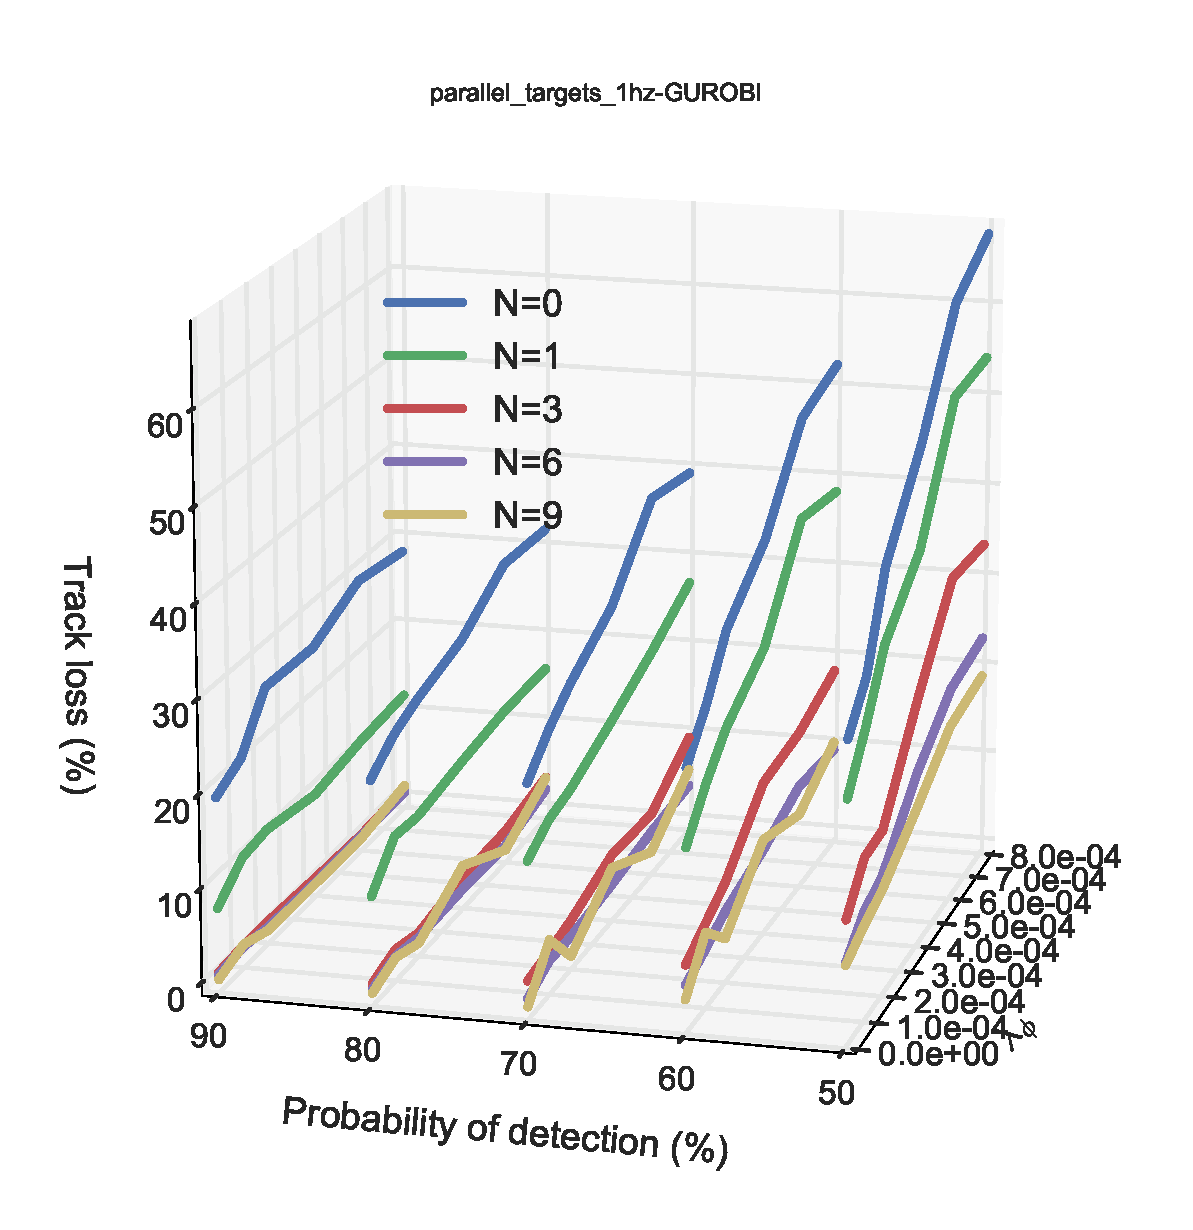
\includegraphics[width=\textwidth]{parallel_targets_1hz-GUROBI}
        \caption{GUROBI solver}
    \end{subfigure}
    \caption{Simulation results for all solvers in scenario 5}
    \label{fig:parallel_targets_1hz}
\end{figure} 

\begin{figure}[H]
    \centering
    \textbf{Scenario 6 - Track performance}\par \medskip
    \begin{subfigure}{0.49\textwidth}
        \centering
        \includegraphics[width=\textwidth]{{parallel_targets_0.5hz-CBC}.pdf}
        \caption{CBC solver}
    \end{subfigure}
    \begin{subfigure}{0.49\textwidth}
        \centering
        \includegraphics[width=\textwidth]{{parallel_targets_0.5hz-CPLEX}.pdf}
        \caption{CPLEX solver}
    \end{subfigure}
    \begin{subfigure}{0.49\textwidth}
        \centering
        \includegraphics[width=\textwidth]{{parallel_targets_0.5hz-GLPK}.pdf}
        \caption{GLPK solver}
    \end{subfigure}
    \begin{subfigure}{0.49\textwidth}
        \centering
        \includegraphics[width=\textwidth]{{parallel_targets_0.5hz-GUROBI}.pdf}
        \caption{GUROBI solver}
    \end{subfigure}
    \caption{Simulation results for all solvers in scenario 6}
    \label{fig:parallel_targets_0.5hz}
\end{figure}
	
	\section{Parallel runtime on virtual server}
	%!TEX root = ../TTK4550-MHT.tex
\begin{table}[H]
\centering
\begin{tabular}{c c c c c c}
\bfseries Processes & \bfseries Total & \bfseries Grow & \bfseries Cluster & \bfseries Optimize & \bfseries Prune \\ \hline
\csvreader[head to column names]{{data/parallelTimeLog_AWS.csv}}{}
{\Processes & \Total & \Grow & \Cluster & \Optimize & \Prune \\\hline}
\end{tabular}
\caption{Runtime of a scan with different amount of processes (time in ms)}	
\label{tab:runtime_parallel_aws}
\end{table}

\begin{table}[H]
\centering
\begin{tabular}{c c c c c}
\bfseries Processes & \bfseries Grow & \bfseries Cluster & \bfseries Optimize & \bfseries Prune \\ \hline
\csvreader[head to column names,respect percent=true]{{data/parallelTimeLogPercentage_AWS.csv}}{}
{\Processes & \Grow \% & \Cluster \% & \Optimize \% & \Prune \% \\\hline }
\end{tabular}
\caption{Runtime distribution percentage}	
\label{tab:runtime_parallel_percentage_aws}
\end{table}

\begin{table}[H]
\centering
\begin{tabular}{c c c c c}
\bfseries Processes & \bfseries Search & \bfseries Predict & \bfseries Create & \bfseries Add \\ \hline
\csvreader[head to column names,respect percent=true]{{data/parallelTimeLogDistribution_AWS.csv}}{}
{\Processes & \Search \% & \Predict \% & \Create \% & \Add \% \\\hline }
\end{tabular}
\caption{Worker runtime distribution percentage}	
\label{tab:worker_parallel_percentage_aws}
\end{table}
%	\section{Run time plots}
%	%!TEX root = ../TTK4550-MHT.tex
\begin{figure}[H]
	\centering
	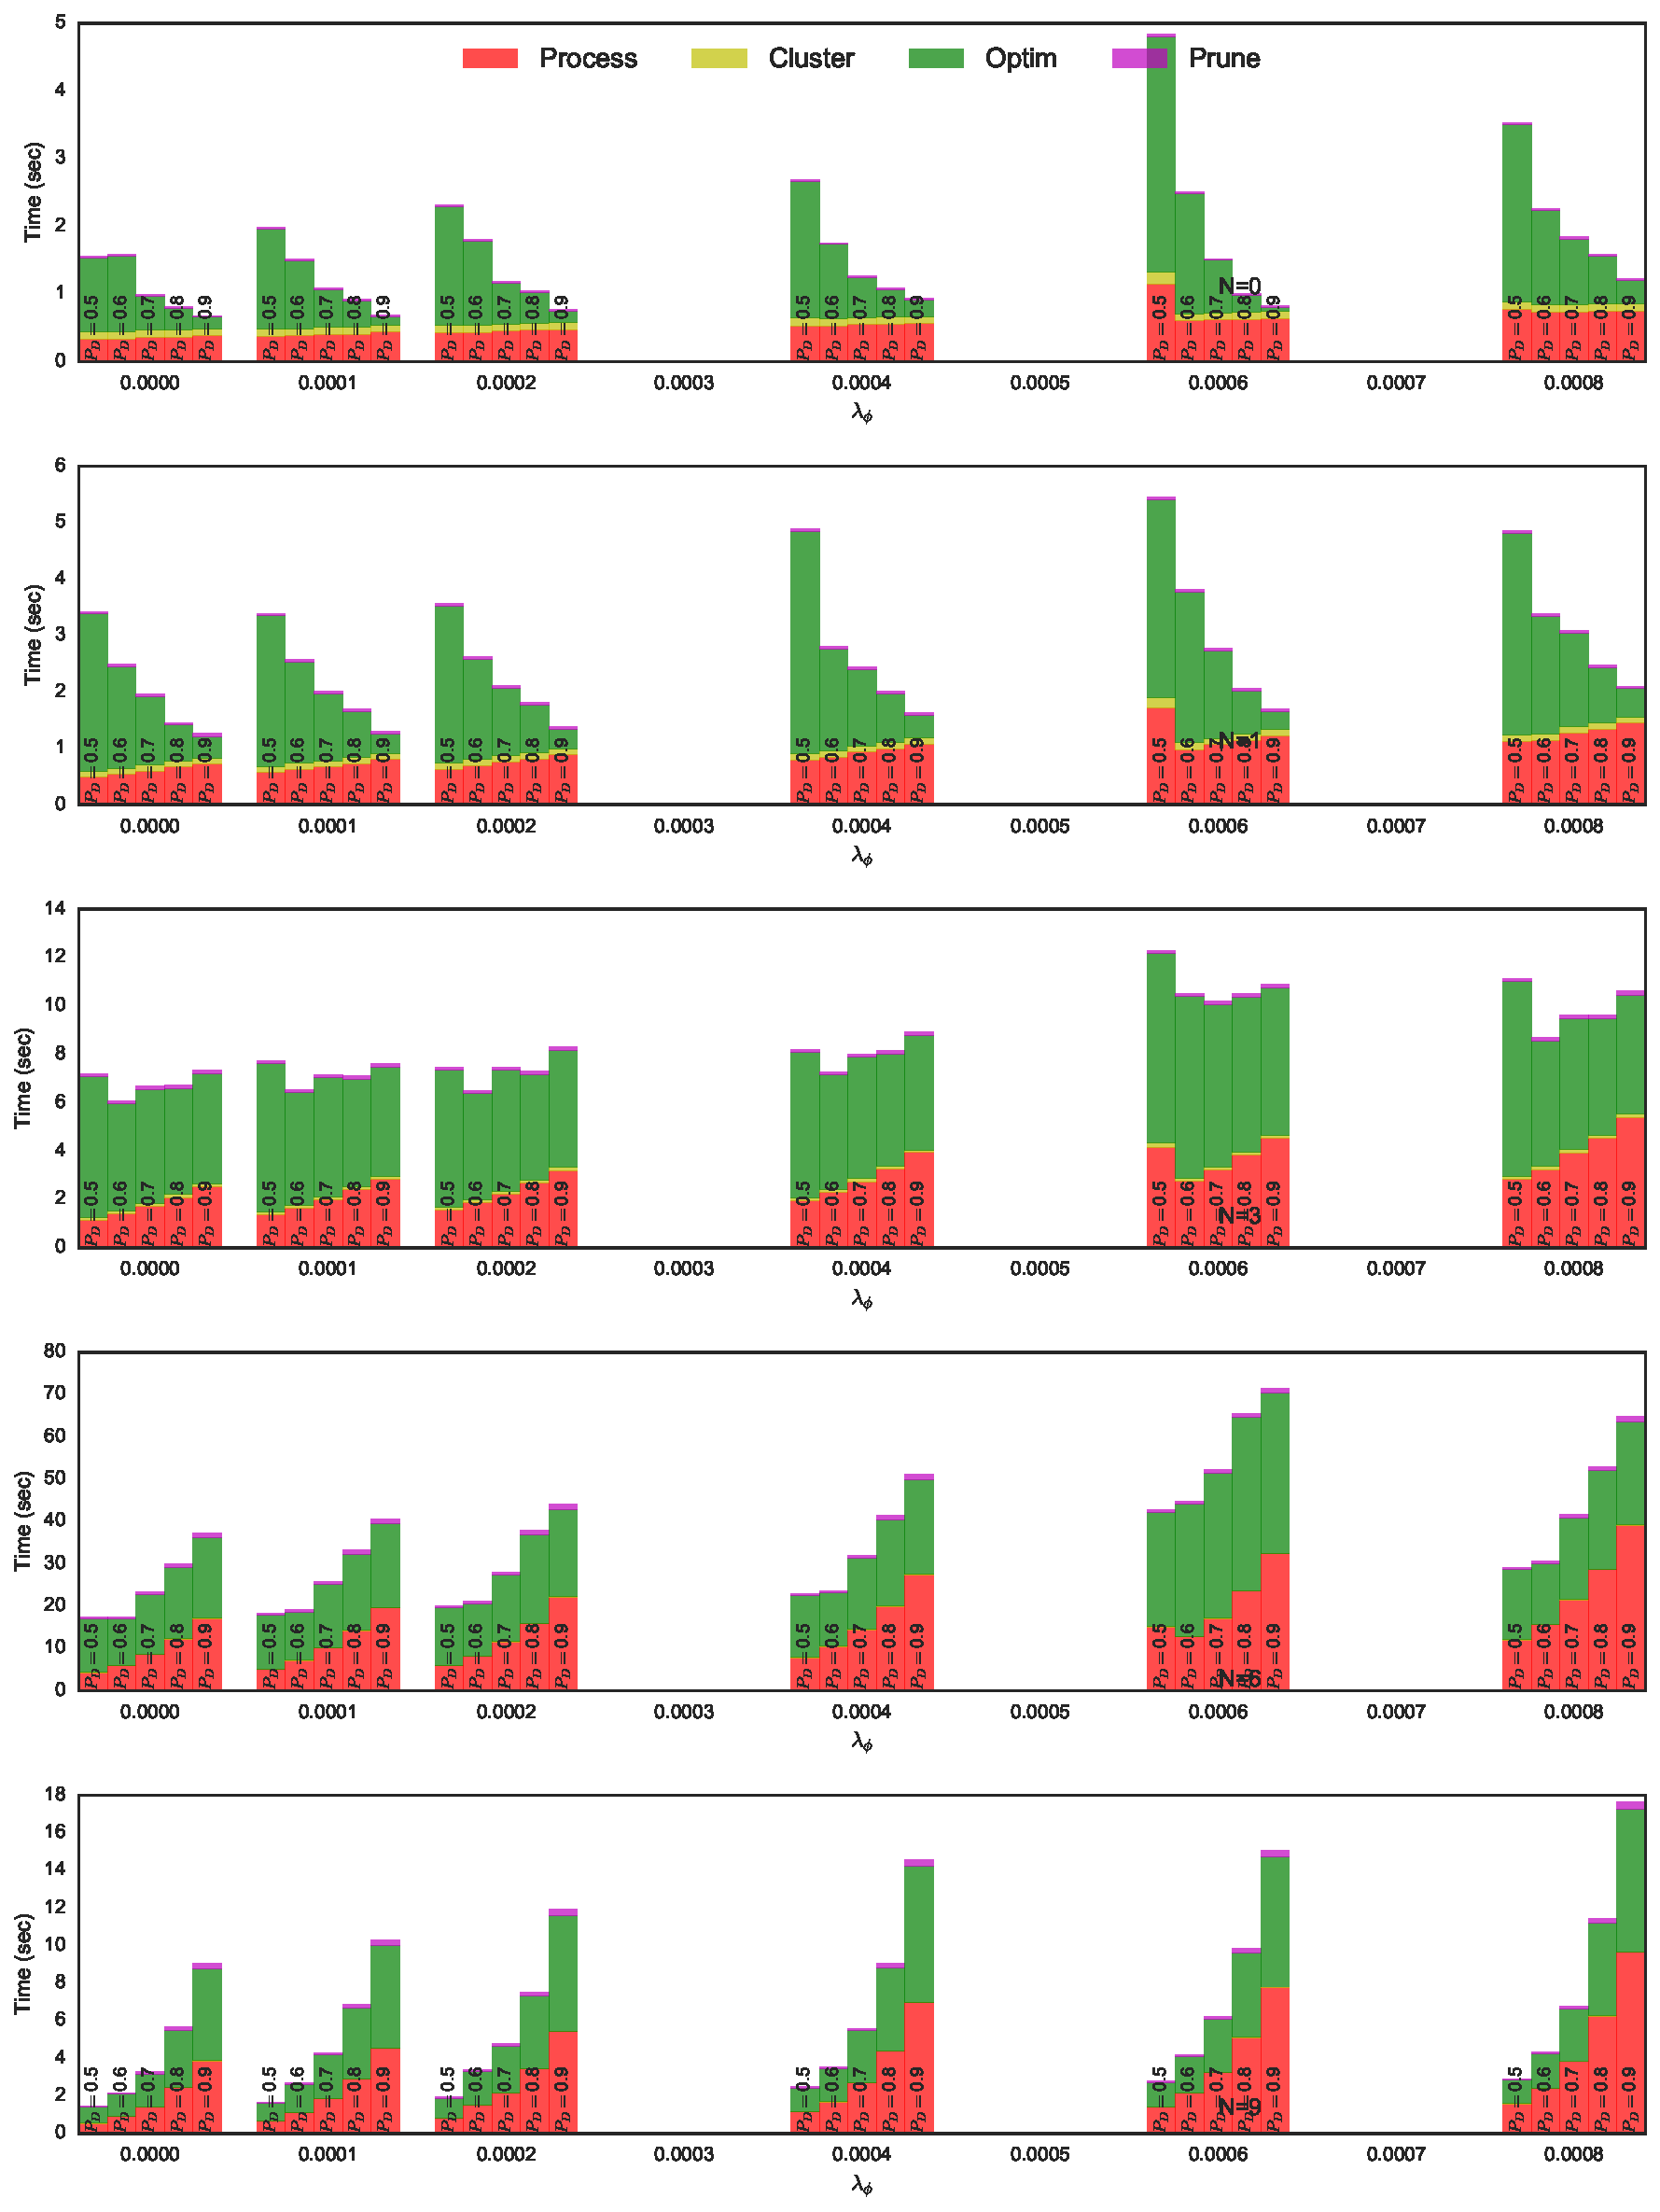
\includegraphics[width=\textwidth]{dynamic_agents_full_cooperation_cropped-CBC_runtimeLog}
	\caption{Scenario 1 - Run time log, CBC solver}
	\label{fig:runtimelog_scenario1-CBC}
\end{figure}
\begin{figure}[H]
	\centering
	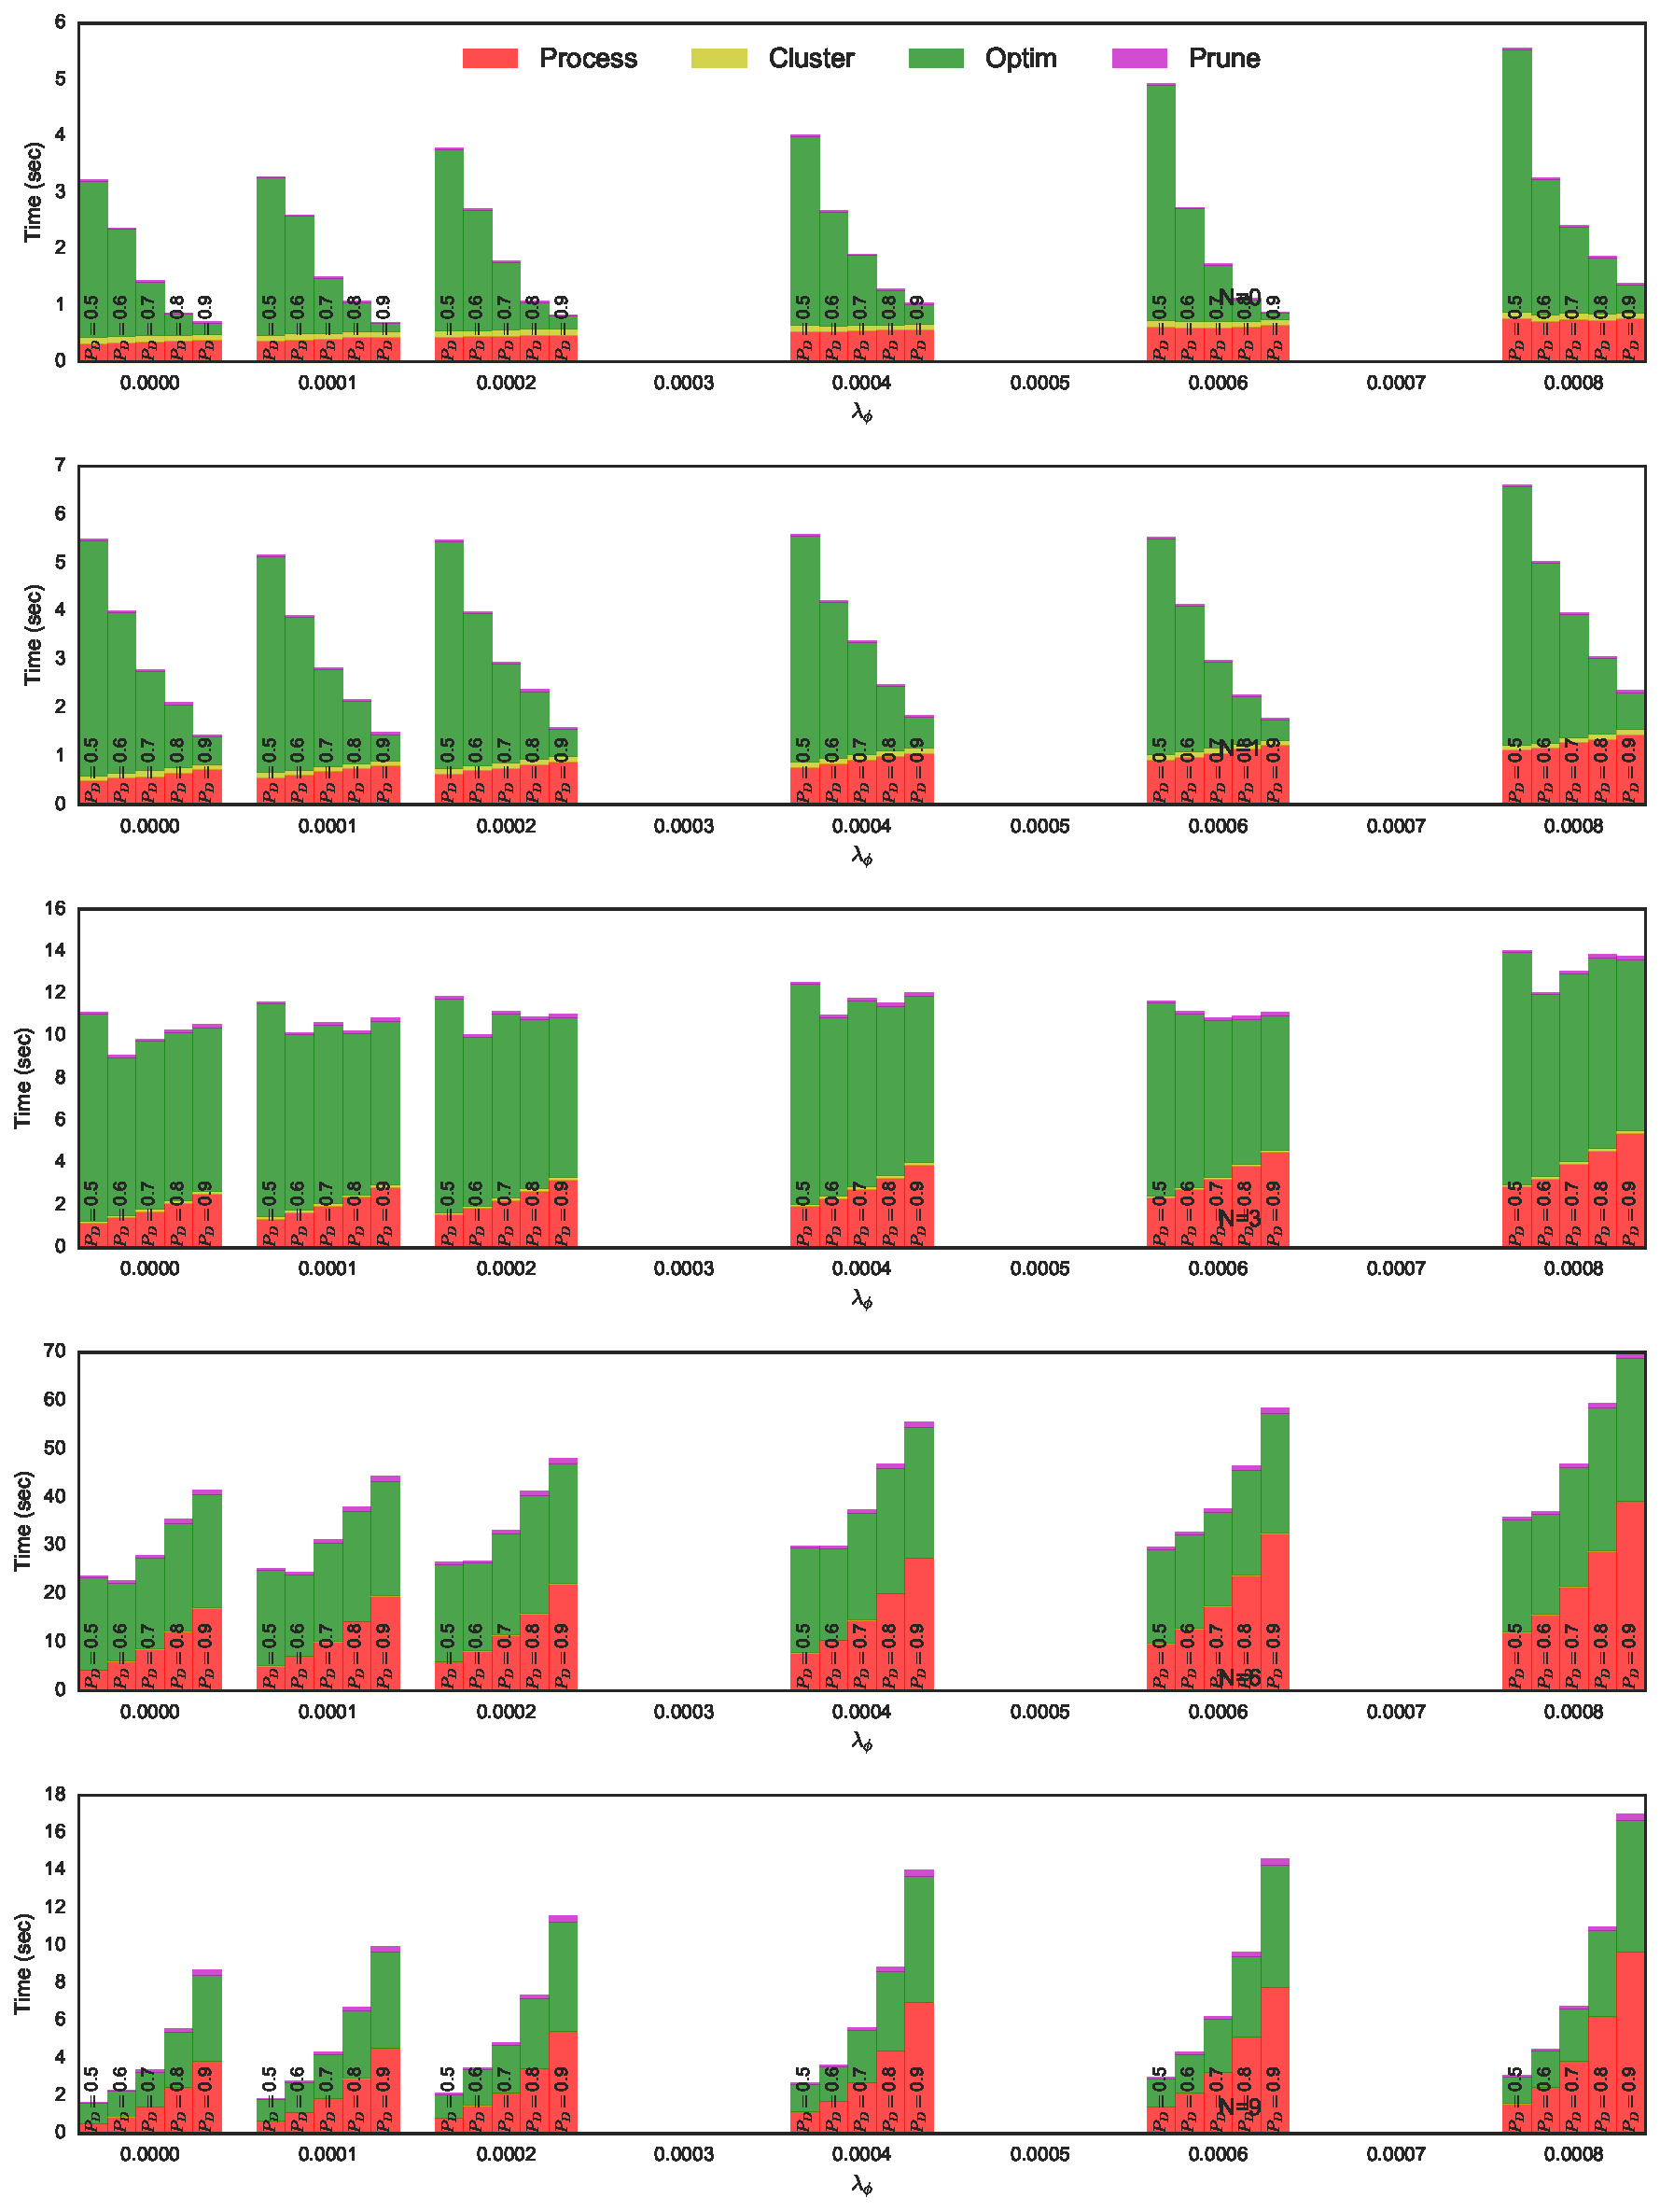
\includegraphics[width=\textwidth]{dynamic_agents_full_cooperation_cropped-CPLEX_runtimeLog}
	\caption{Scenario 1 - Run time log, CPLEX solver}
	\label{fig:runtimelog_scenario1-CPLEX}
\end{figure}
\begin{figure}[H]
	\centering
	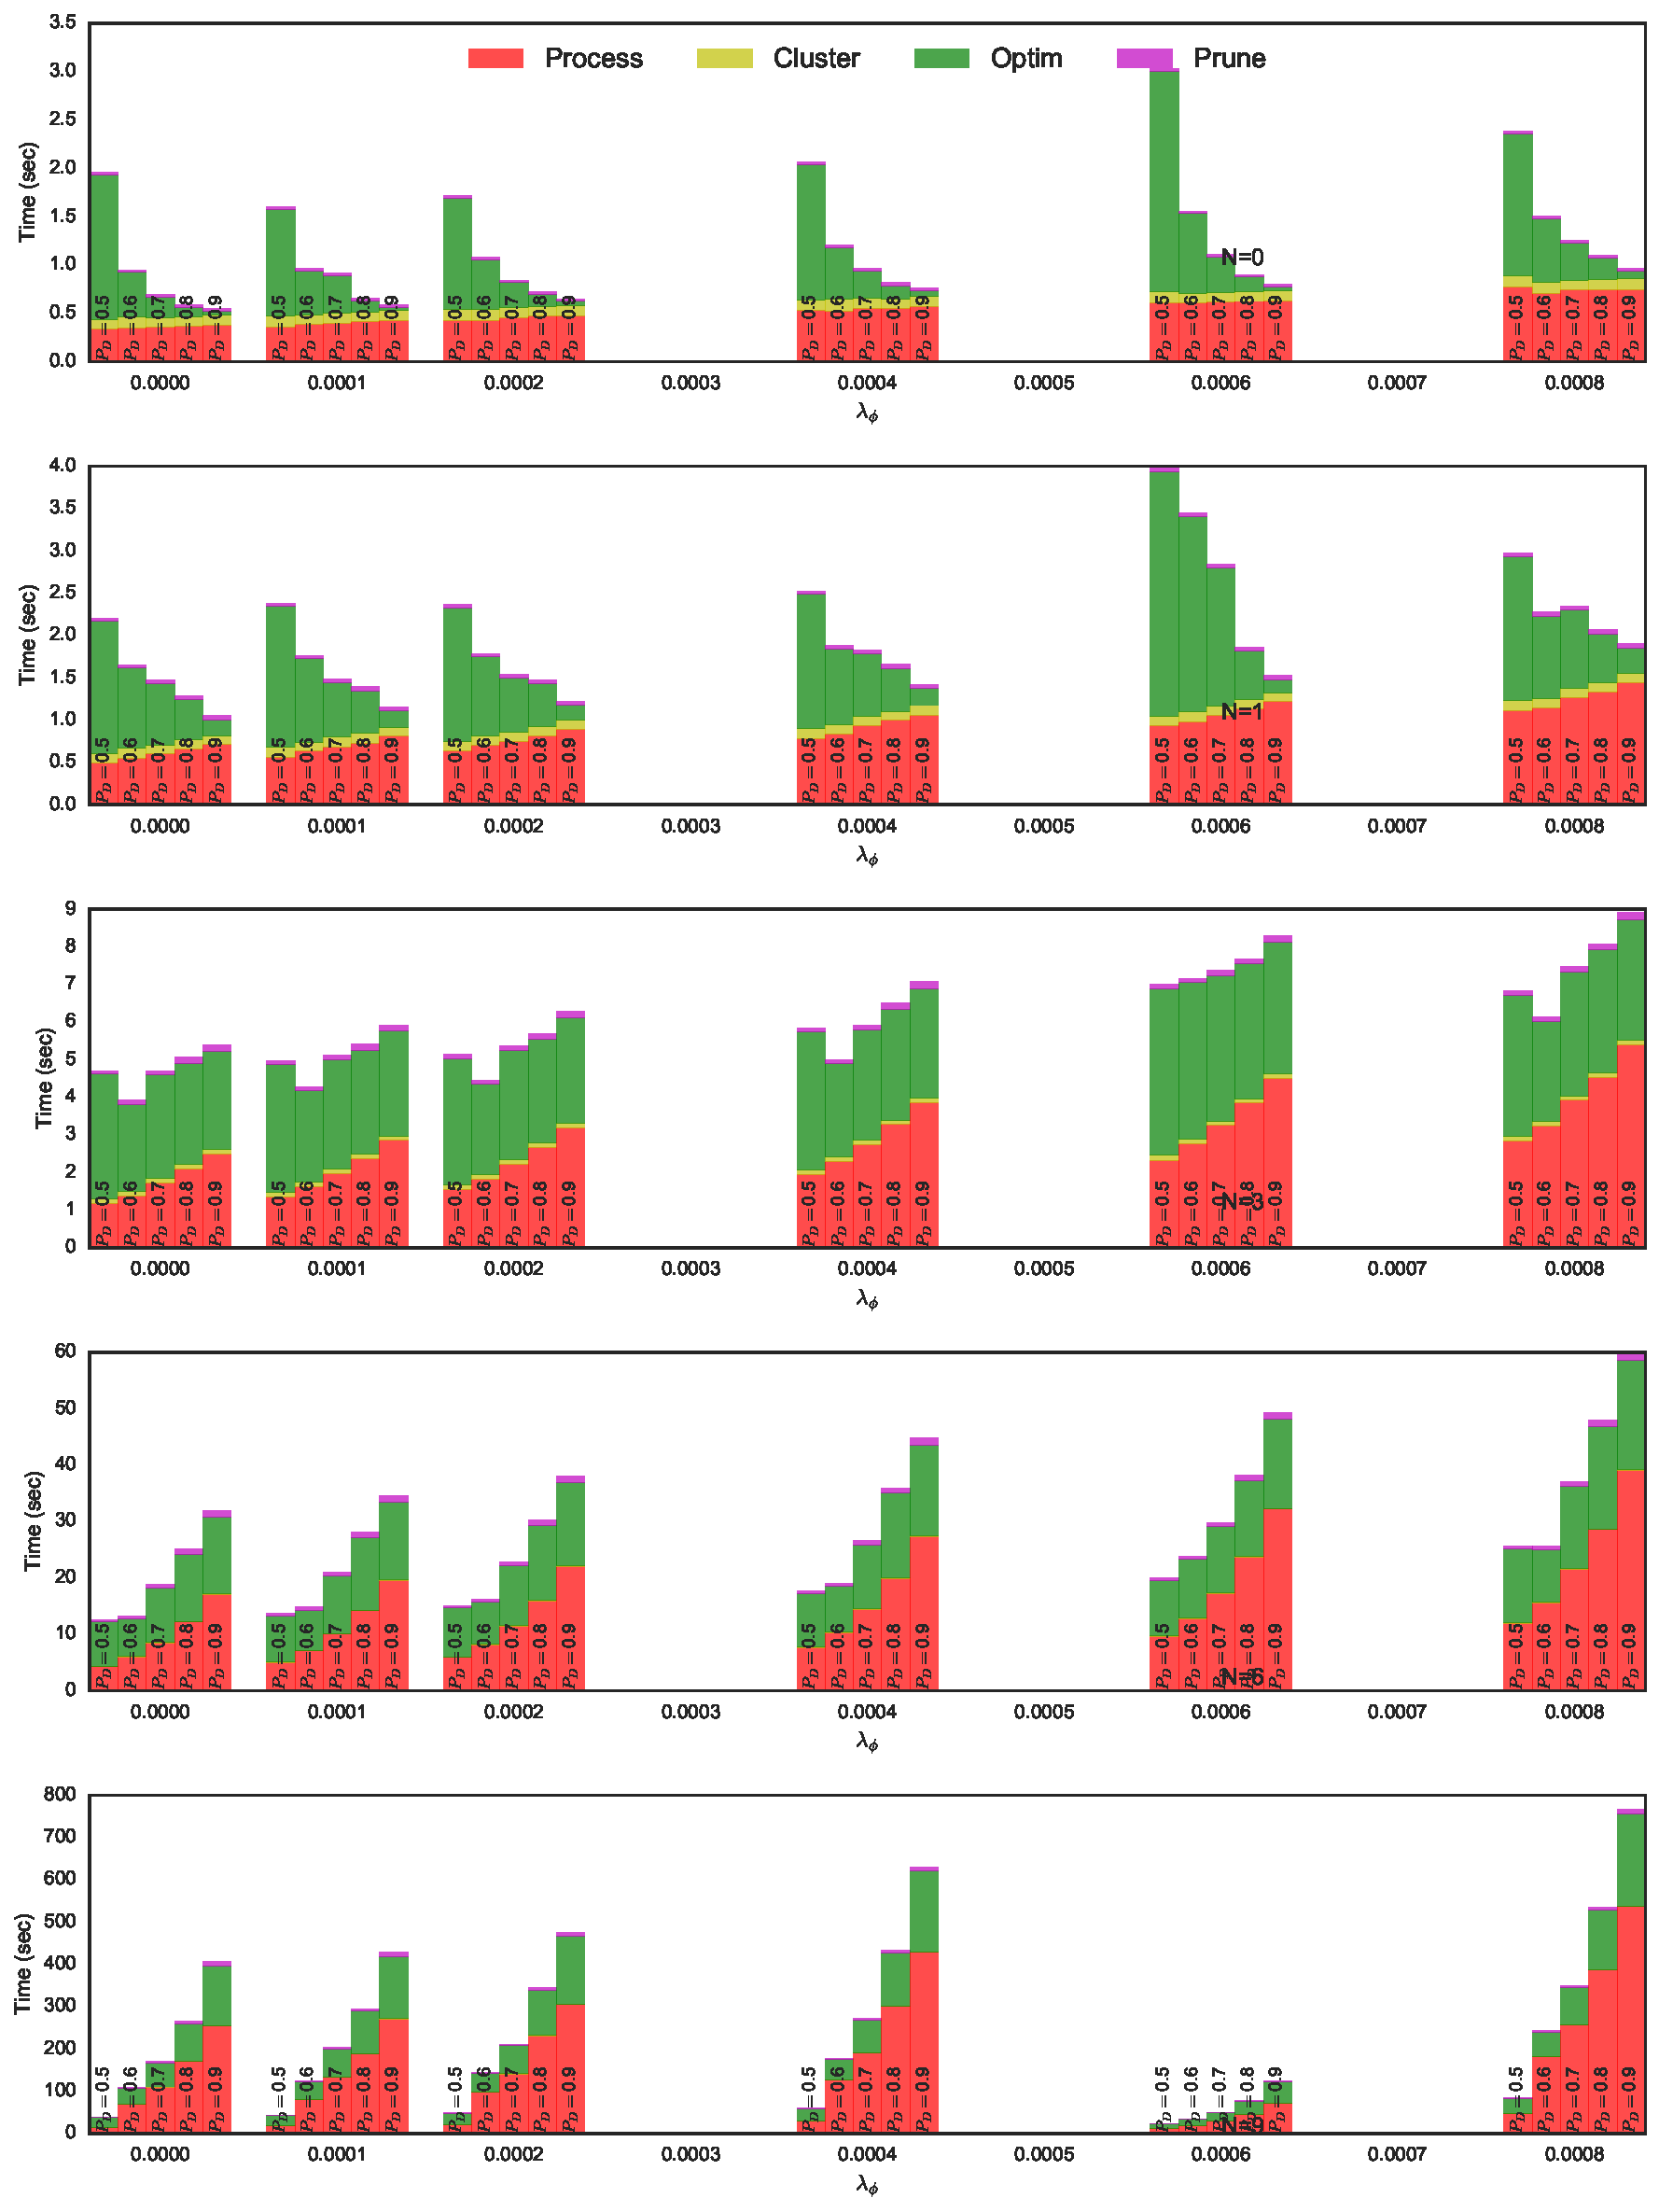
\includegraphics[width=\textwidth]{dynamic_agents_full_cooperation_cropped-GLPK_runtimeLog}
	\caption{Scenario 1 - Run time log, GLPK solver}
	\label{fig:runtimelog_scenario1-GLPK}
\end{figure}
\begin{figure}[H]
	\centering
	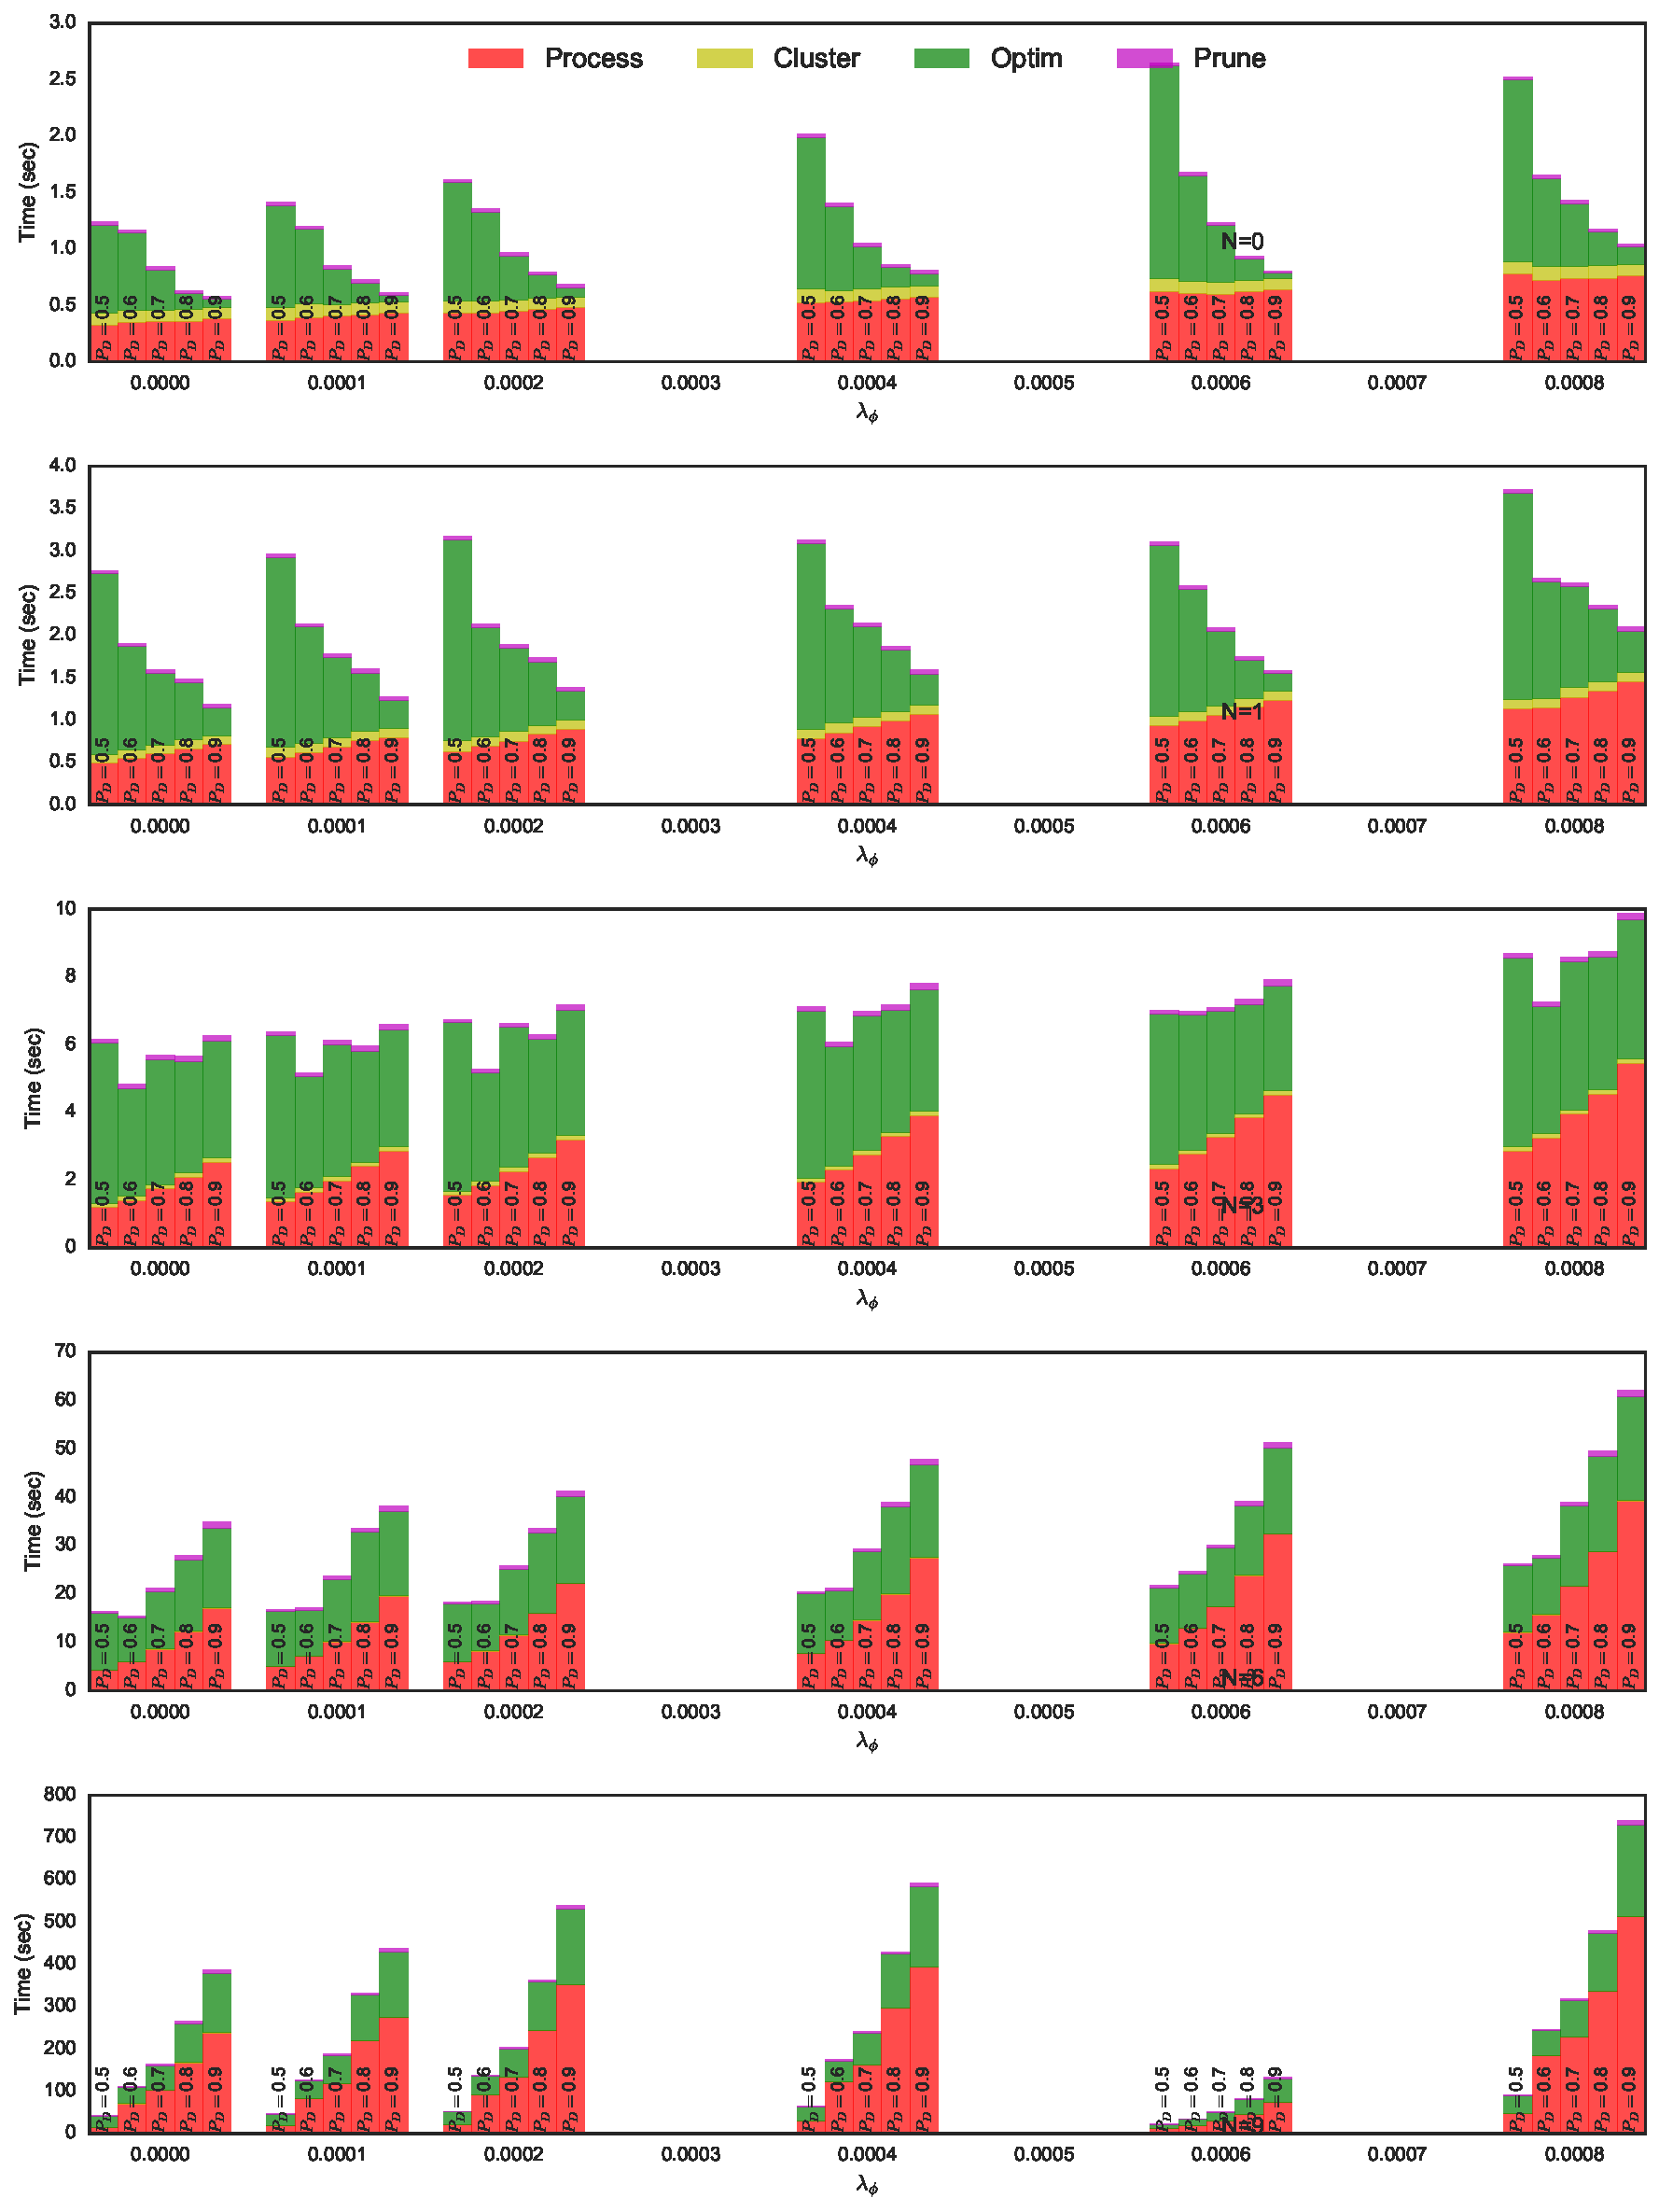
\includegraphics[width=\textwidth]{dynamic_agents_full_cooperation_cropped-GUROBI_runtimeLog}
	\caption{Scenario 1 - Run time log, GUROBI solver}
	\label{fig:runtimelog_scenario-GUROBI}
\end{figure}


\begin{figure}[H]
	\centering
	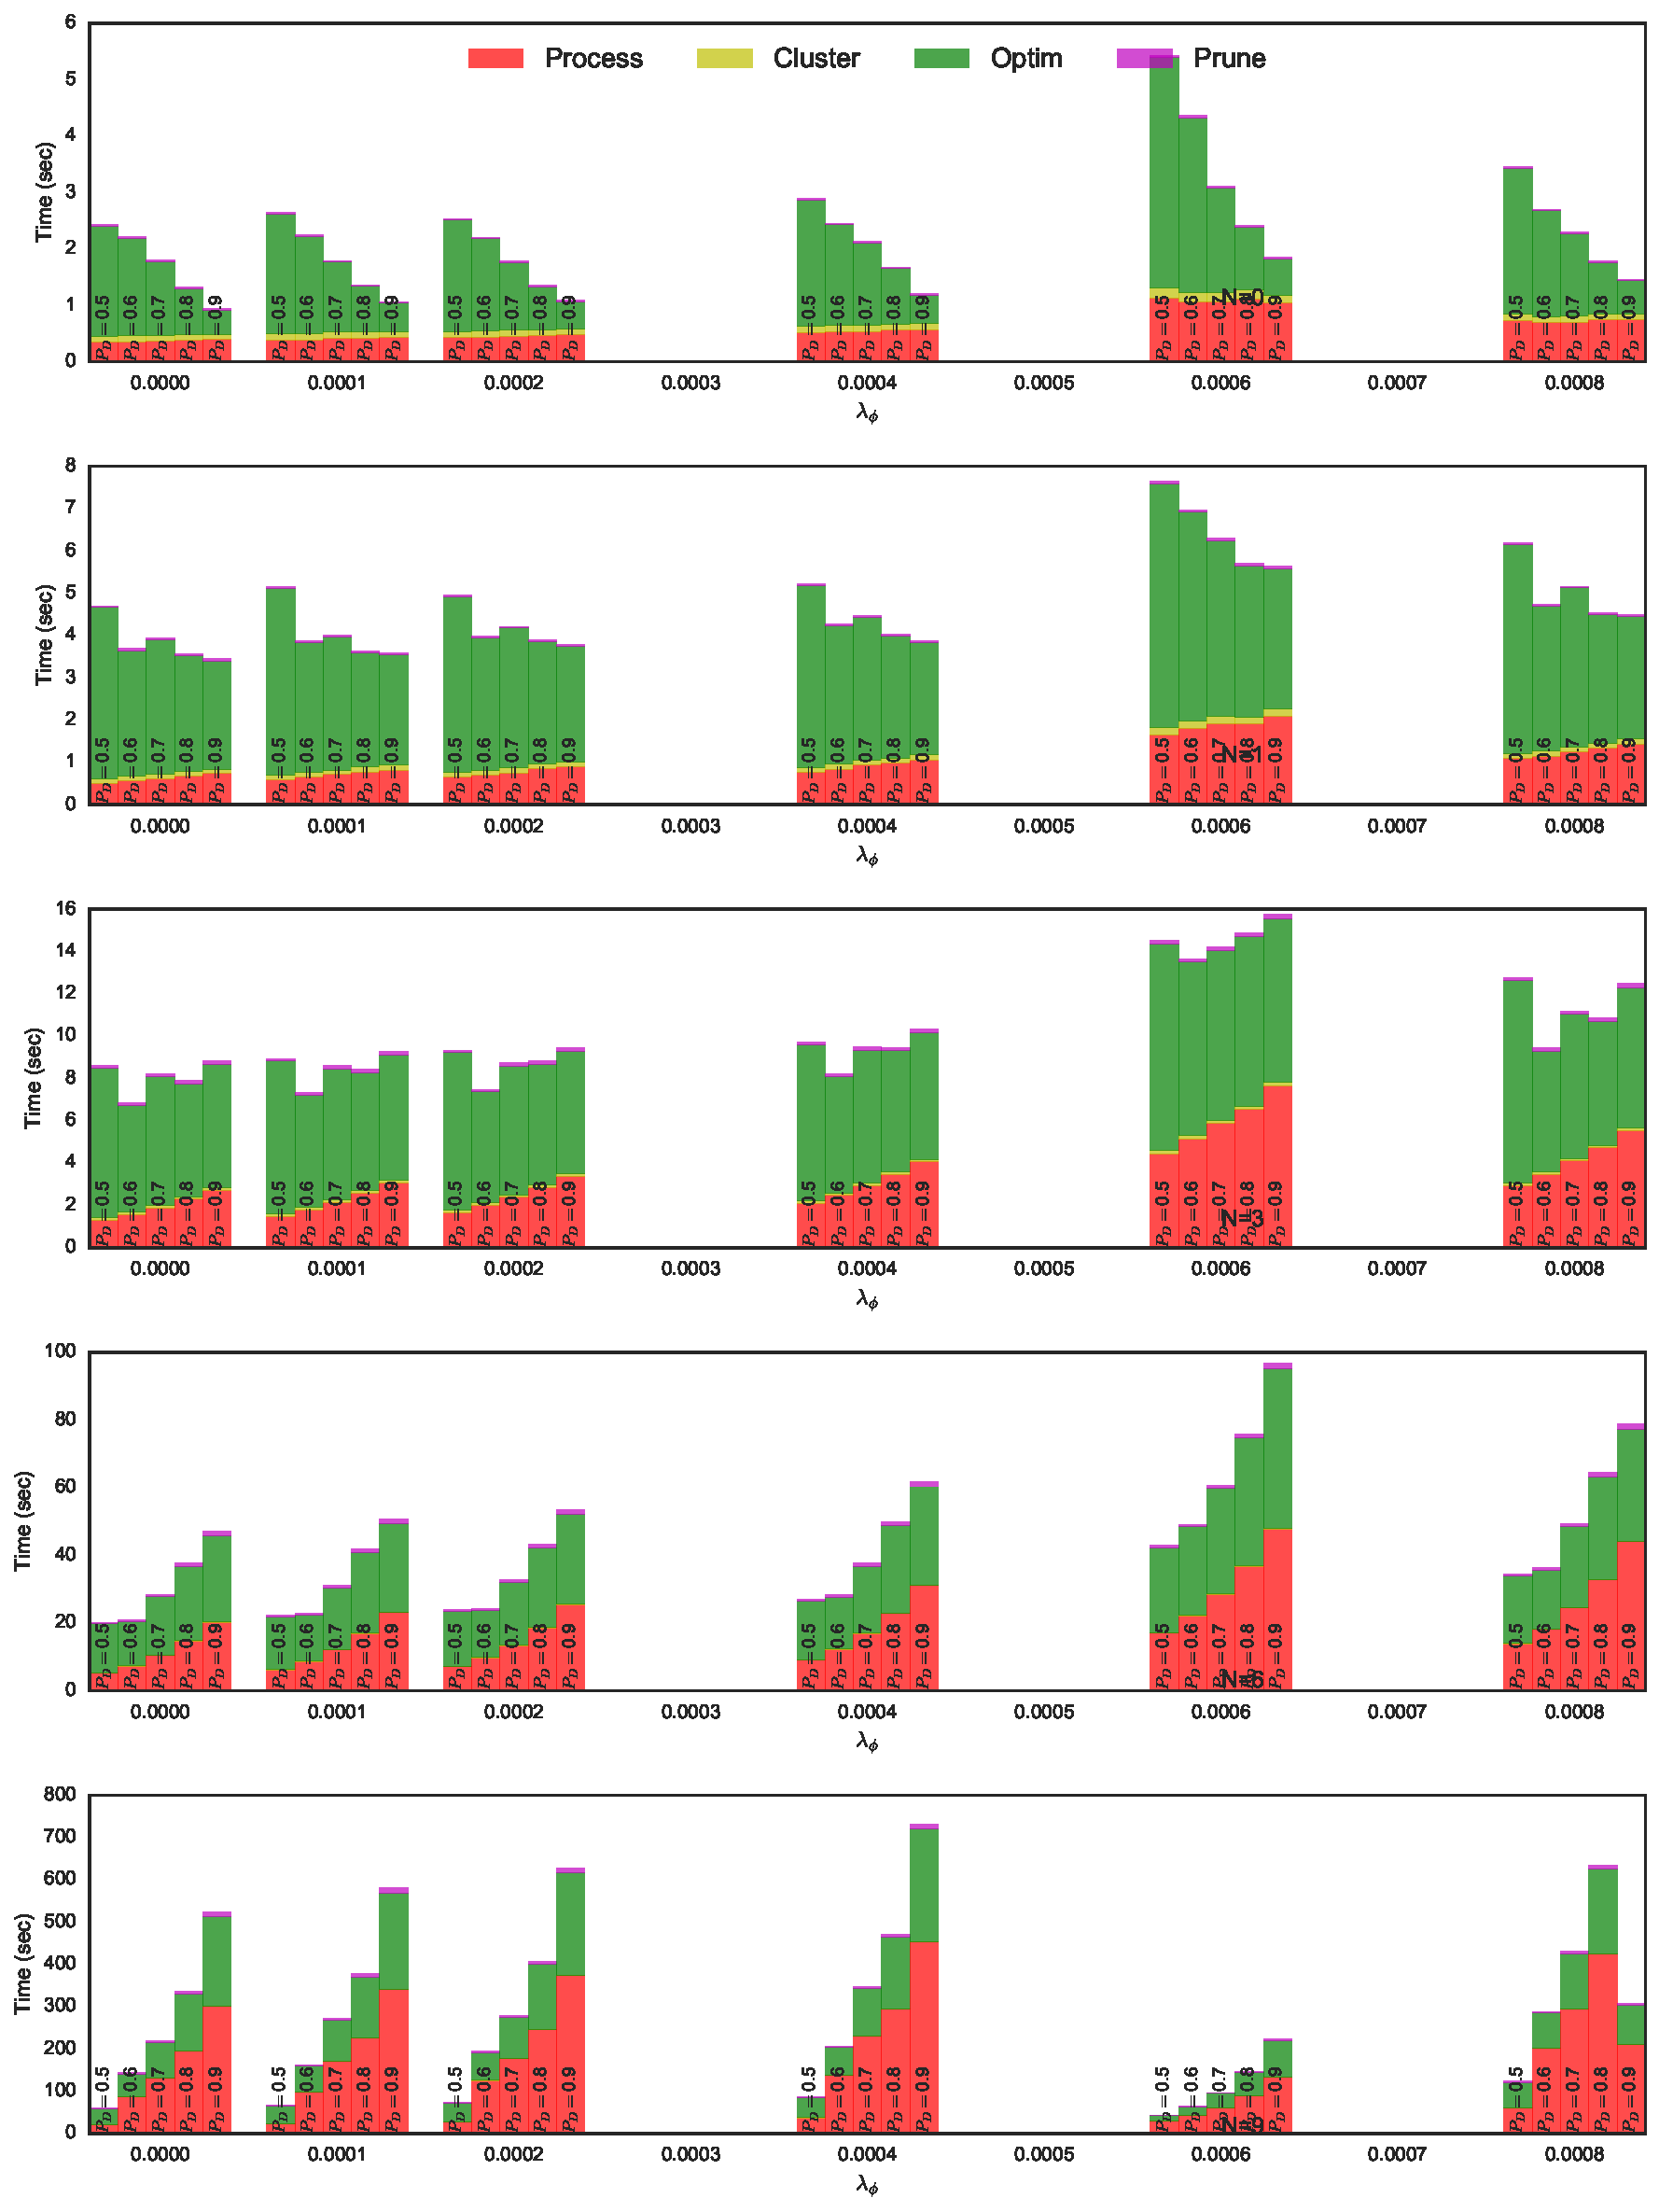
\includegraphics[width=\textwidth]{dynamic_agents_partial_cooporation_cropped-CBC_runtimeLog}
	\caption{Scenario 2 - Run time log, CBC solver}
	\label{fig:runtimelog_scenario2-CBC}
\end{figure}\begin{figure}[H]
	\centering
	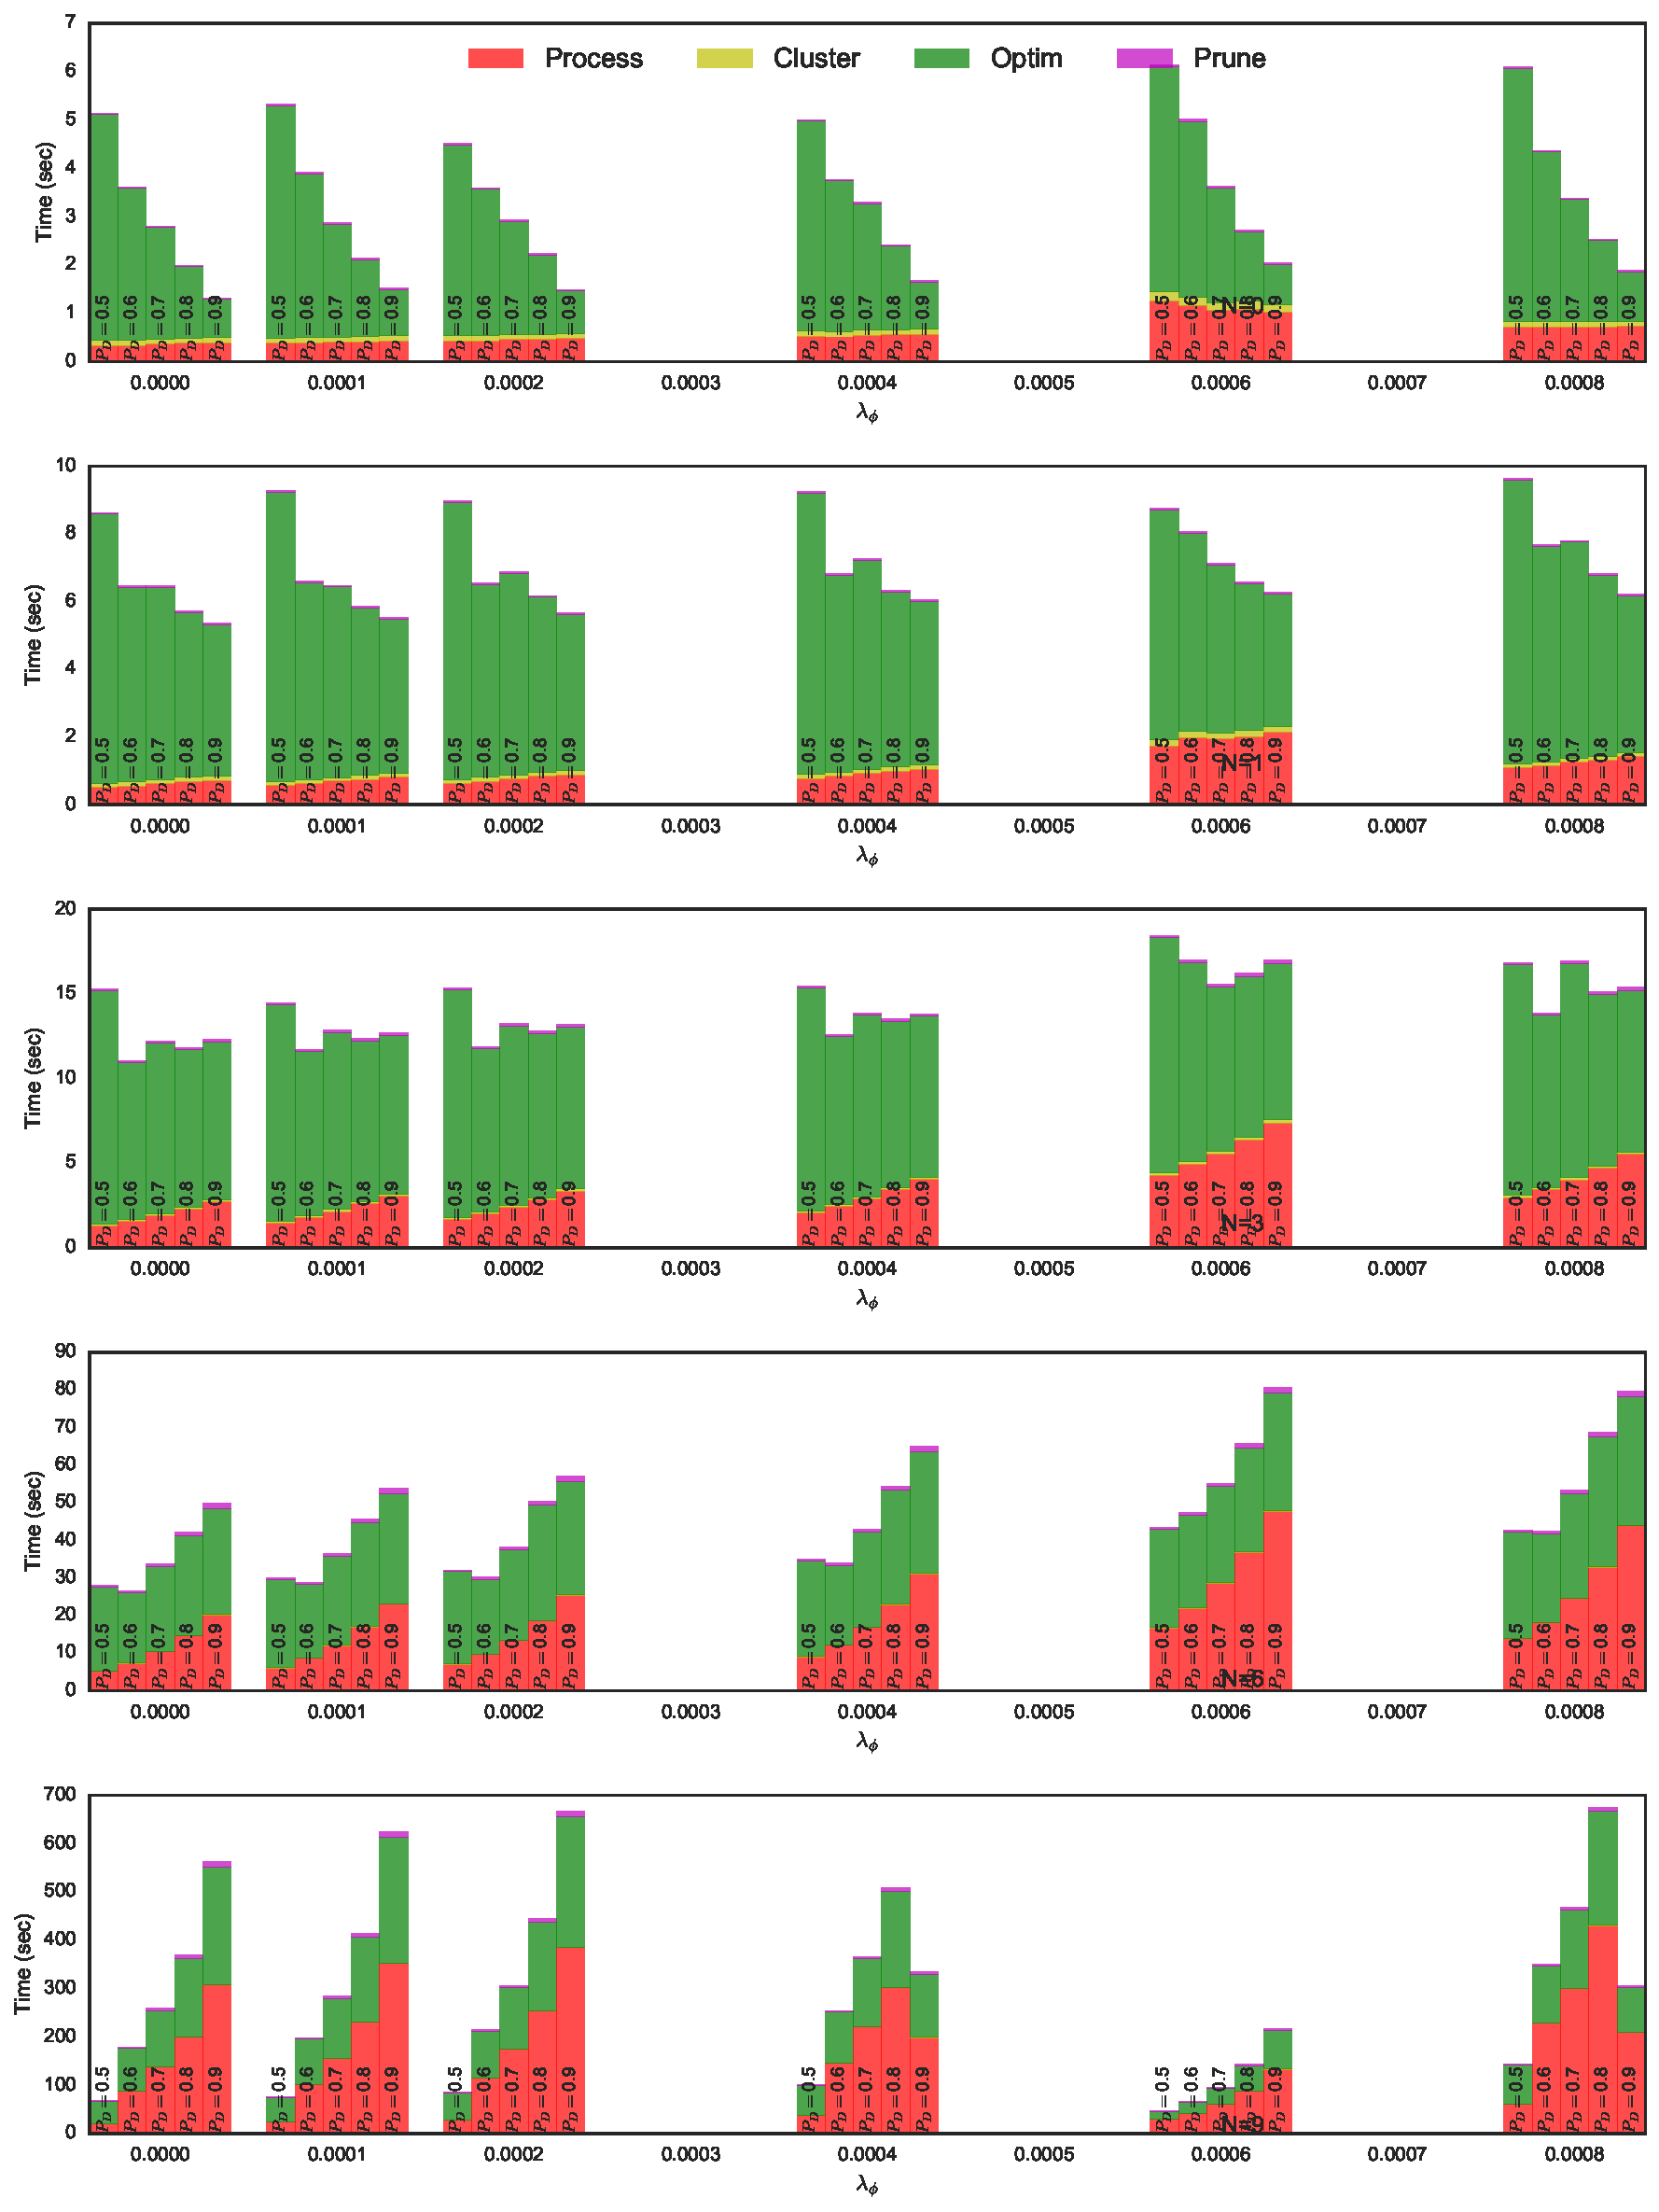
\includegraphics[width=\textwidth]{dynamic_agents_partial_cooporation_cropped-CPLEX_runtimeLog}
	\caption{Scenario 2 - Run time log, CPLEX solver}
	\label{fig:runtimelog_scenario2-CPLEX}
\end{figure}\begin{figure}[H]
	\centering
	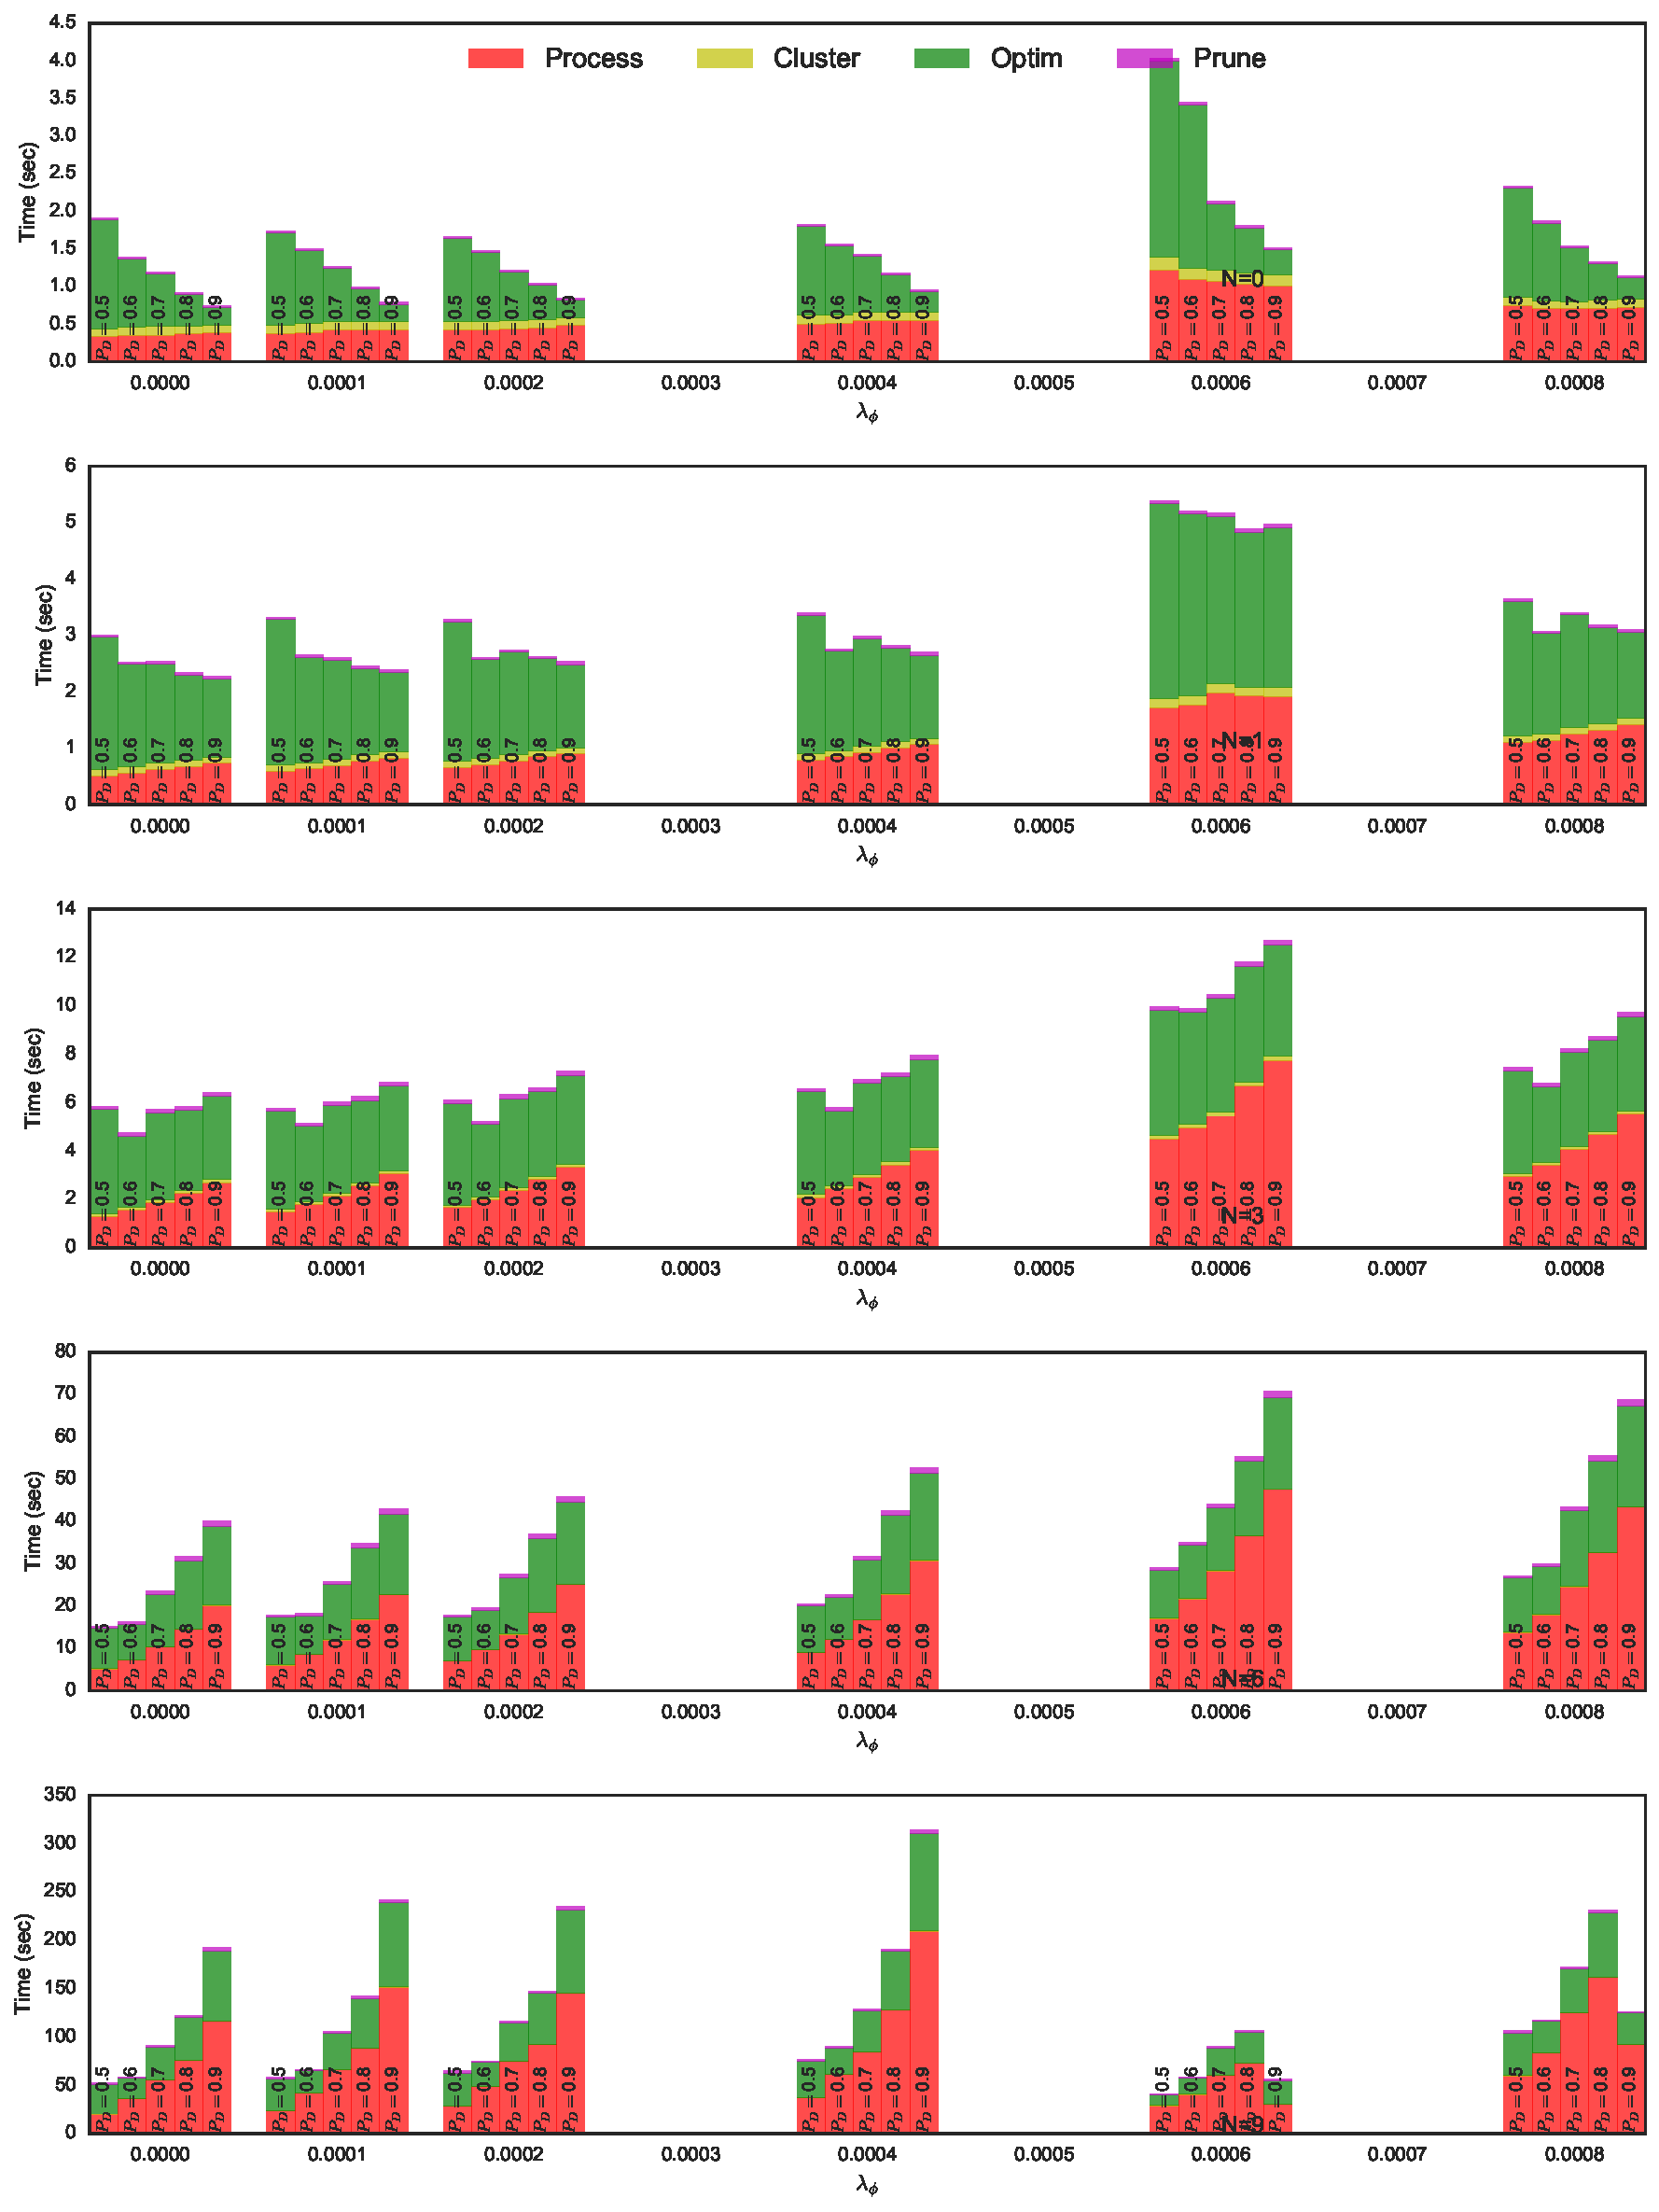
\includegraphics[width=\textwidth]{dynamic_agents_partial_cooporation_cropped-GLPK_runtimeLog}
	\caption{Scenario 2 - Run time log, GLPK solver}
	\label{fig:runtimelog_scenario2-GLPK}
\end{figure}\begin{figure}[H]
	\centering
	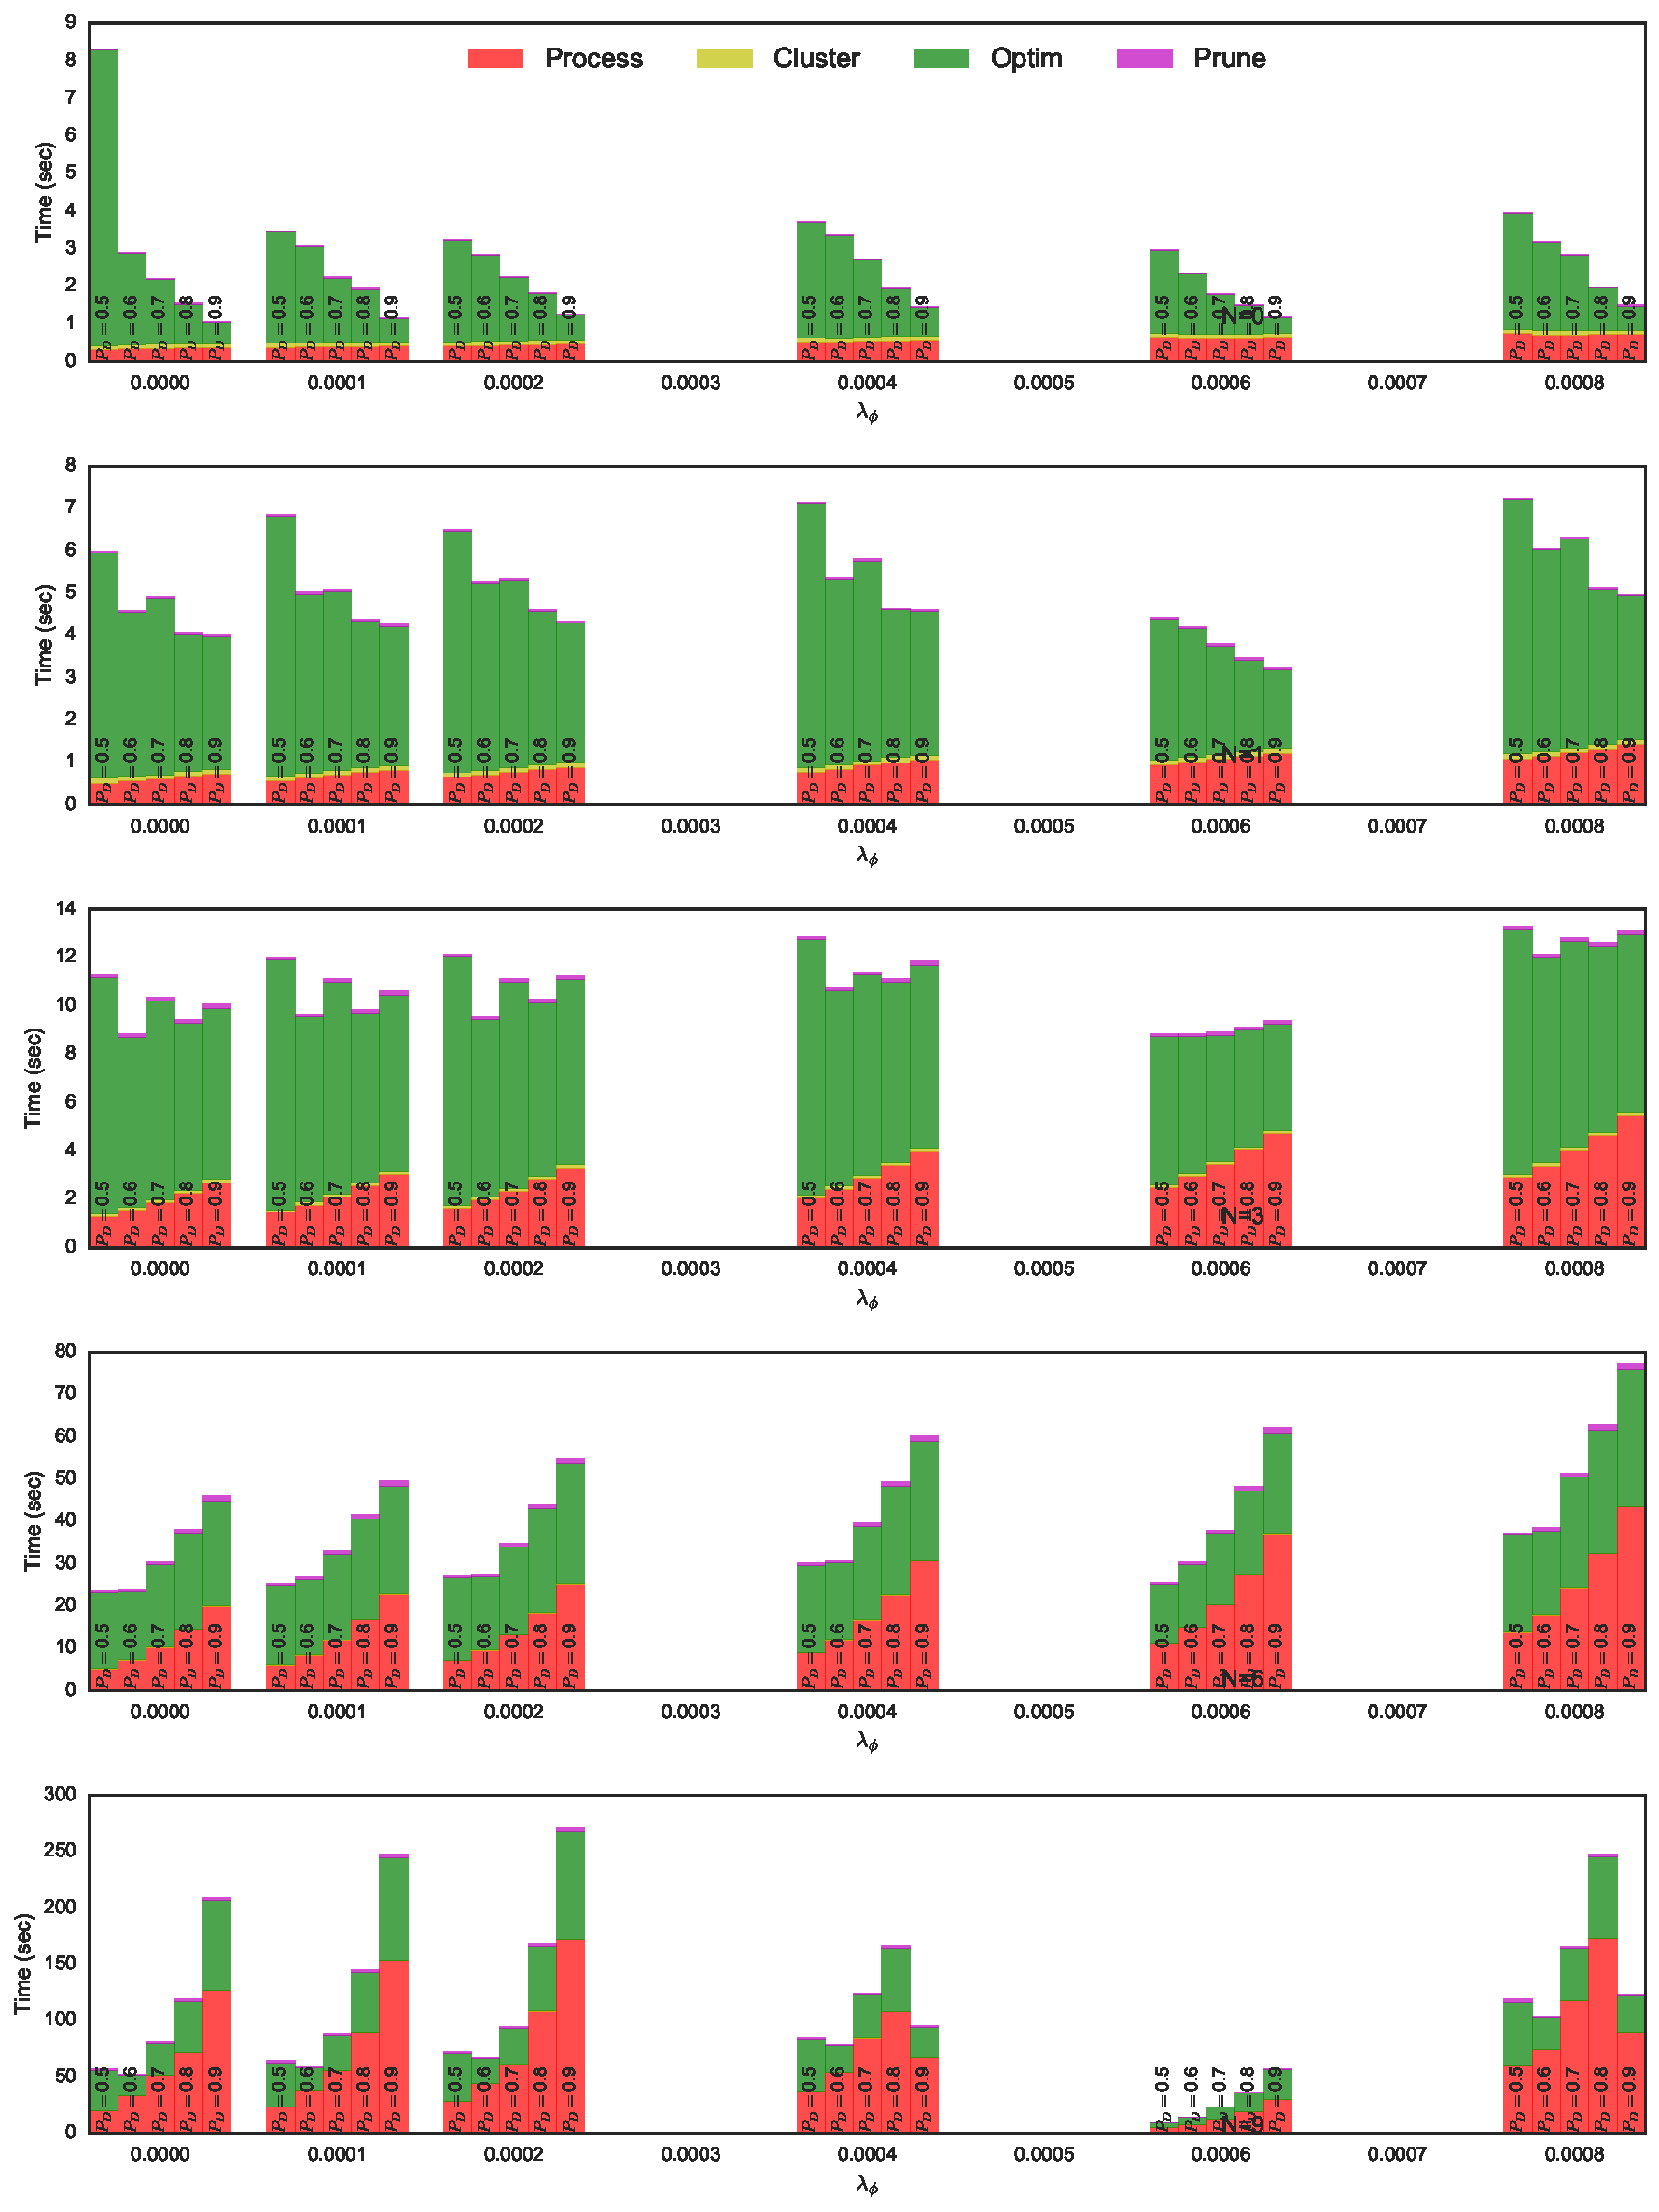
\includegraphics[width=\textwidth]{dynamic_agents_partial_cooporation_cropped-GUROBI_runtimeLog}
	\caption{Scenario 2 - Run time log, GUROBI solver}
	\label{fig:runtimelog_scenario2-GUROBI}
\end{figure}


\begin{figure}[H]
	\centering
	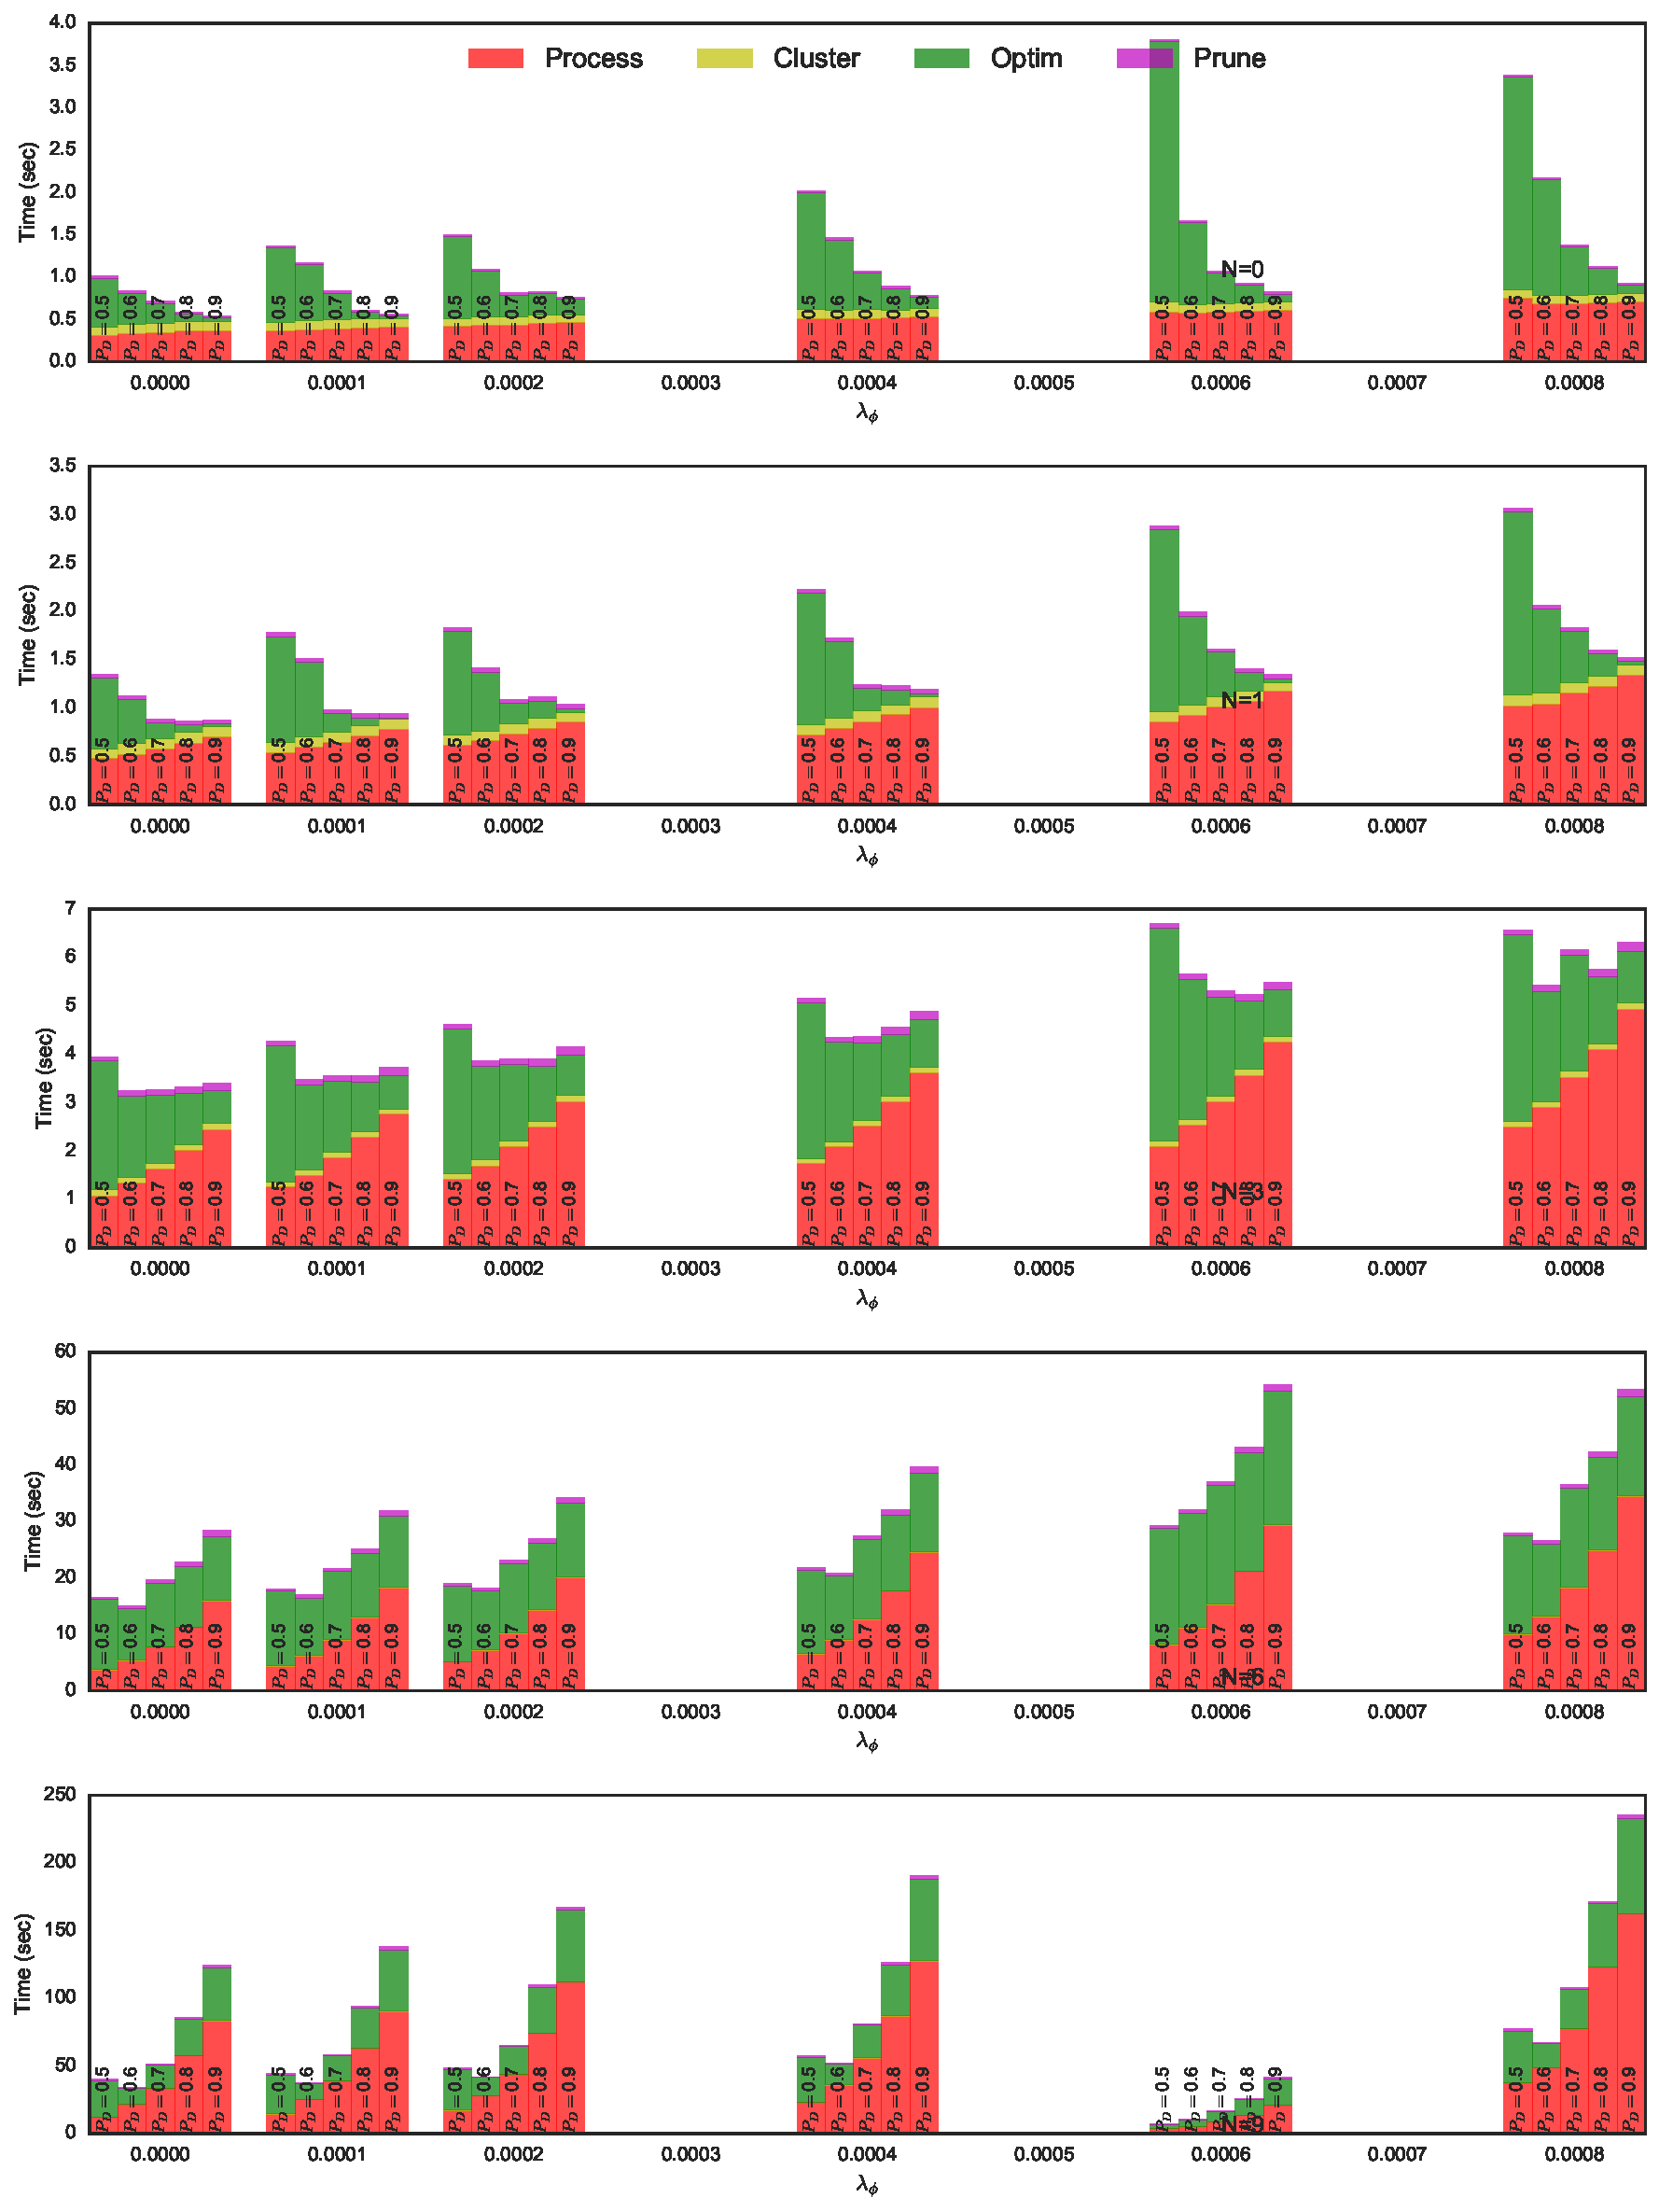
\includegraphics[width=\textwidth]{dynamic_and_static_agents_large_space_cropped-CBC_runtimeLog}
	\caption{Scenario3 - Run time log, CBC solver}
	\label{fig:runtimelog_scenario3-CBC}
\end{figure}
\begin{figure}[H]
	\centering
	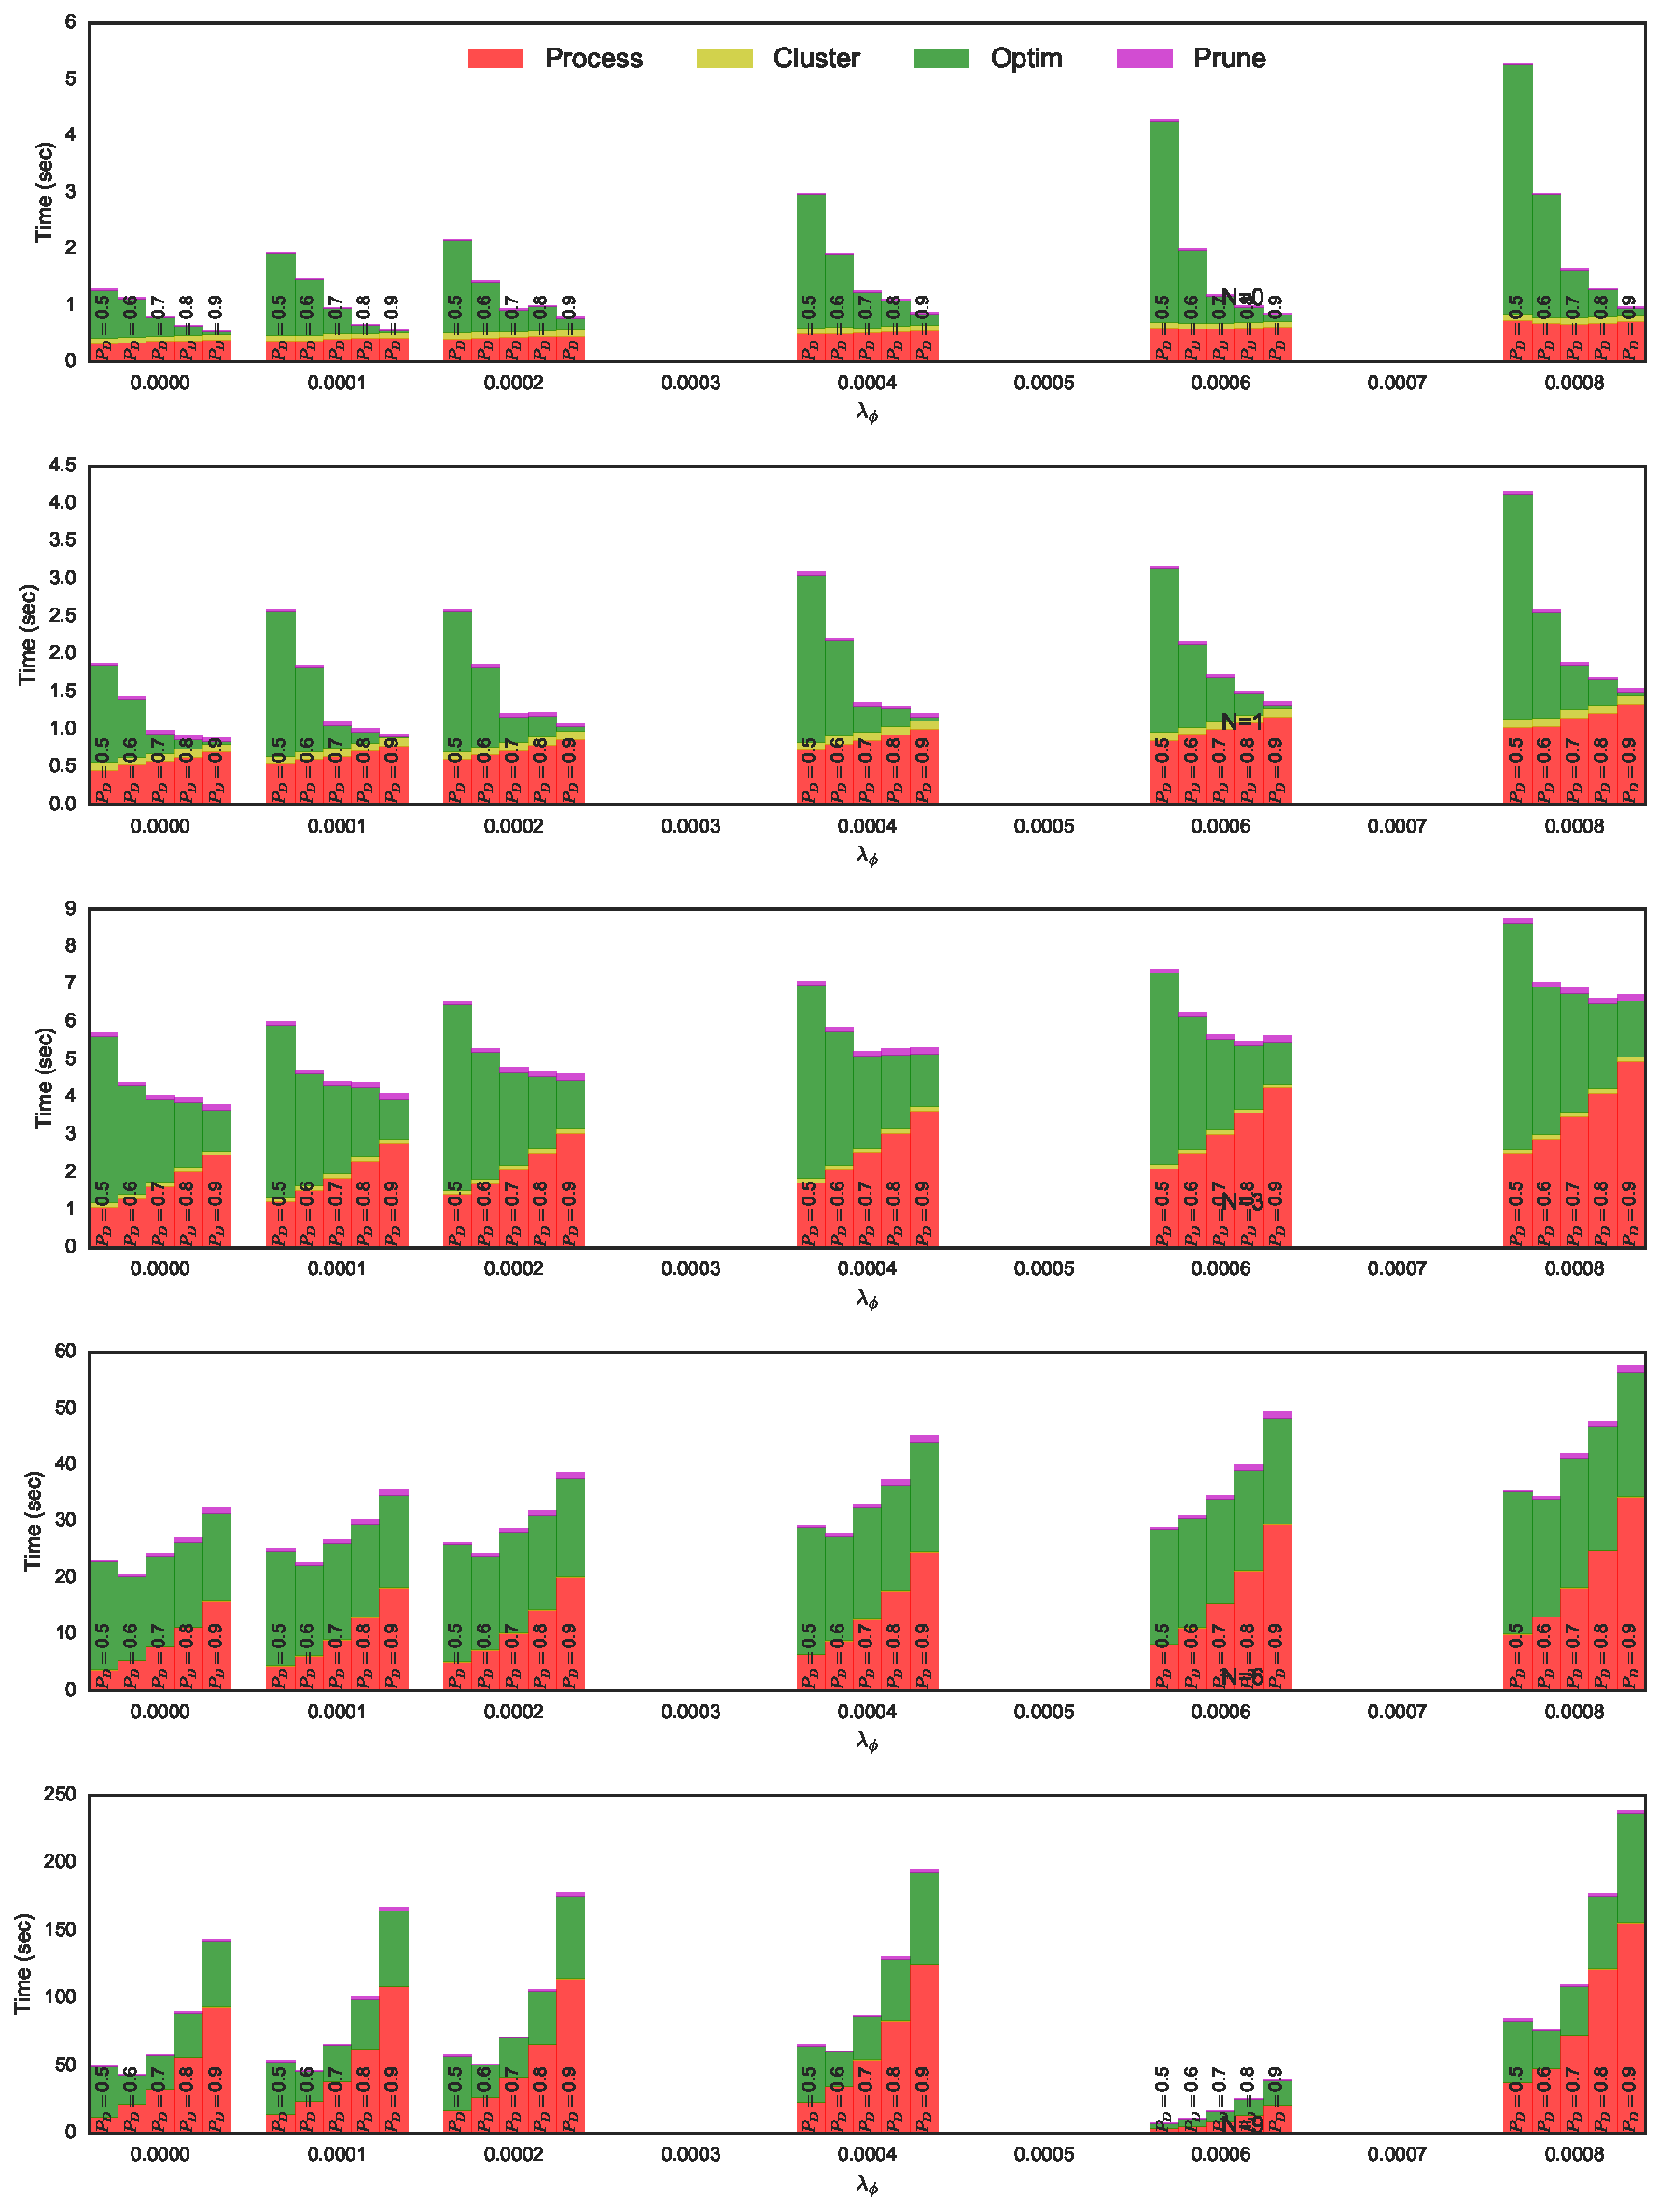
\includegraphics[width=\textwidth]{dynamic_and_static_agents_large_space_cropped-CPLEX_runtimeLog}
	\caption{Scenario3 - Run time log, CPLEX solver}
	\label{fig:runtimelog_scenario3-CPLEX}
\end{figure}
\begin{figure}[H]
	\centering
	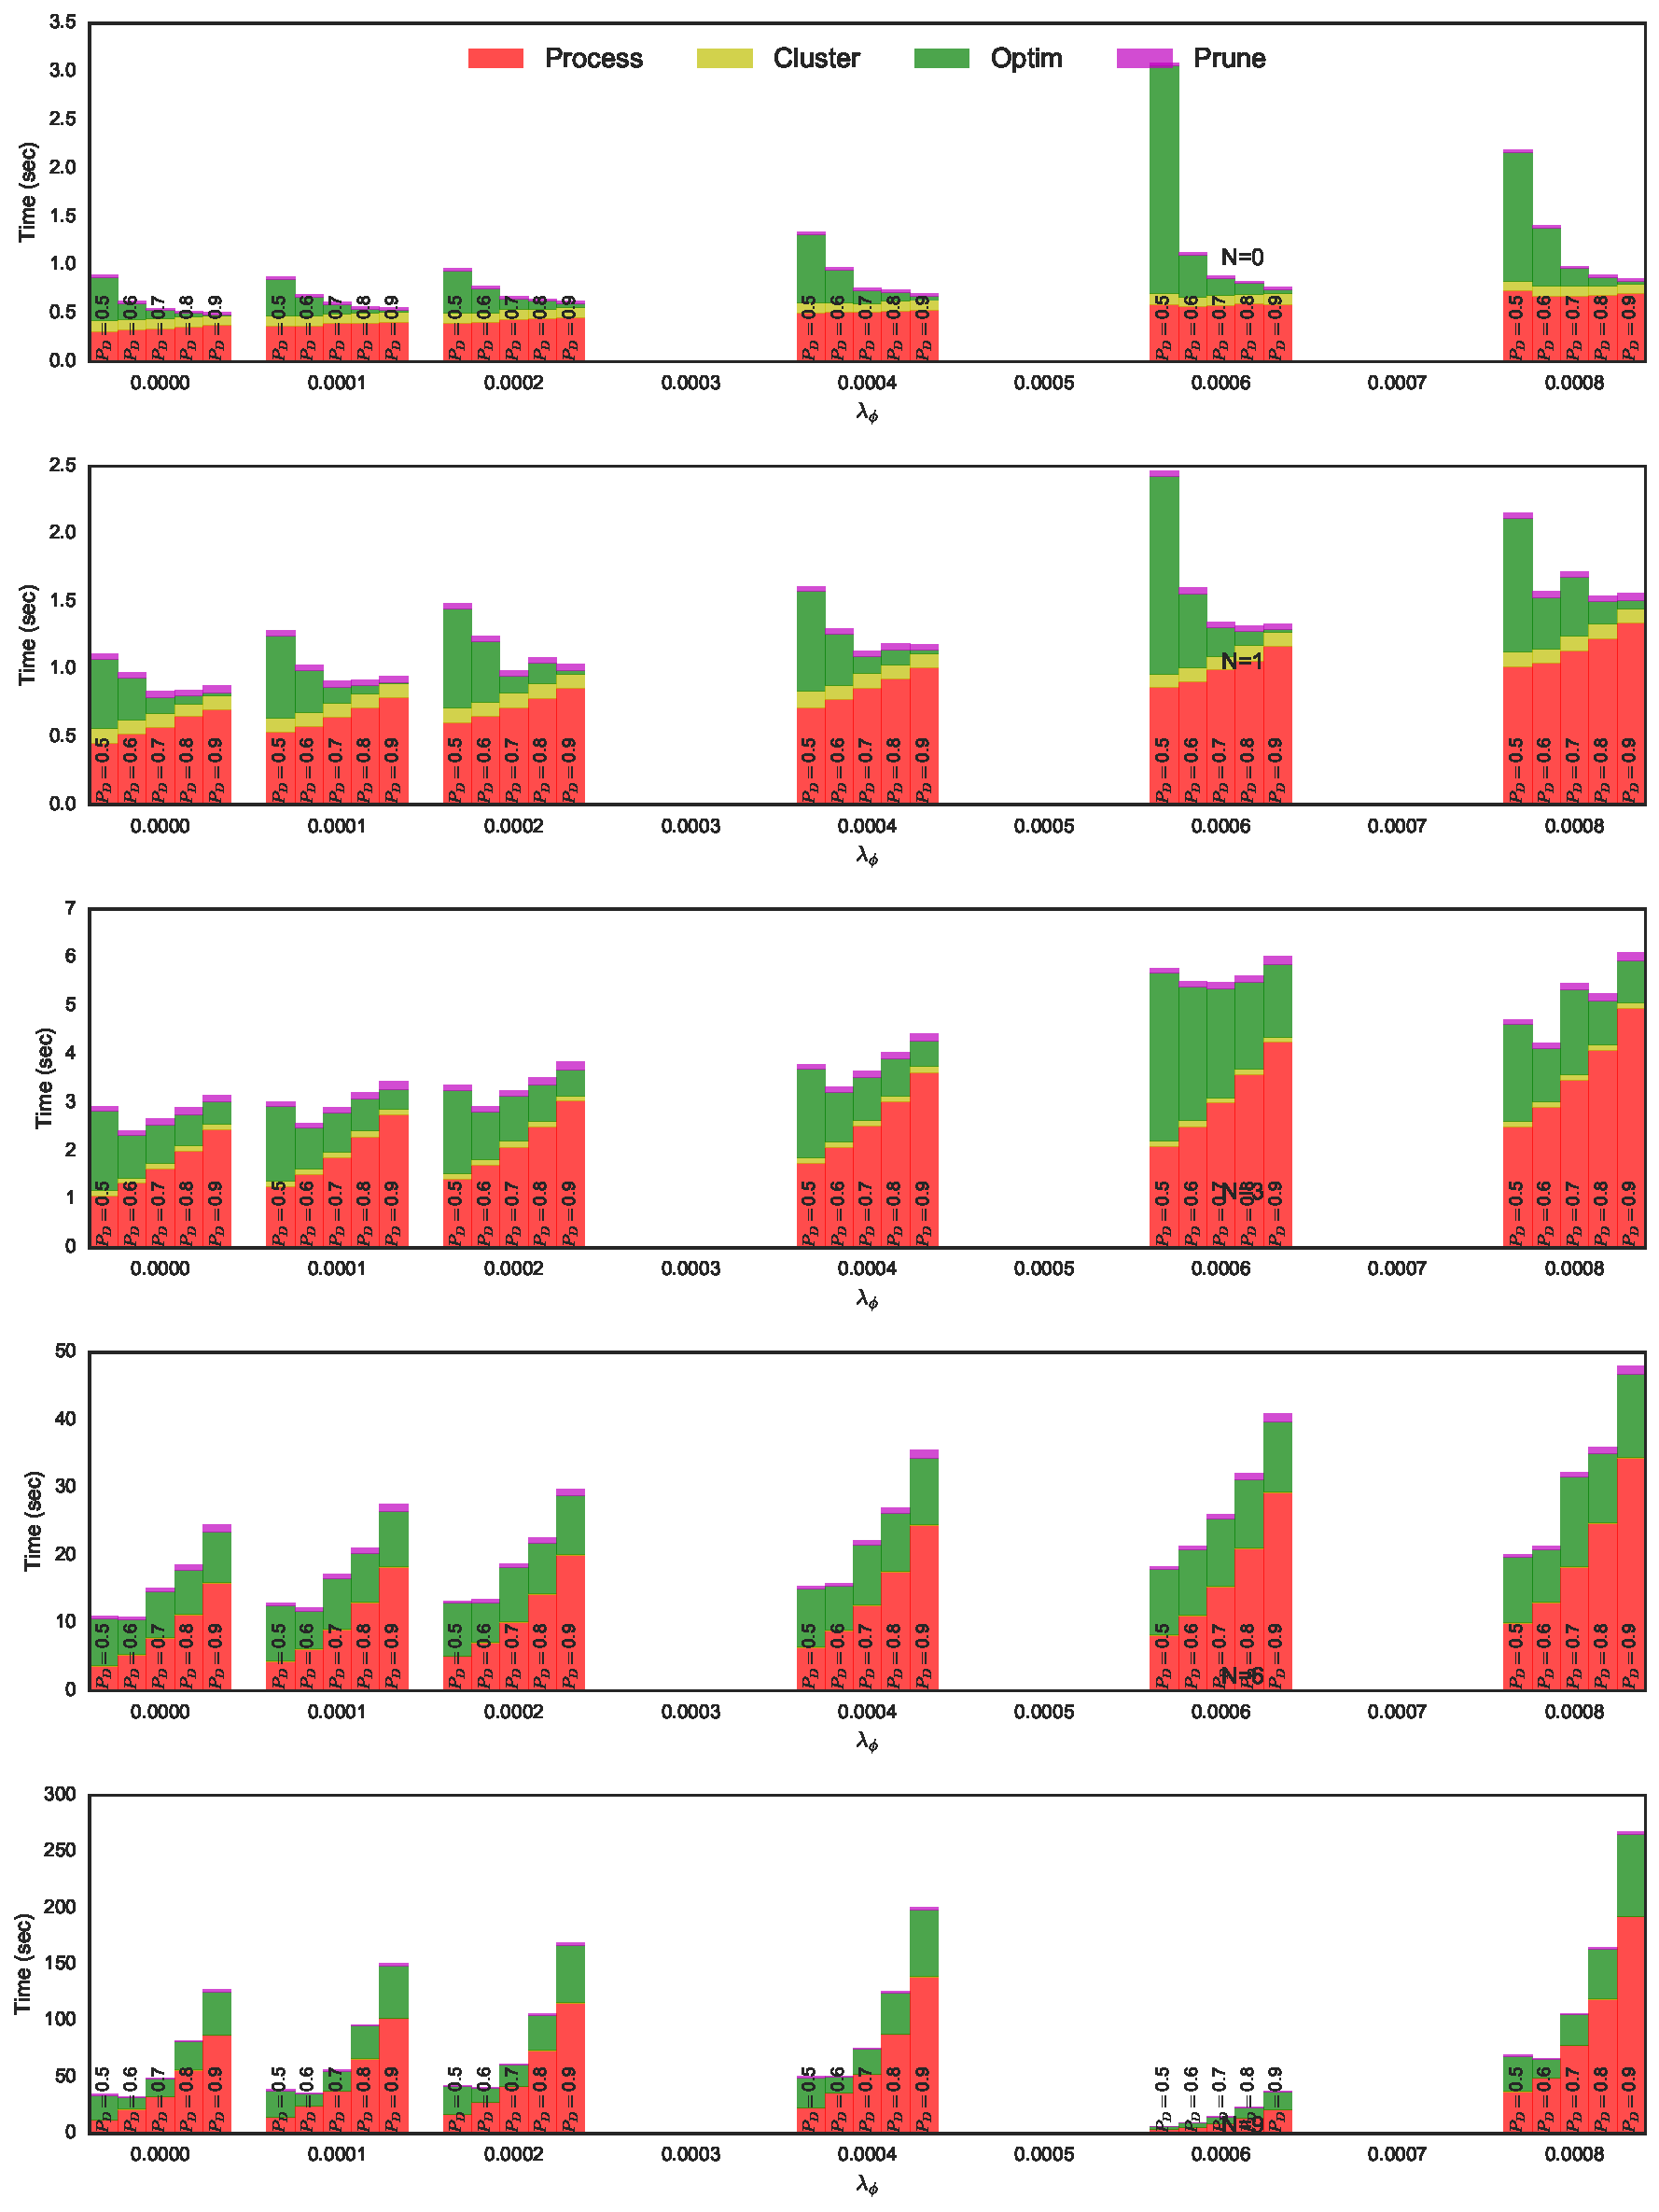
\includegraphics[width=\textwidth]{dynamic_and_static_agents_large_space_cropped-GLPK_runtimeLog}
	\caption{Scenario3 - Run time log, GLPK solver}
	\label{fig:runtimelog_scenario3-GLPK}
\end{figure}
\begin{figure}[H]
	\centering
	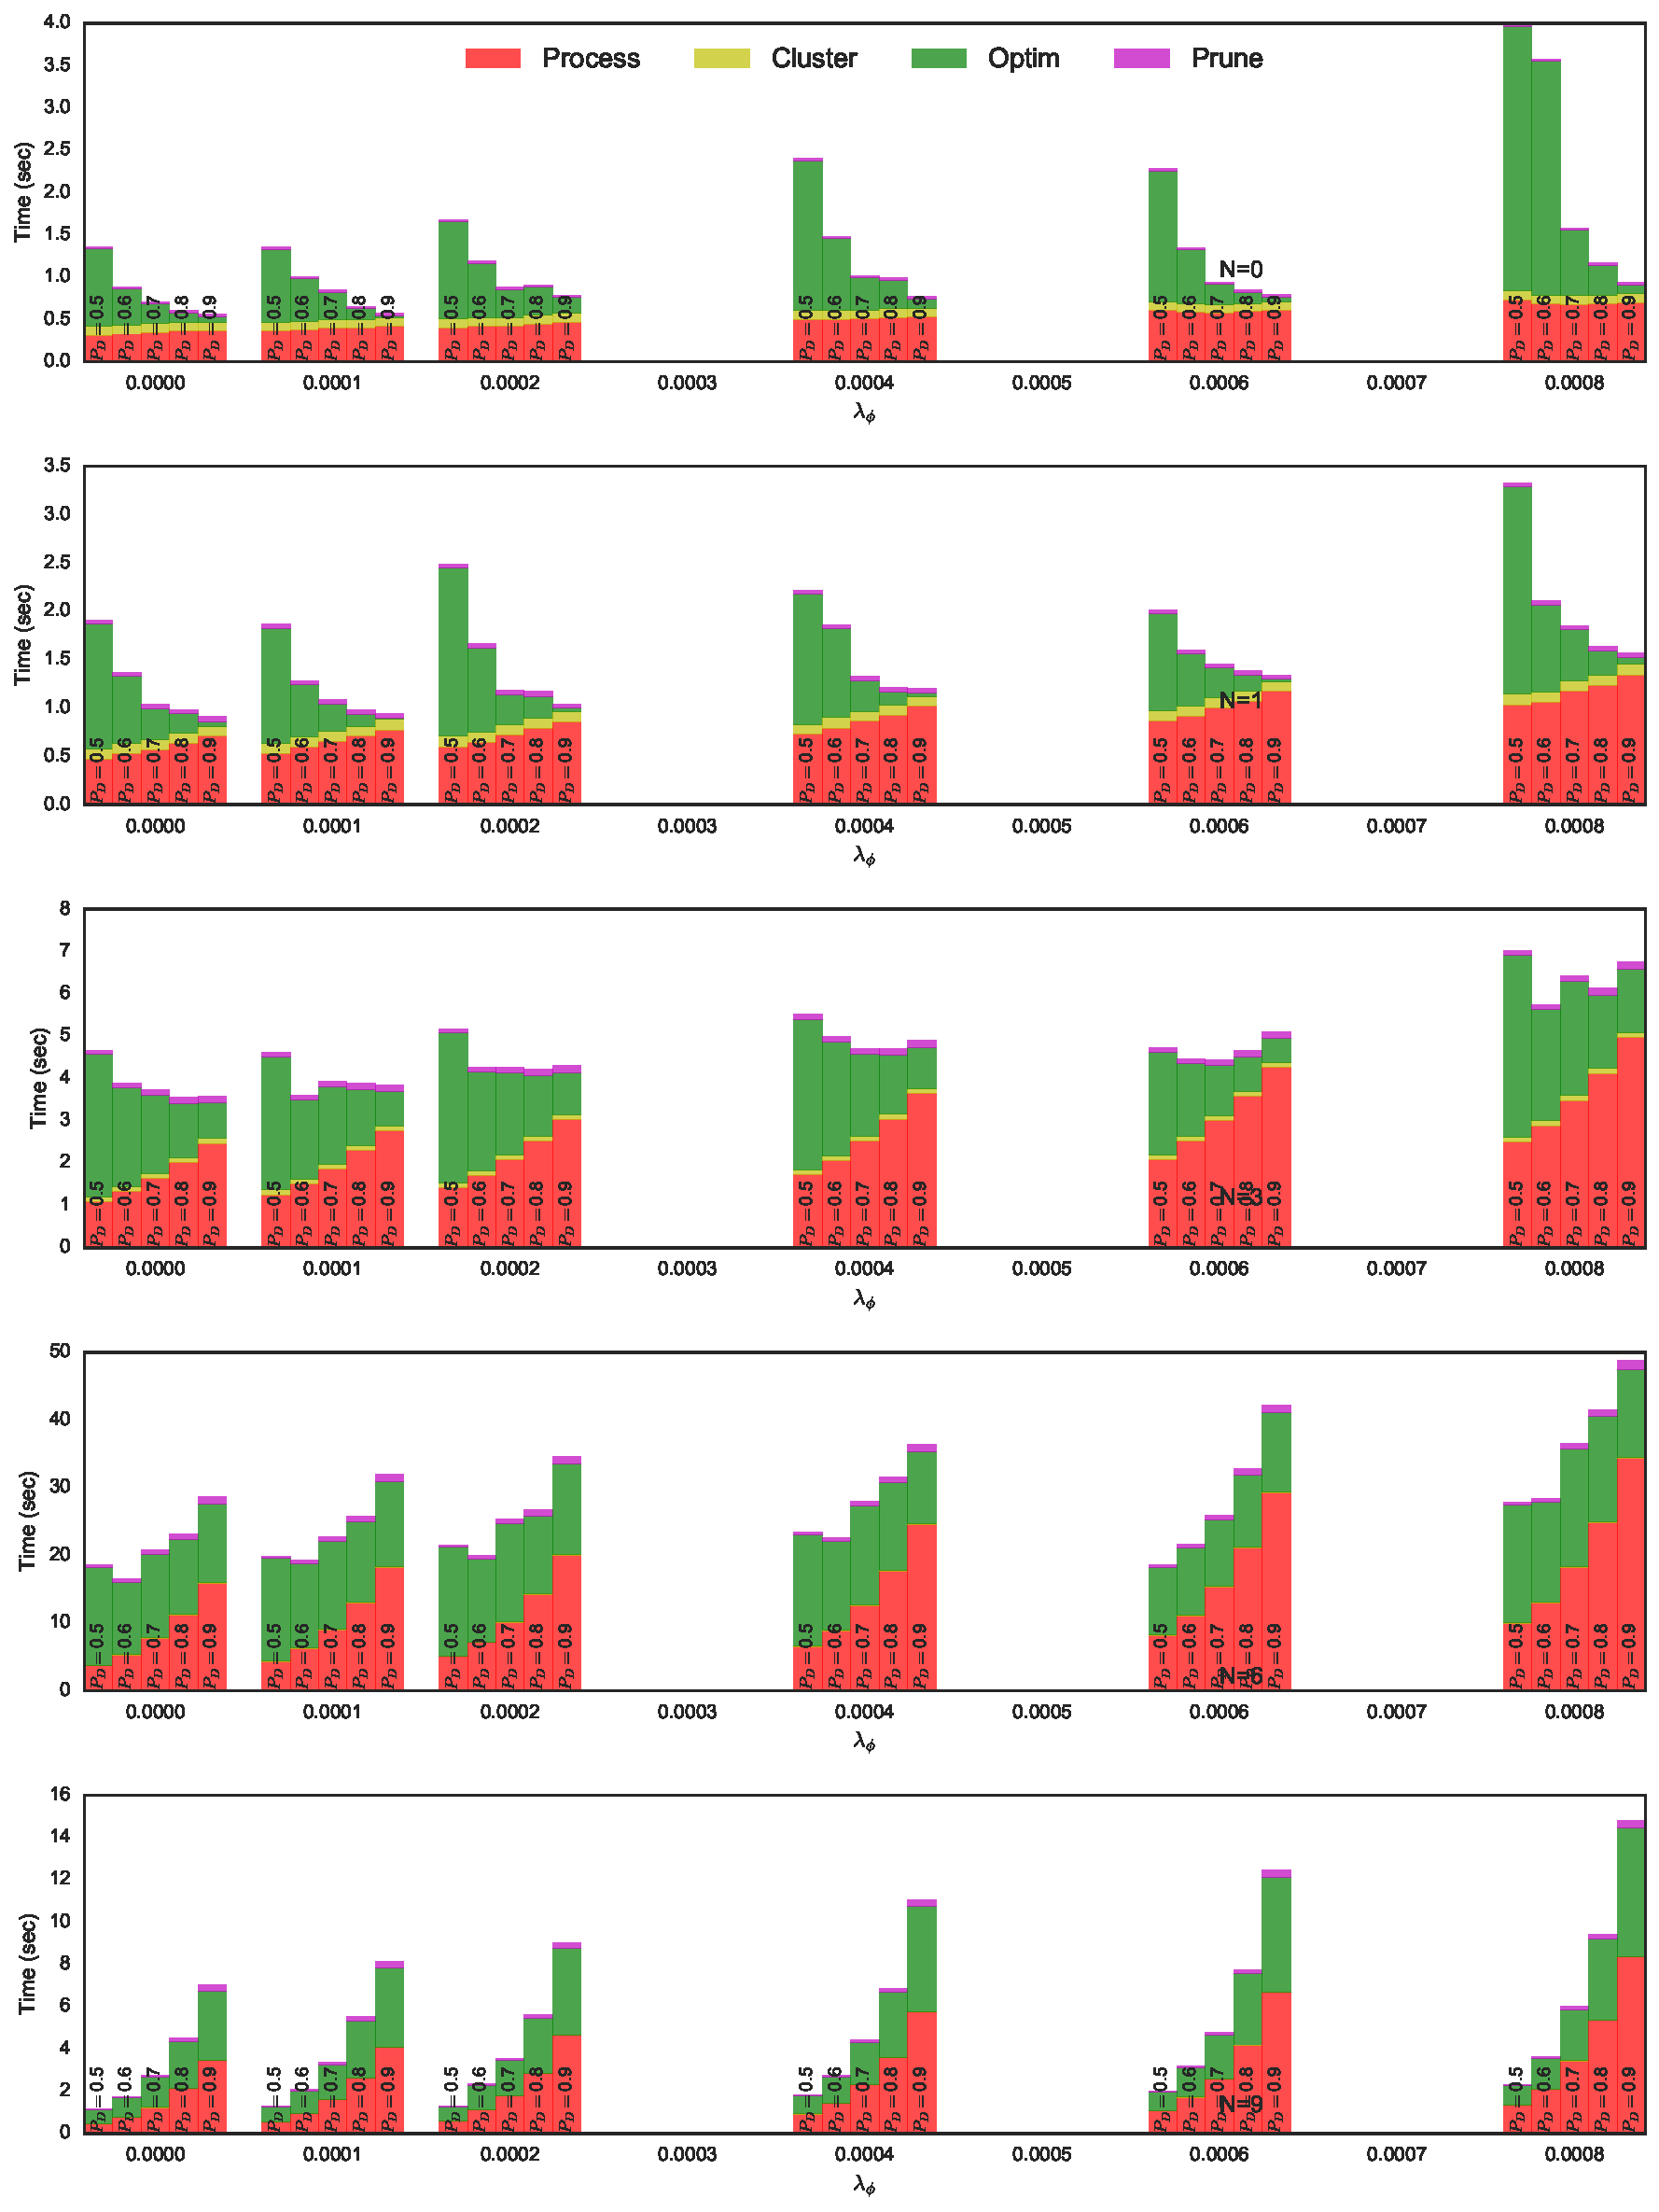
\includegraphics[width=\textwidth]{dynamic_and_static_agents_large_space_cropped-GUROBI_runtimeLog}
	\caption{Scenario3 - Run time log, GUROBI solver}
	\label{fig:runtimelog_scenario3-GUROBI}
\end{figure}


\begin{figure}[H]
	\centering
	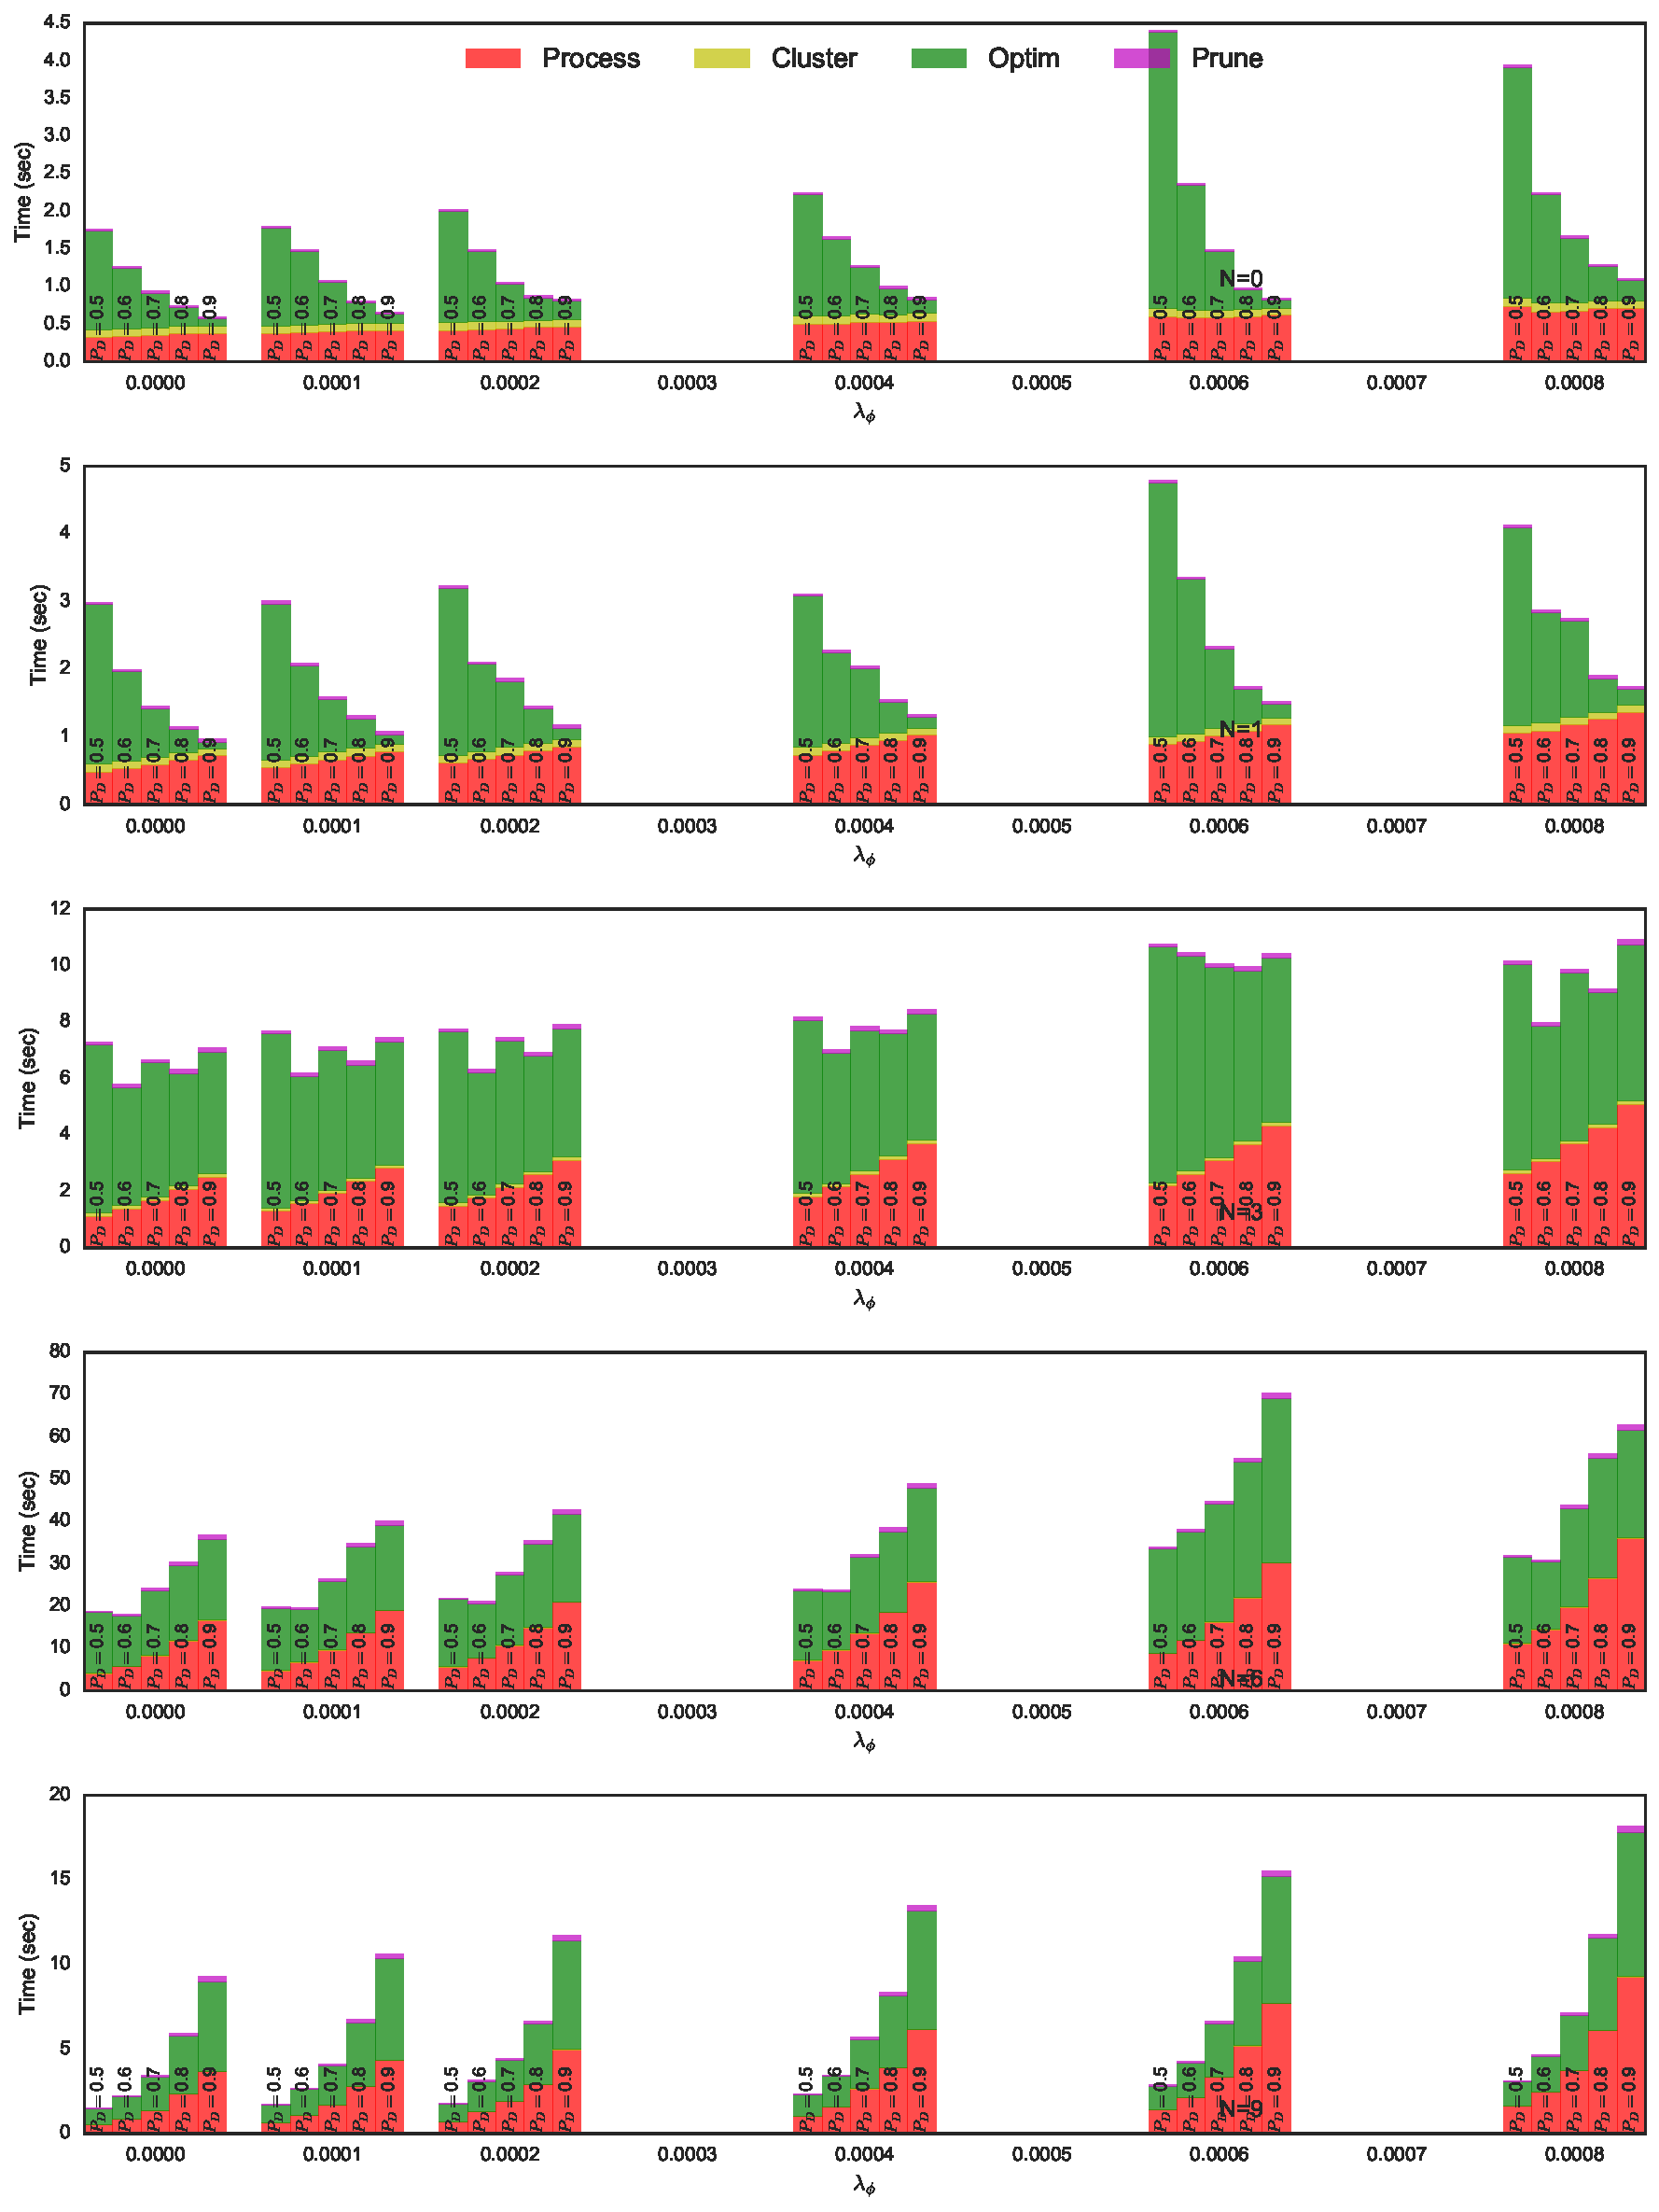
\includegraphics[width=\textwidth]{dynamic_and_static_agents_narrow_space_cropped-CBC_runtimeLog}
	\caption{Scenario 4 - Run time log, CBC solver}
	\label{fig:runtimelog_scenario4-CBC}
\end{figure}
\begin{figure}[H]
	\centering
	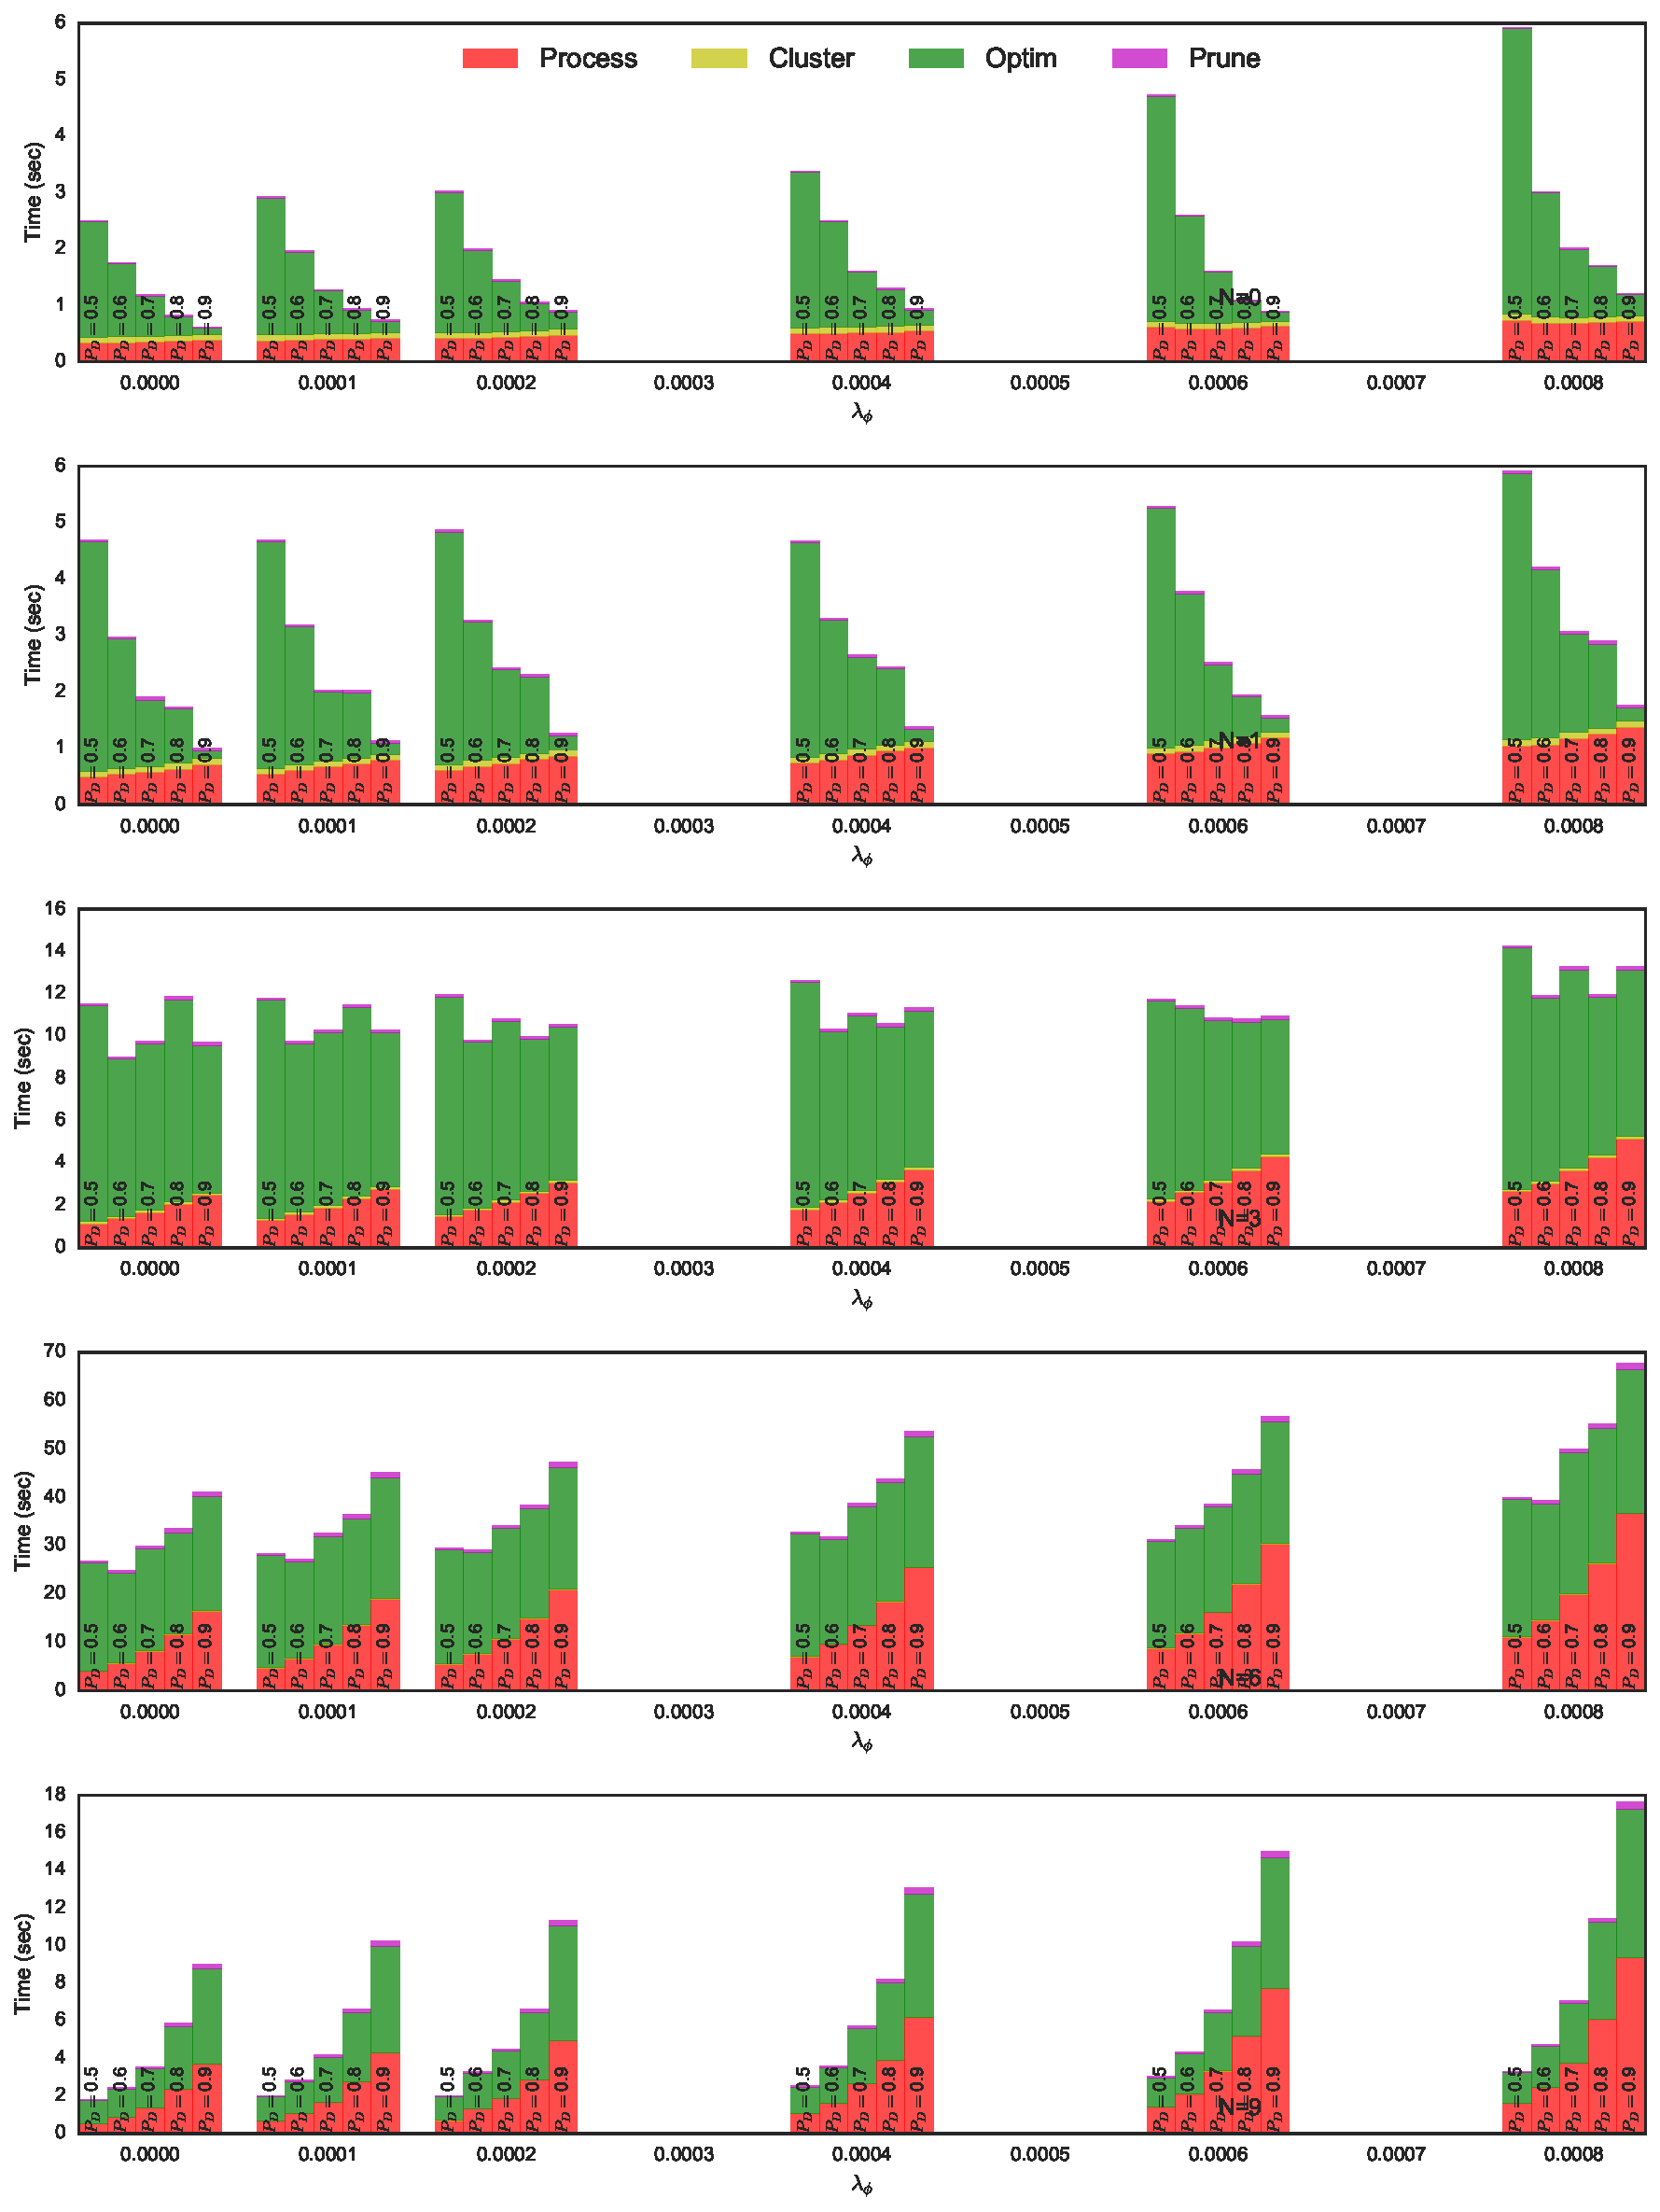
\includegraphics[width=\textwidth]{dynamic_and_static_agents_narrow_space_cropped-CPLEX_runtimeLog}
	\caption{Scenario 4 - Run time log, CPLEX solver}
	\label{fig:runtimelog_scenario4-CPLEX}
\end{figure}
\begin{figure}[H]
	\centering
	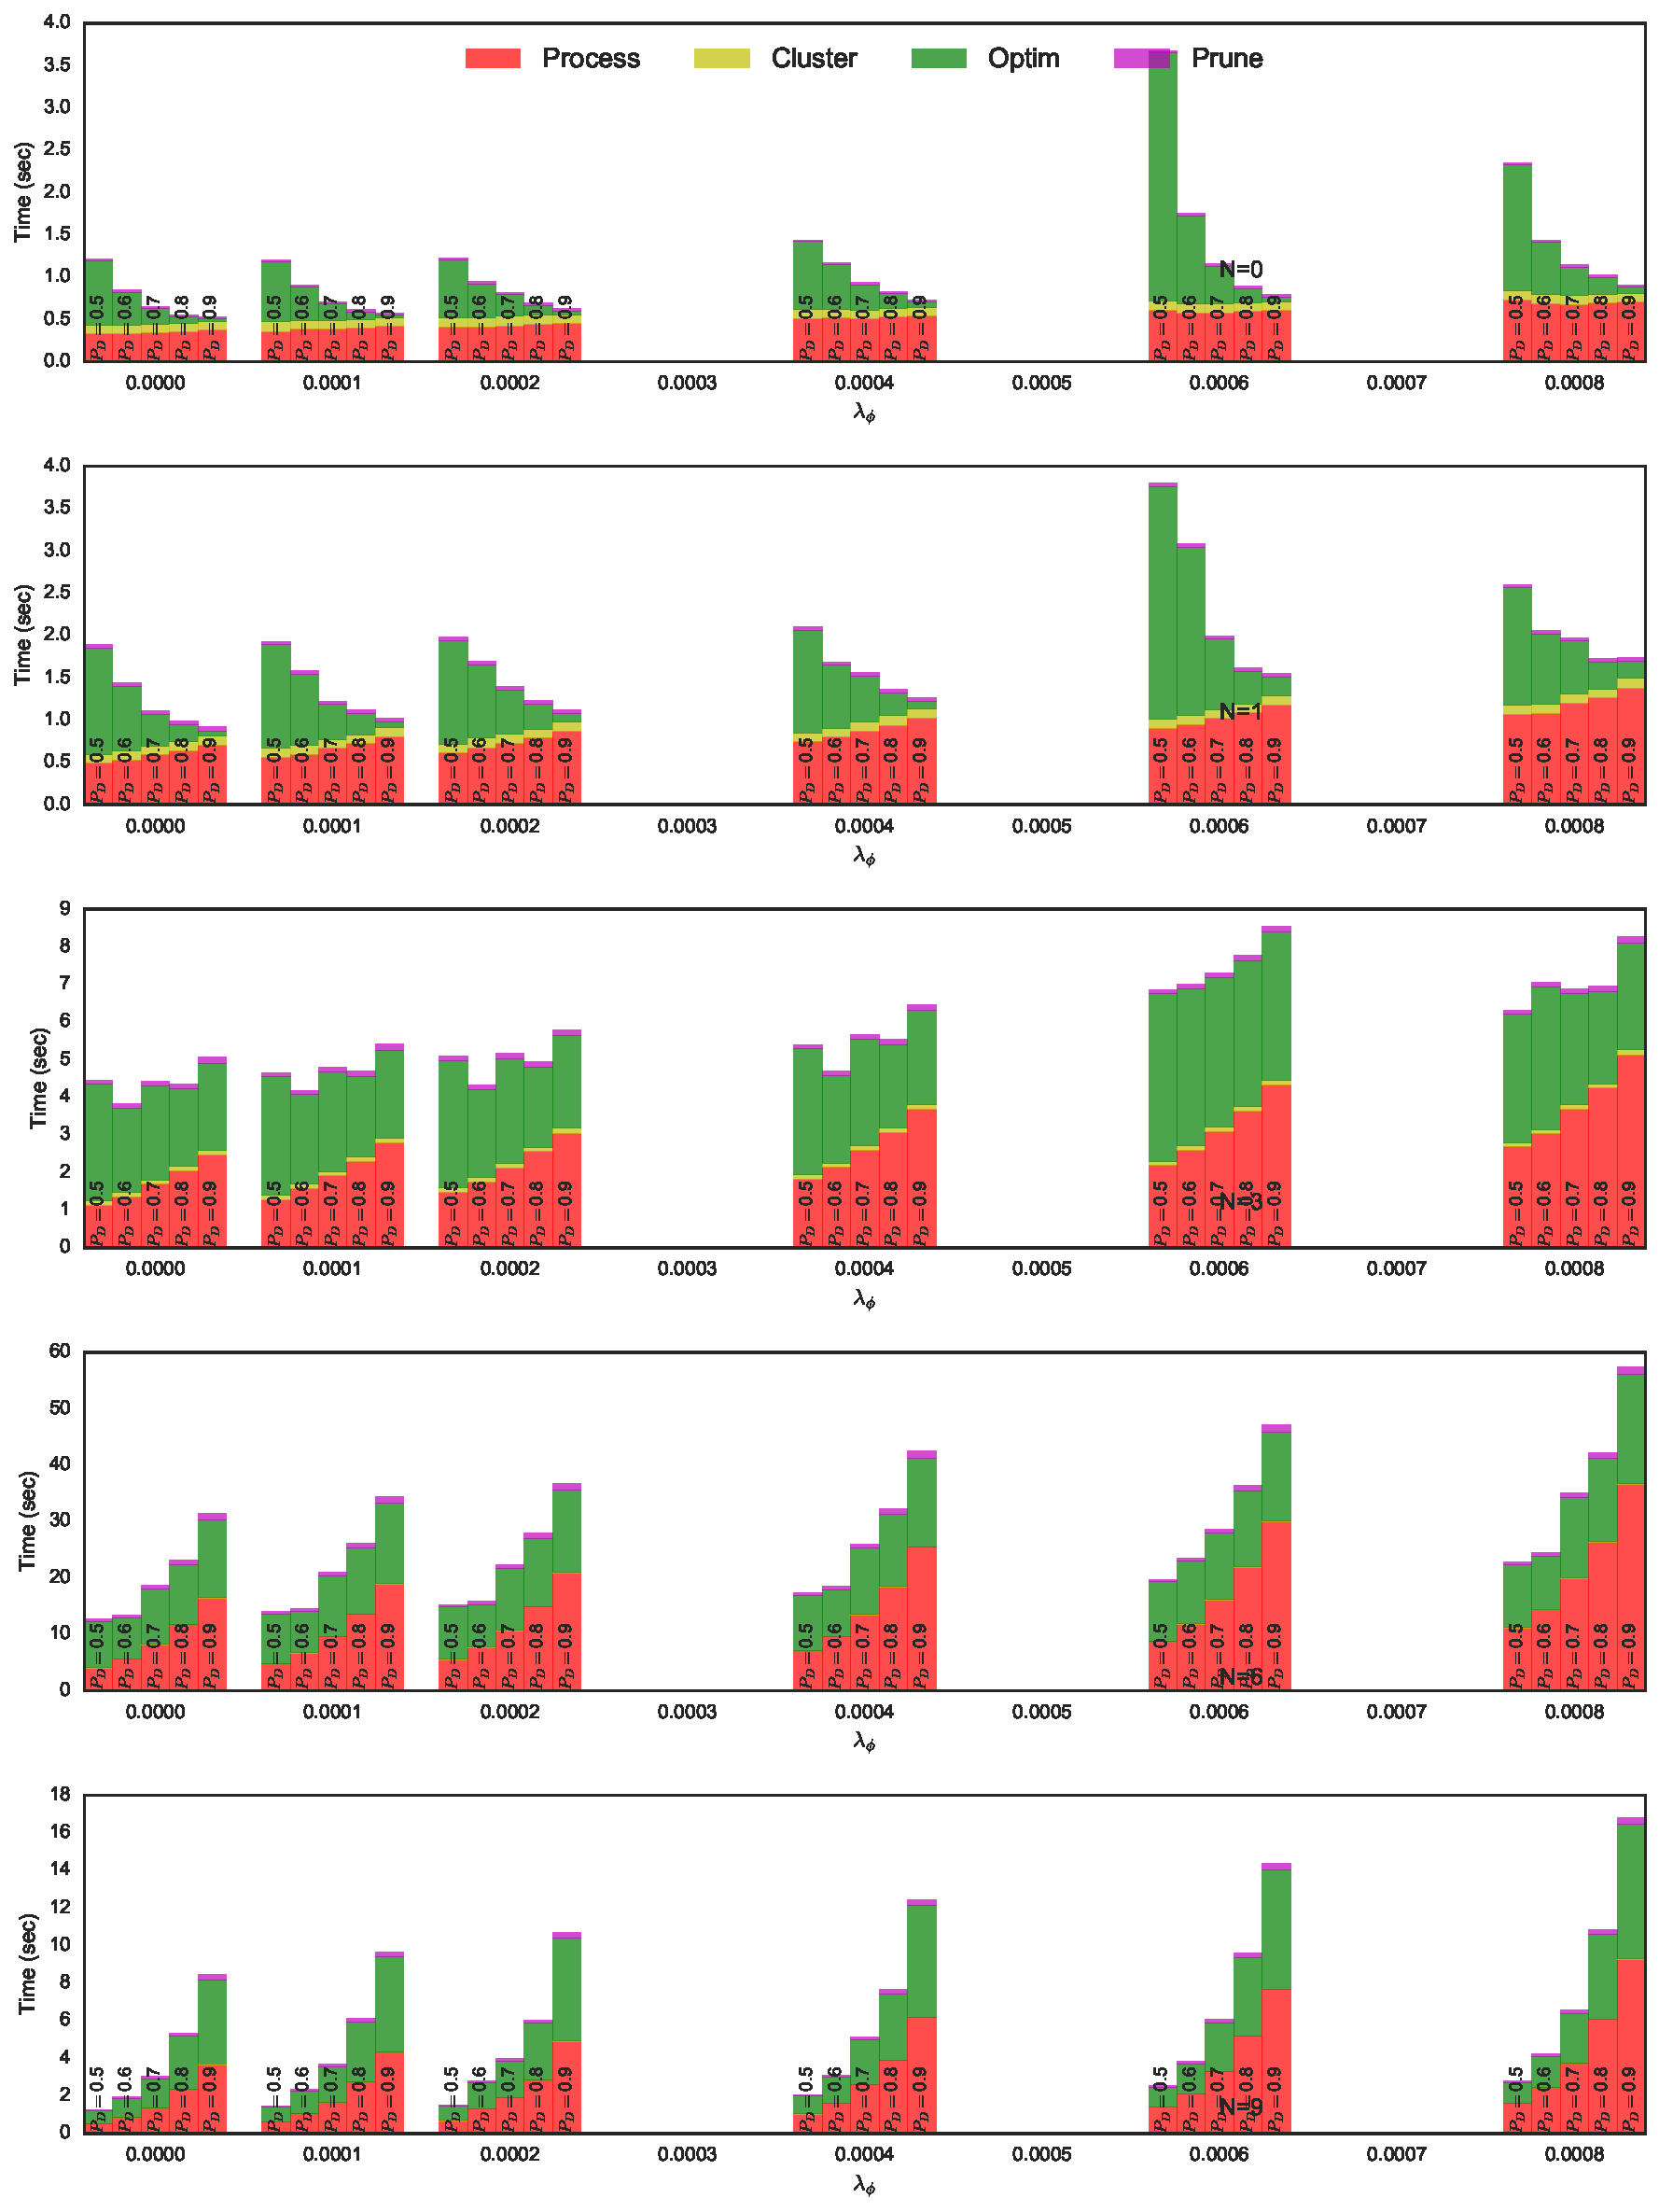
\includegraphics[width=\textwidth]{dynamic_and_static_agents_narrow_space_cropped-GLPK_runtimeLog}
	\caption{Scenario 4 - Run time log, GLPK solver}
	\label{fig:runtimelog_scenario4-GLPK}
\end{figure}
\begin{figure}[H]
	\centering
	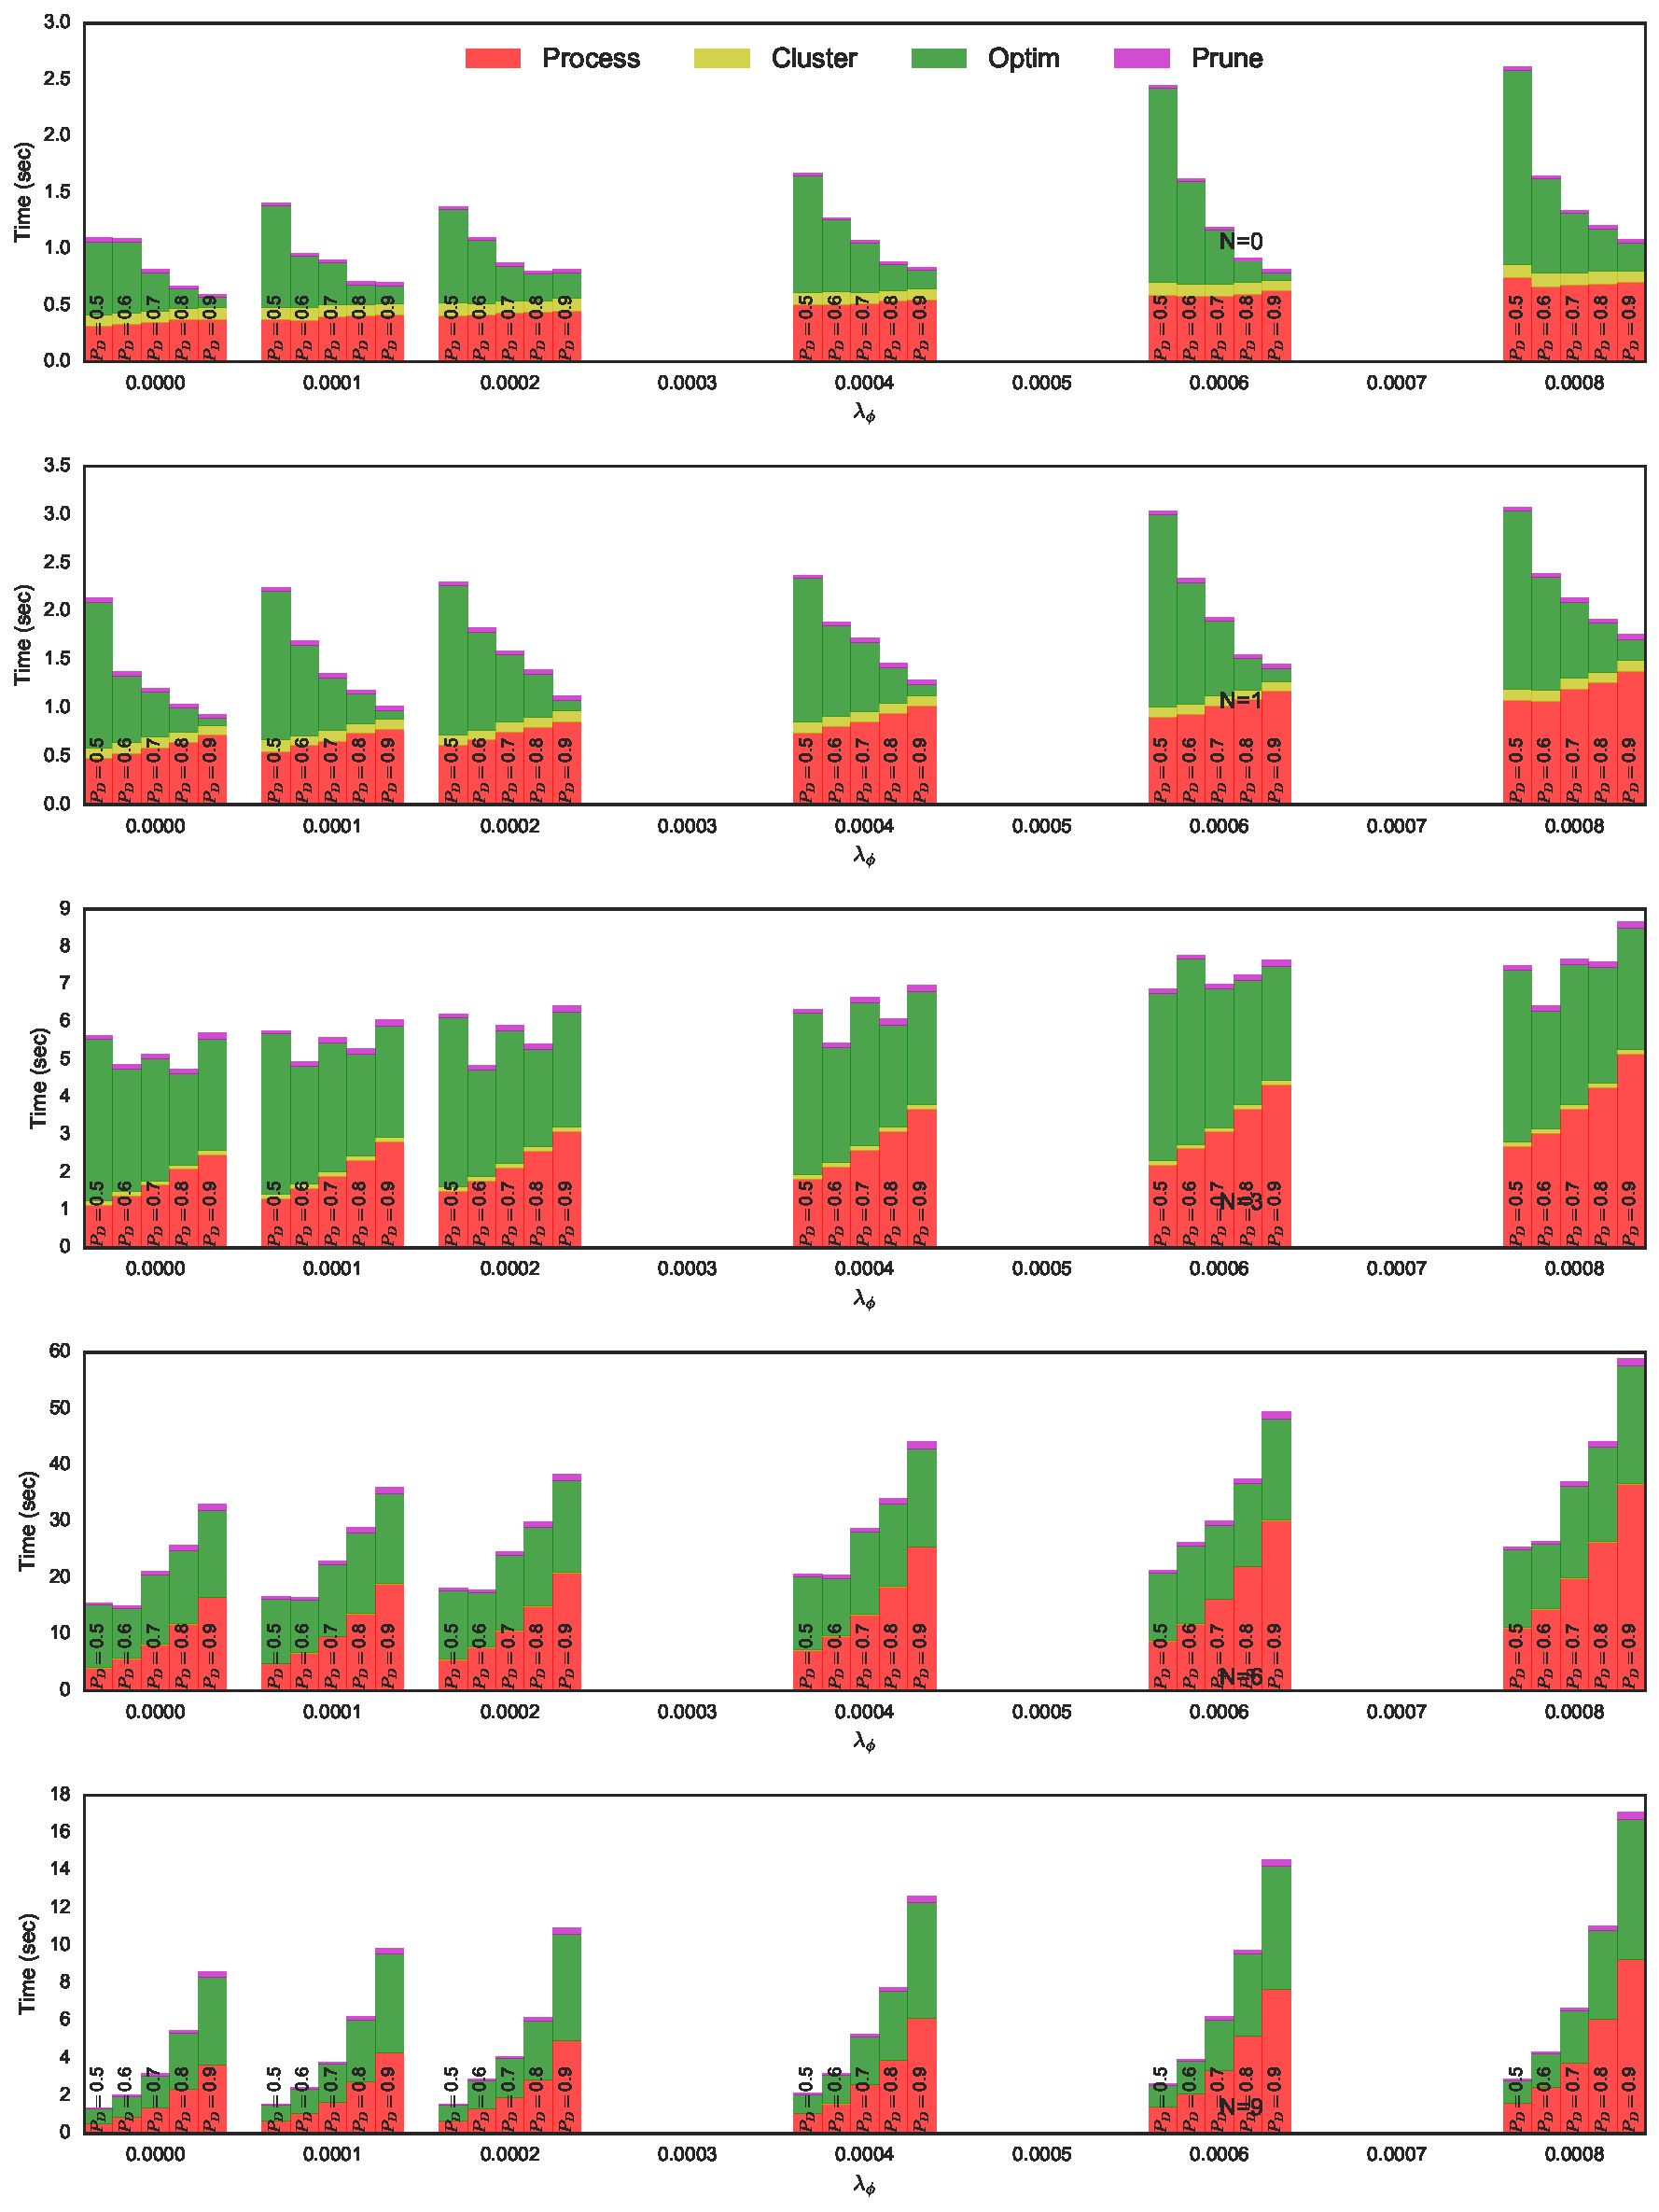
\includegraphics[width=\textwidth]{dynamic_and_static_agents_narrow_space_cropped-GUROBI_runtimeLog}
	\caption{Scenario 4 - Run time log, GUROBI solver}
	\label{fig:runtimelog_scenario4-GUROBI}
\end{figure}


\begin{figure}[H]
	\centering
	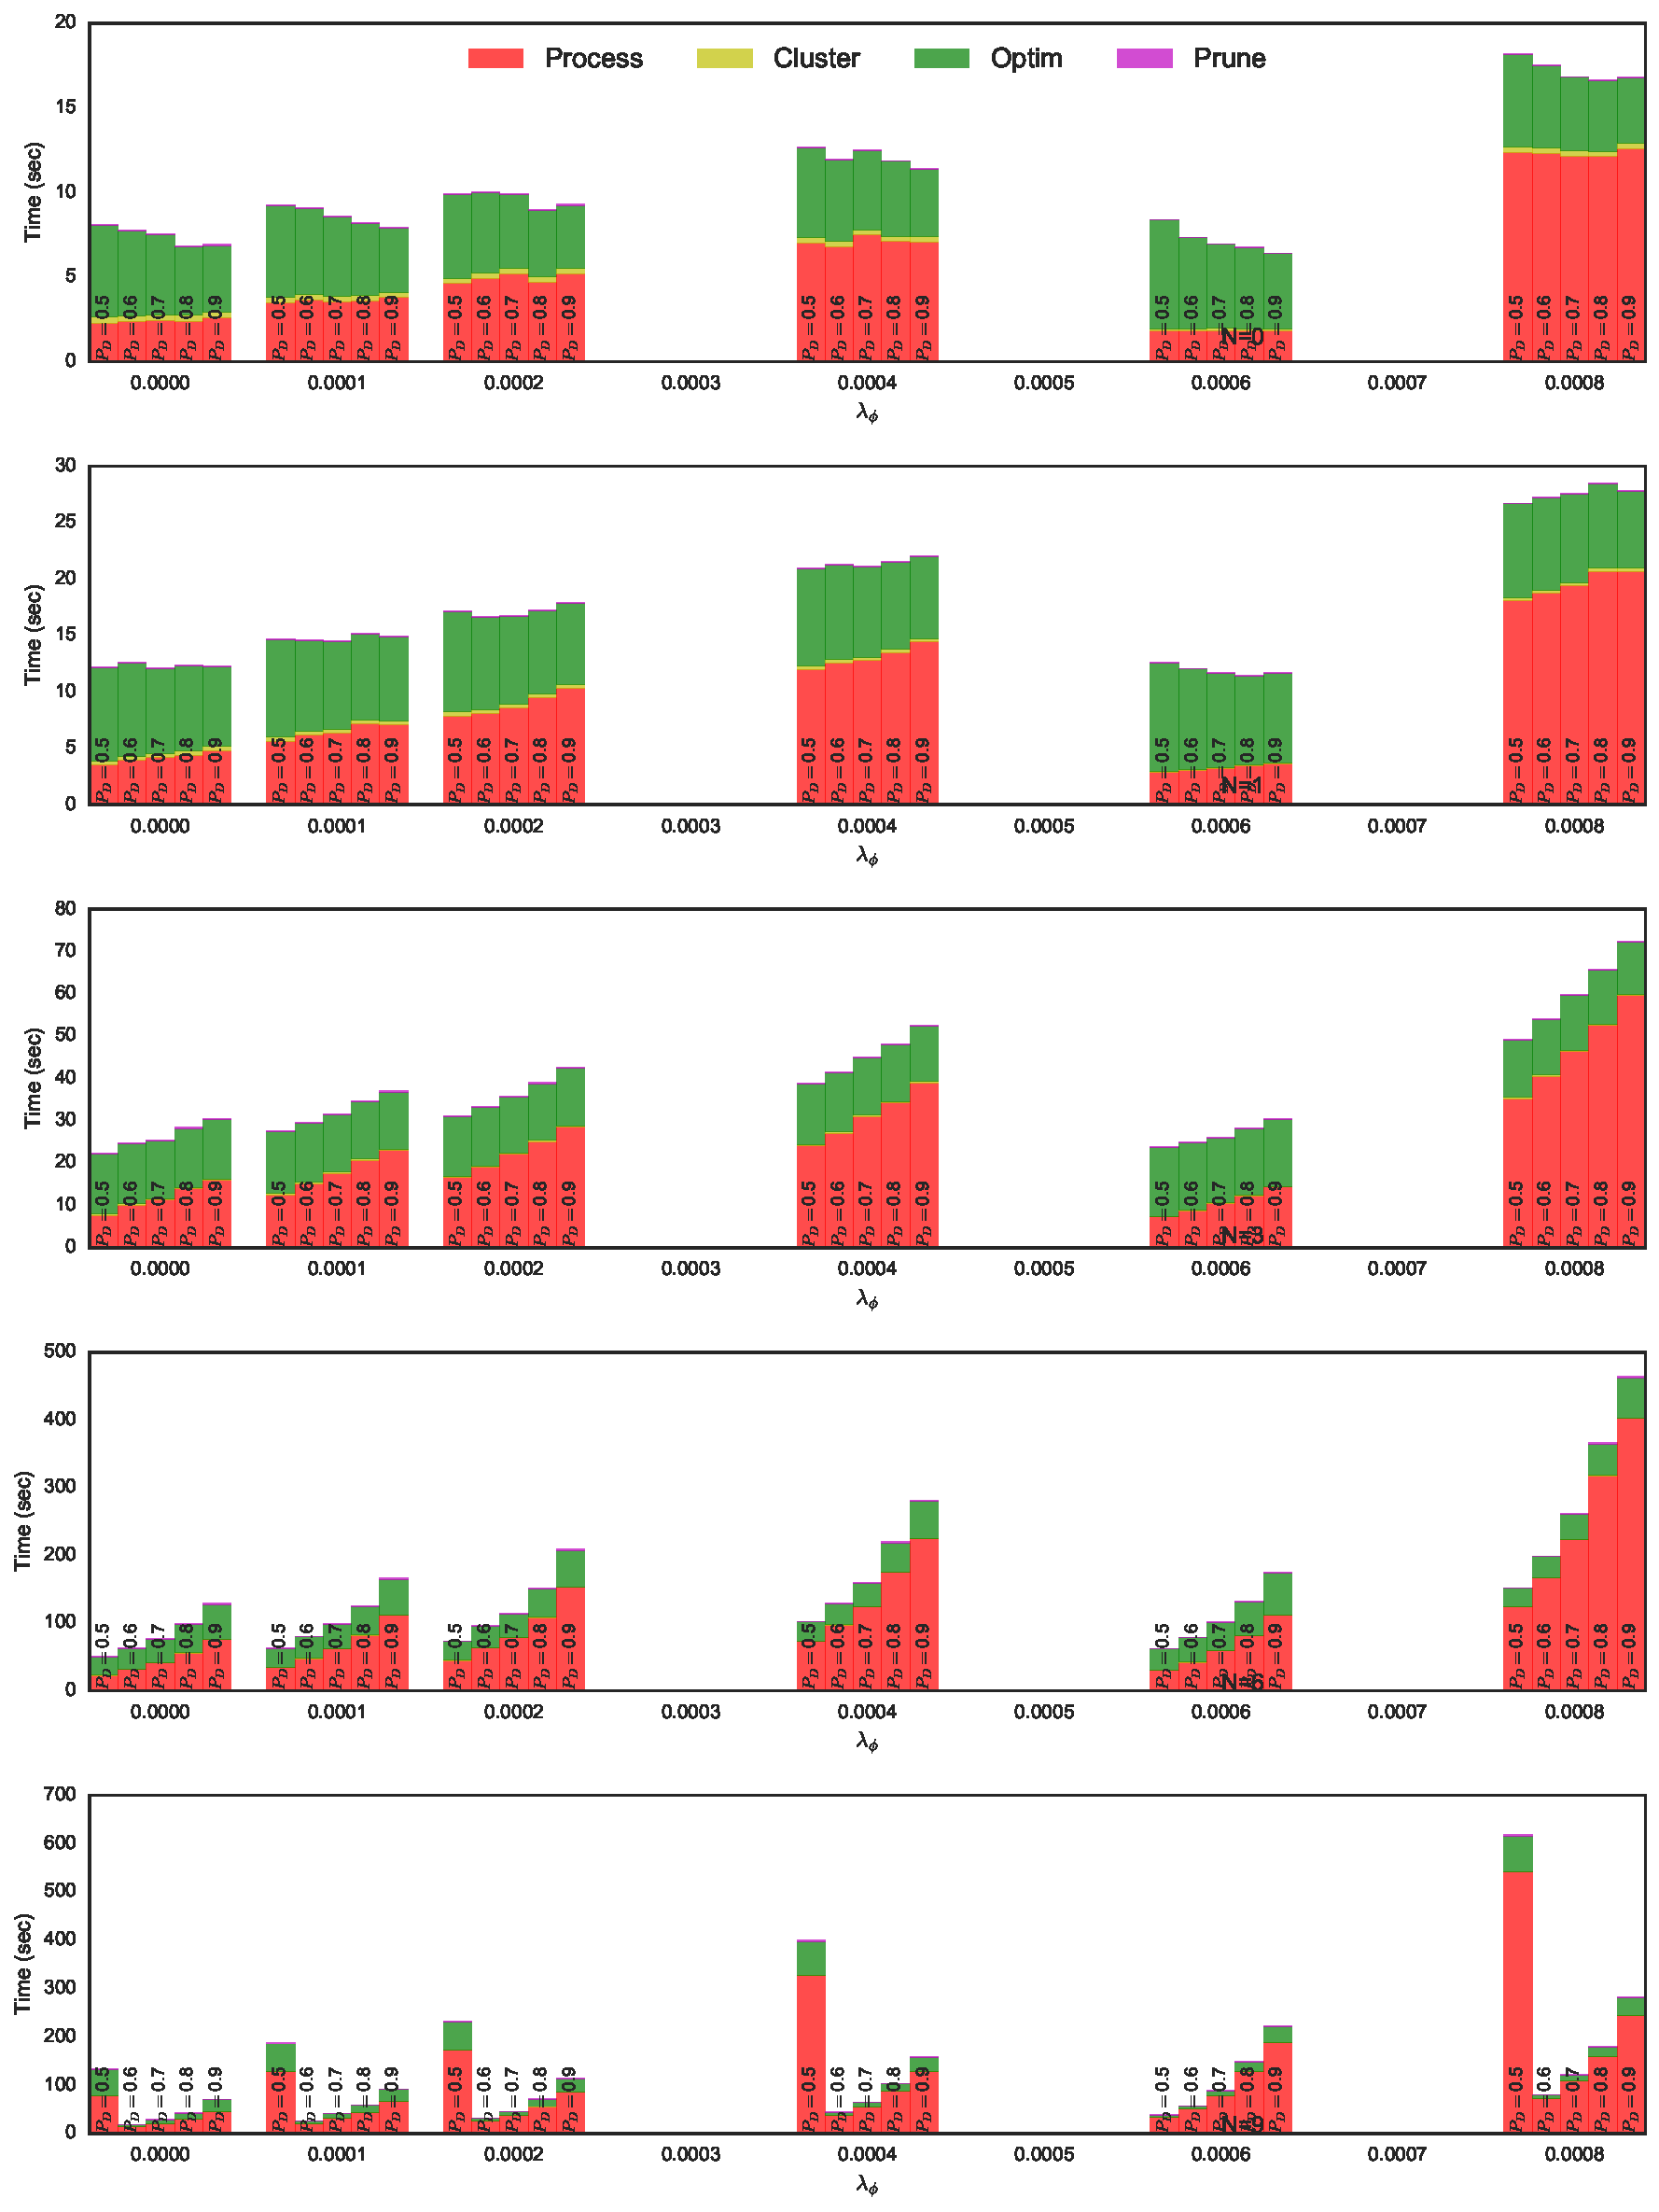
\includegraphics[width=\textwidth]{parallel_targets_1hz-CBC_runtimeLog}
	\caption{Scenario 5 - Run time log, CBC solver}
	\label{fig:runtimelog_scenario5-CBC}
\end{figure} 
\begin{figure}[H]
	\centering
	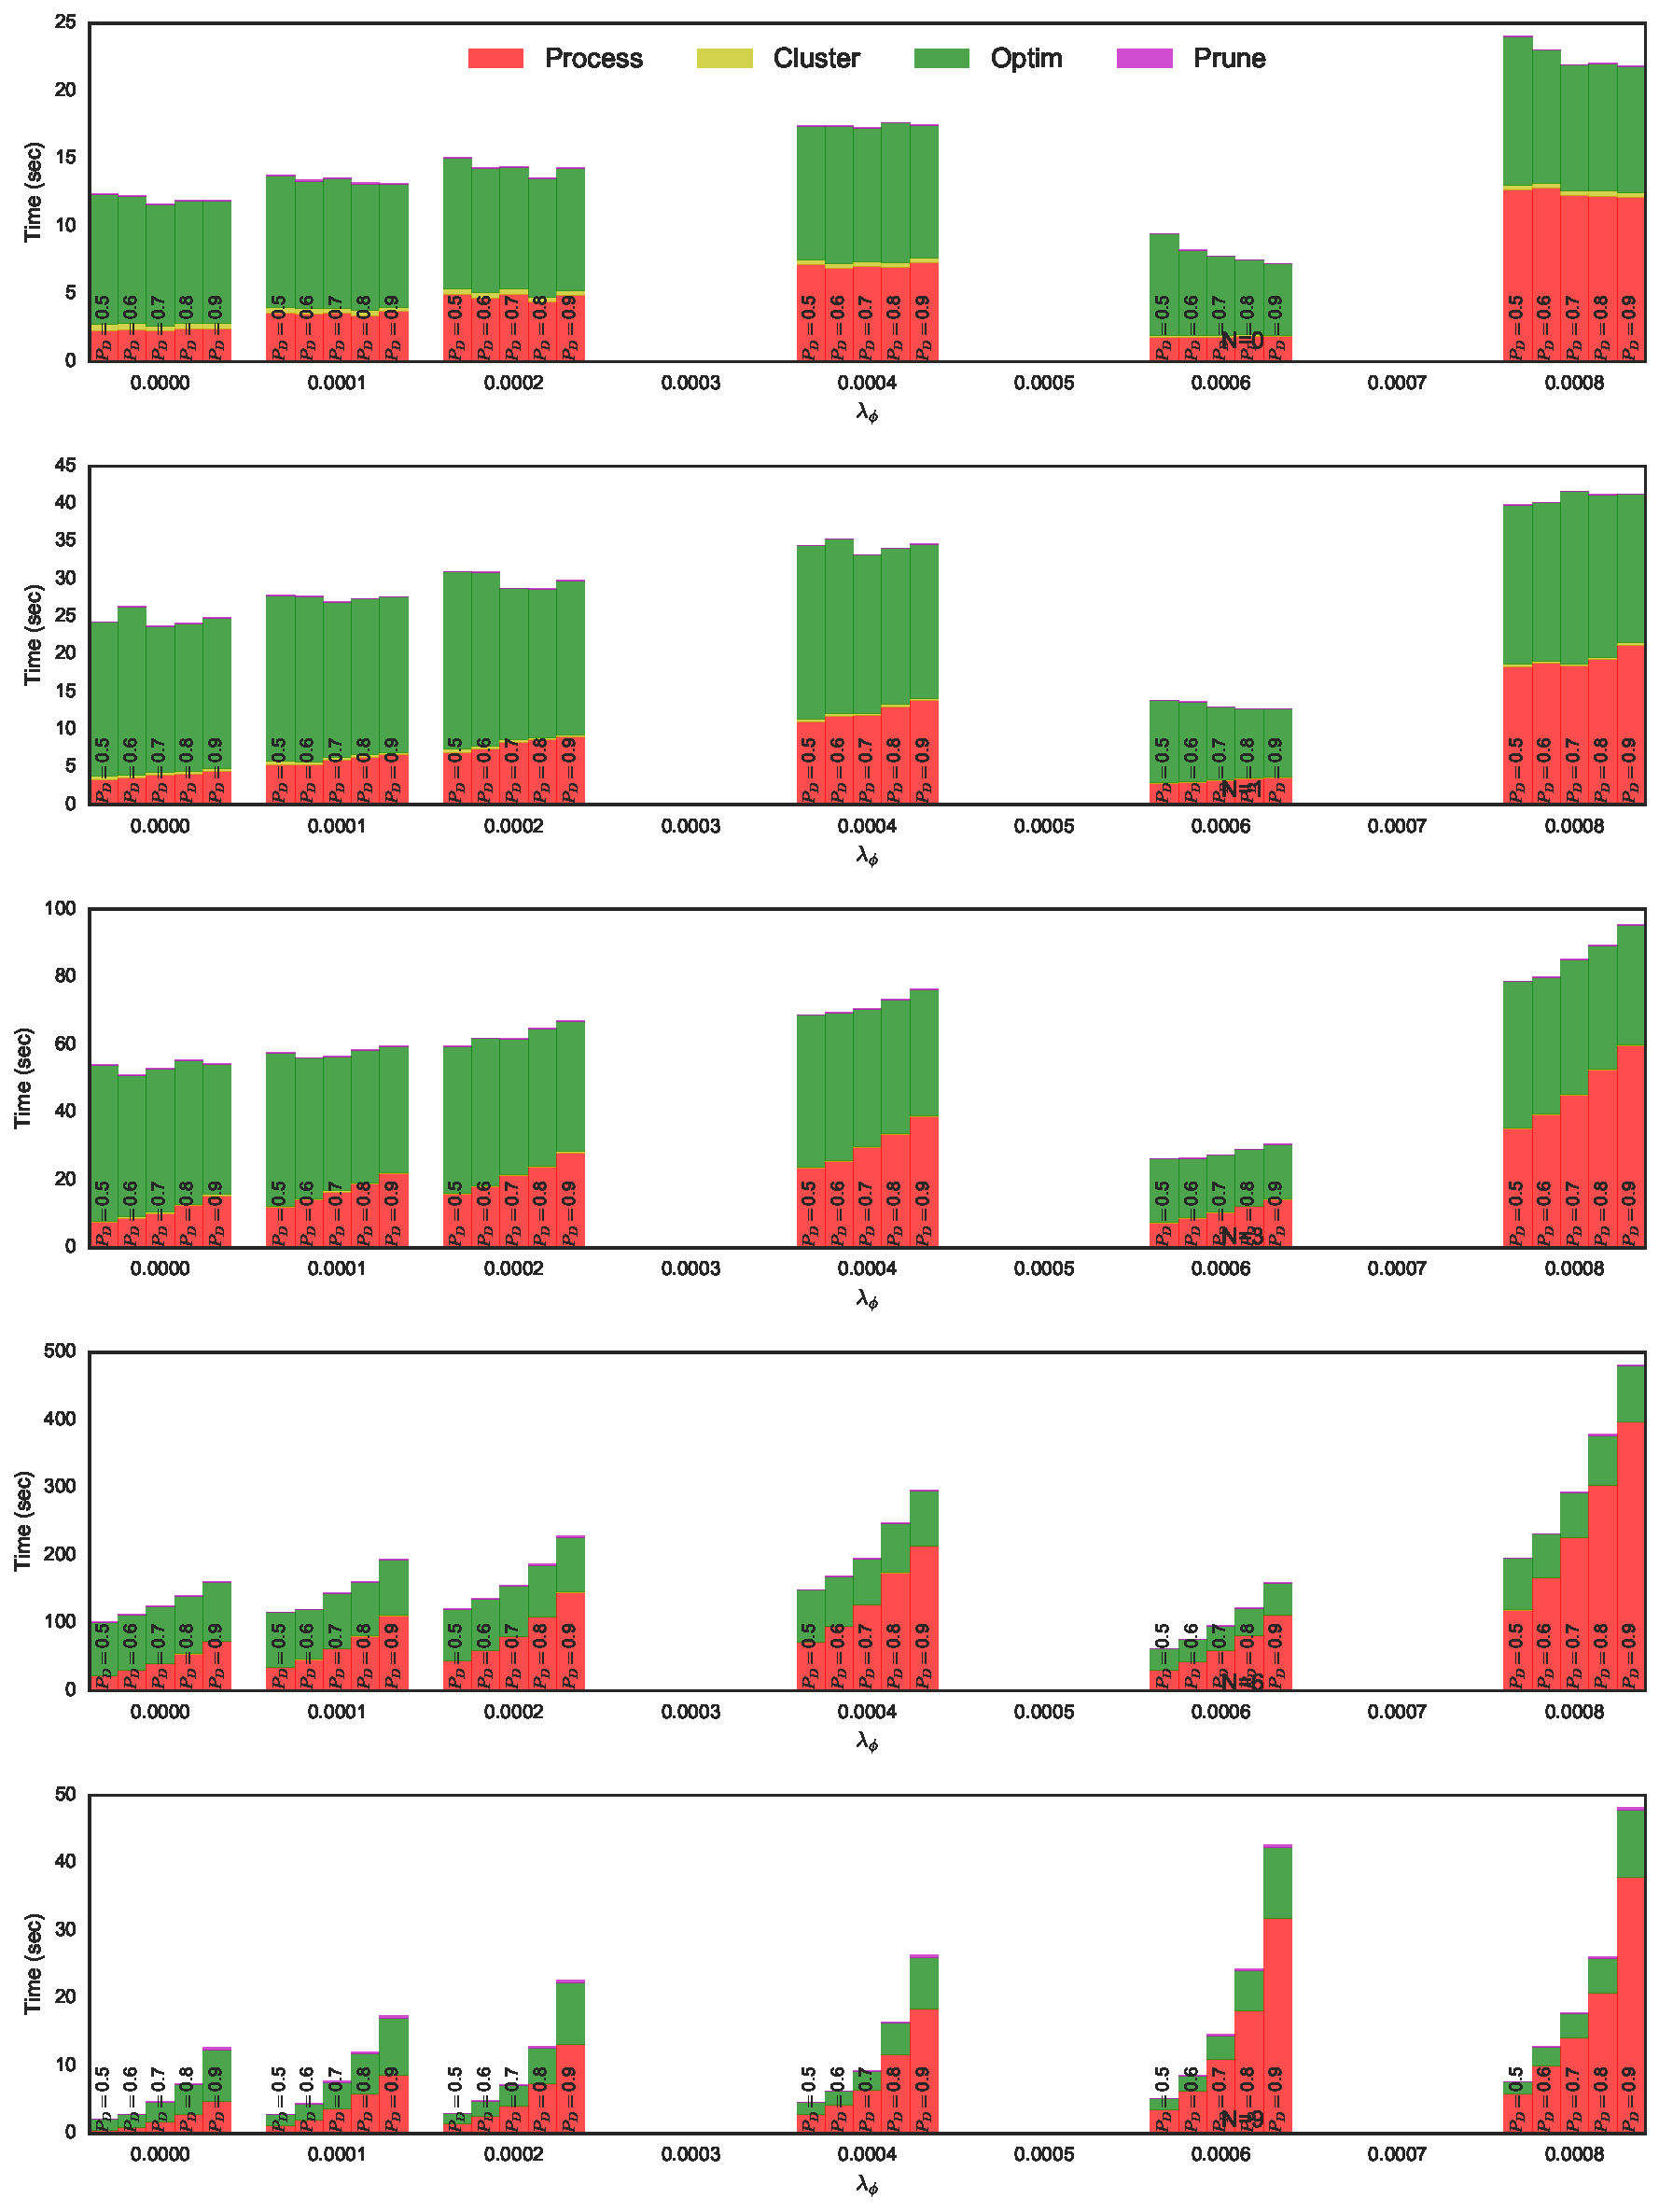
\includegraphics[width=\textwidth]{parallel_targets_1hz-CPLEX_runtimeLog}
	\caption{Scenario 5 - Run time log, CPLEX solver}
	\label{fig:runtimelog_scenario5-CPLEX}
\end{figure} 
\begin{figure}[H]
	\centering
	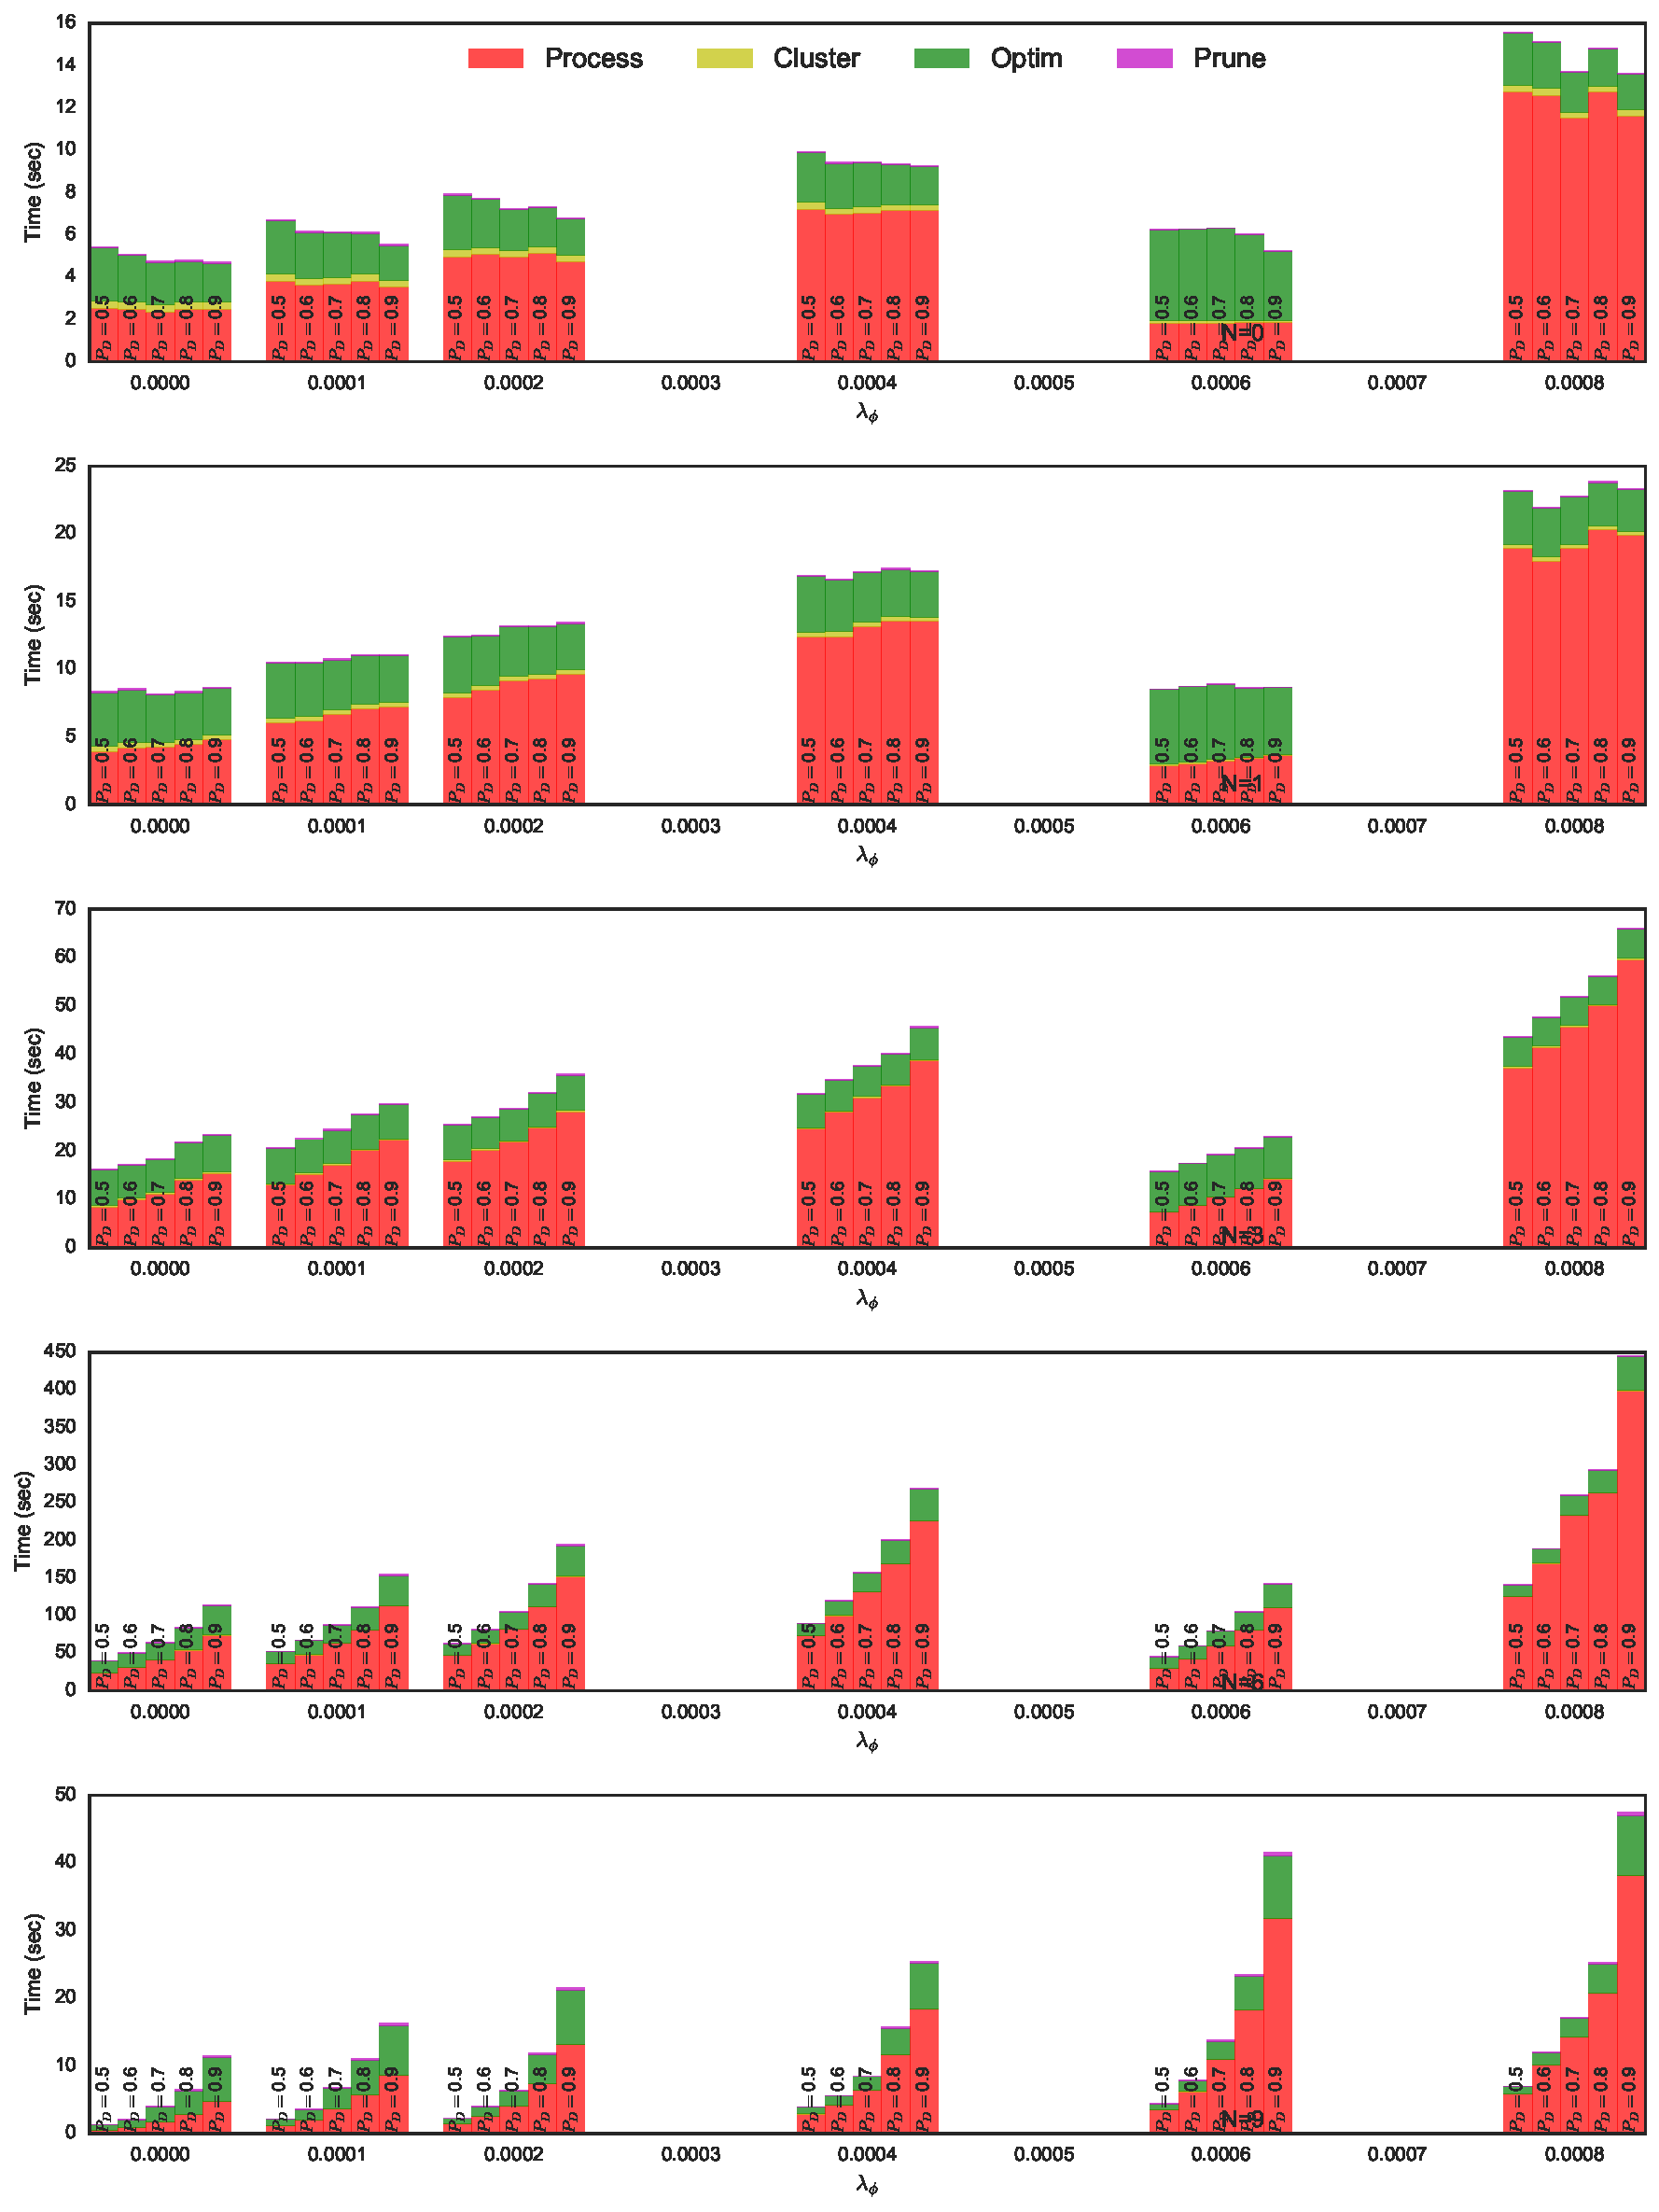
\includegraphics[width=\textwidth]{parallel_targets_1hz-GLPK_runtimeLog}
	\caption{Scenario 5 - Run time log, GLPK solver}
	\label{fig:runtimelog_scenario5-GLPK}
\end{figure} 
\begin{figure}[H]
	\centering
	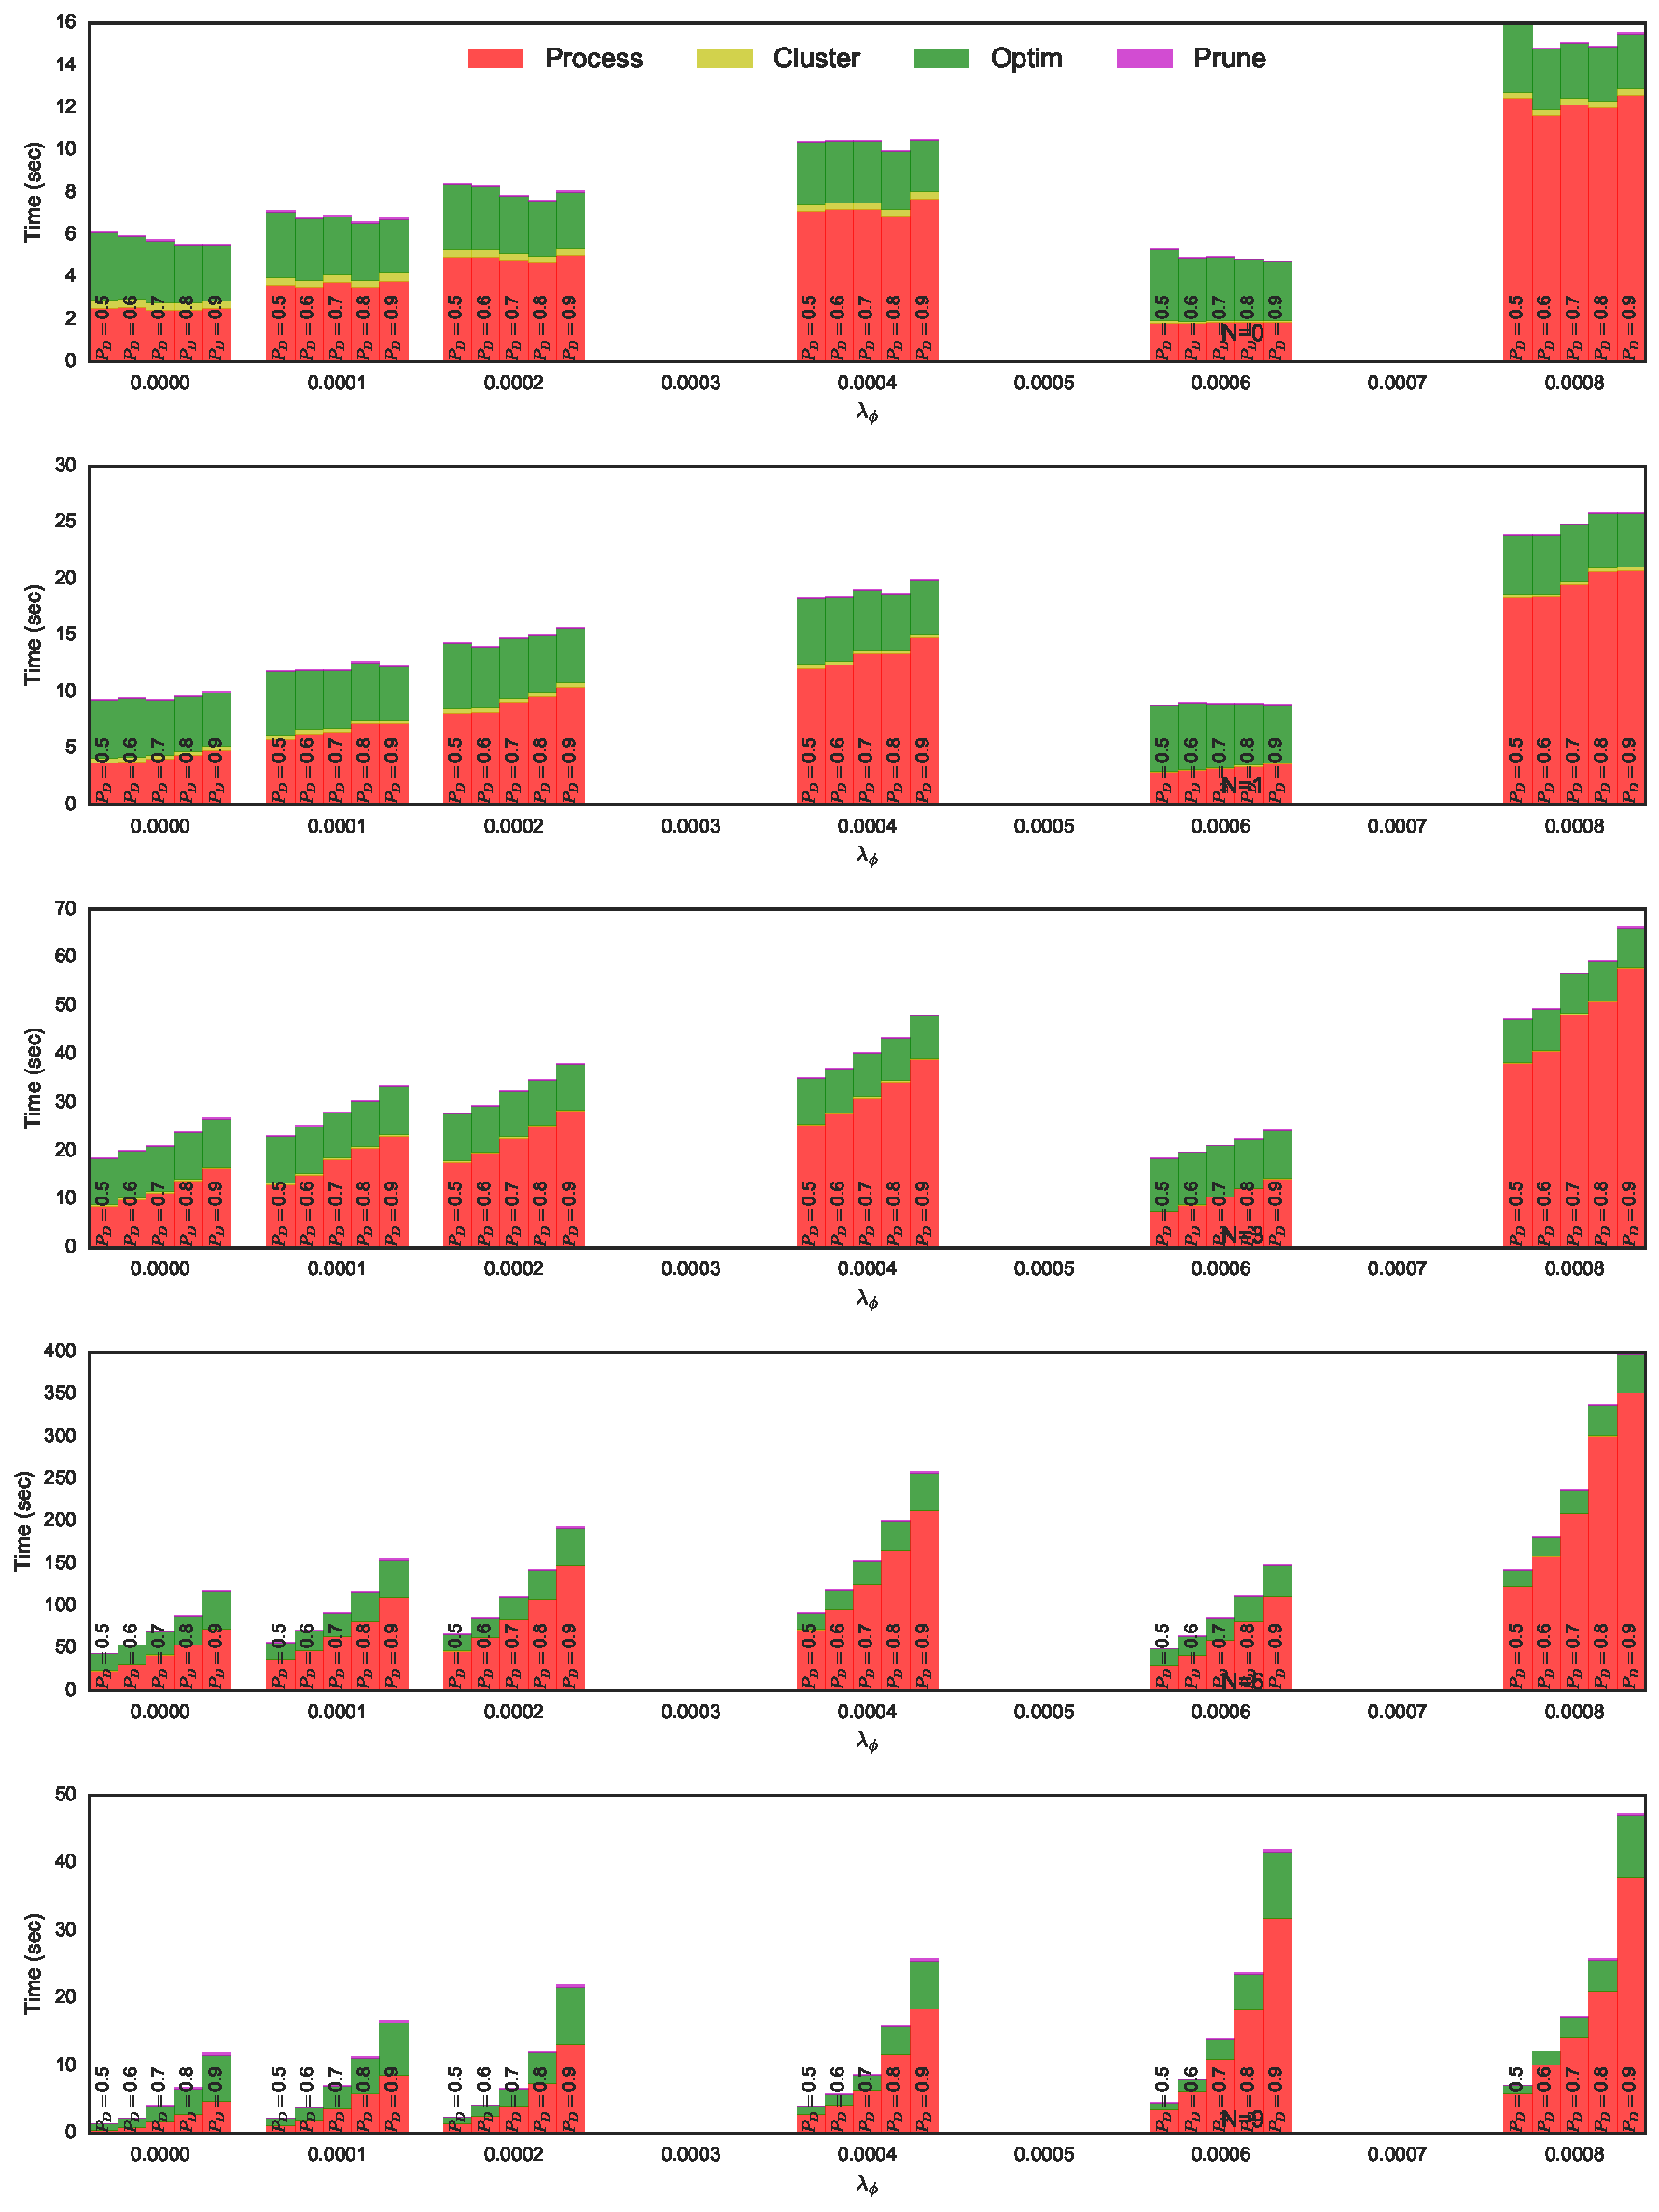
\includegraphics[width=\textwidth]{parallel_targets_1hz-GUROBI_runtimeLog}
	\caption{Scenario 5 - Run time log, GUROBI solver}
	\label{fig:runtimelog_scenario5-GUROBI}
\end{figure} 


\begin{figure}[H]
	\centering
	\includegraphics[width=\textwidth]{{parallel_targets_0.5hz-CBC_runtimeLog}.pdf}
	\caption{Scenario 6 - Run time log, CBC solver}
	\label{fig:runtimelog_scenario6-CBC}
\end{figure} 
\begin{figure}[H]
	\centering
	\includegraphics[width=\textwidth]{{parallel_targets_0.5hz-CPLEX_runtimeLog}.pdf}
	\caption{Scenario 6 - Run time log, CPLEX solver}
	\label{fig:runtimelog_scenario6-CPLEX}
\end{figure} 
\begin{figure}[H]
	\centering
	\includegraphics[width=\textwidth]{{parallel_targets_0.5hz-GLPK_runtimeLog}.pdf}
	\caption{Scenario 6 - Run time log, GLPK solver}
	\label{fig:runtimelog_scenario6-GLPK}
\end{figure} 
\begin{figure}[H]
	\centering
	\includegraphics[width=\textwidth]{{parallel_targets_0.5hz-GUROBI_runtimeLog}.pdf}
	\caption{Scenario 6 - Run time log, GUROBI solver}
	\label{fig:runtimelog_scenario6-GUROBI}
\end{figure}

%	\section*{tracker.py}
%	\inputminted[firstline=11,fontsize=\tiny, tabsize = 2, breaklines = true]{Python}{"../03Python/tomht/tracker.py"} 
	
%	\section*{helpFunctions.py}
%	\inputminted[firstline=2,fontsize=\tiny,tabsize = 2, breaklines = true]{Python}{"../03Python/tomht/helpFunctions/helpFunctions.py"}

%	\section*{kalmanFilter.py}
%	\inputminted[firstline=2,fontsize=\tiny,tabsize = 2, breaklines = true]{Python}{"../03Python/tomht/kalmanFilter/kalmanFilter.py"}

%	\section*{classDefinitions.py}
%	\inputminted[firstline=2,fontsize=\tiny,tabsize = 2, breaklines = true]{Python}{"../03Python/tomht/classDefinitions/classDefinitions.py"}

%	\section*{stateSpace.py}
%	\inputminted[firstline=2,fontsize=\tiny,tabsize = 2, breaklines = true]{Python}{"../03Python/tomht/stateSpace/pv/pv.py"}
\end{appendices}